\documentclass[12pt,preprint]{aastex}
\usepackage{url}
\usepackage{natbib}
\usepackage{graphicx}
\usepackage{subfig}
\usepackage{fixltx2e}
\usepackage{hyperref}
\usepackage{boxedminipage}
\usepackage{pdflscape}

%%%%%%%%%%%%%%%%%%%%%%%%%%%%%%%%%%%%%%%%%%%%%%%%%%%%
%%% author-defined commands
\newcommand\x         {\hbox{$\times$}}
\def\mic              {\hbox{$\mu{\rm m}$}}
\def\about            {\hbox{$\sim$}}
\def\Mo               {\hbox{$M_{\odot}$}}
\def\Lo               {\hbox{$L_{\odot}$}}
\newcommand{\water}   {H\textsubscript{2}O}
\newcommand{\ozone}    {O\textsubscript{3}}
\newcommand{\oxy}     {O\textsubscript{2}}

\captionsetup[figure]{labelformat=simple}
%%%%%%%%%%%%%%%%%%%%%%%%%%%%%%%%%%%%%%%%%%%%%%%%%%%%


\begin{document}

\title{Level 2 Photometric Calibration for the LSST Survey}

\author{
R. Lynne Jones\altaffilmark{1}, Tim Axelrod\altaffilmark{2},
{\v Z}eljko Ivezi{\'c}\altaffilmark{1},   David Burke\altaffilmark{3},
James G. Bartlett\altaffilmark{4}, \\
Gurvan Bazin\altaffilmark{4},
Guillaume Blanc\altaffilmark{4},
Alexandre Boucaud\altaffilmark{4},
Jean Marc Colley\altaffilmark{4},
Michel Cr{\'e}z{\'e}\altaffilmark{4}, \\ 
Mario Juric\altaffilmark{8},
C{\'e}cile Roucelle\altaffilmark{4}, 
Abhijit Saha\altaffilmark{5}, 
J. Allyn Smith\altaffilmark{7}, \\
Michael A. Strauss\altaffilmark{6},
Peter Yoachim \altaffilmark{1}\\
on behalf of 
The Photometric Calibration Team \\ 
Docushare-8123, 07/01/13 \\
}
\altaffiltext{1}{University of Washington}
\altaffiltext{2}{University of Arizona}
\altaffiltext{3}{SLAC National Accelerator Laboratory}
\altaffiltext{4}{APC, Universite Paris Diderot}
\altaffiltext{5}{NOAO}
\altaffiltext{6}{Princeton University}
\altaffiltext{7}{Austin Peay State University}
\altaffiltext{8}{LSST Corp}

% Gurvan Bazin
% 1- Department of Physics, Ludwig-Maximilians-Universit\"at, Scheinerstr. 1, 81679 Munich, Germany
%2- Excellence Cluster Universe, Boltzmannstr. 2, 85748 Garching, Germany
%3. APC - Universite Paris Diderot - Paris 7, Paris, France



\begin{abstract}
This document describes the photometric calibration procedure for LSST
Data Release catalogs. This procedure will use specialized hardware, 
an auxiliary telescope, an atmospheric water vapor measurement system, and narrow-band dome screen illuminator, to
measure the wavelength dependence of the atmospheric and hardware
response functions, together with a self-calibration procedure that
leverages multiple observations of the same sources over many epochs,
to deliver 1\%-level photometry across the observed sky.
\end{abstract}

\tableofcontents

\section{Introduction}

LSST is required to deliver photometry with 1\% uniformity and
0.5\% repeatability across the observed
sky and under a wide range of observing conditions. This represents at least a
factor of two improvement over current wide-field surveys such as
SDSS, CFHTLS, and PanSTARRS. This factor of two improvement will have a major impact on
science deliverables because it implies that the error volume in the
five-dimensional LSST color space will be over thirty times smaller
than for SDSS-like photometry. This smaller error volume will improve
source classification and the precision of quantities such as
photometric redshifts for galaxies and photometric metallicity for
stars.  For example, a given spectral energy distribution (SED)
corresponding to some galaxy type produces a line in the $ugrizy$
multi-dimensional color space when redshifted, where the position of
the galaxy along that line in $ugrizy$ space is a function of
redshift. Different galaxy SEDs produce lines that are often close to
each other in $ugrizy$ space and sometimes even cross. The smaller the
error volume around an observed galaxy's measured $ugrizy$ colors, the
smaller the number of different lines (thus, different SEDs) and
different positions along the line (thus, different redshifts) which
will be consistent with the measurement. The same conclusion is valid
in the case of algorithms that estimate stellar effective temperature
and metallicity, as well as any other model-based interpretation of
measurements. Furthermore, the smaller error volume per source is
advantageous even in the absence of any models. Two sources whose
color differences produce a value of $\chi^2$ per degree of freedom of
1, will have a $\chi^2$ per degree of freedom of 4 when the errors are
halved. In case of five degrees of freedom, $\chi^2$ pdf $>4$ will
happen by chance in only 0.1\% of all cases. Therefore, the ability to
reliably detect color differences between sources is a strong function
of photometric errors.

SDSS is widely credited with pioneering high accuracy photometry for large
surveys, and it is instructive to compare its photometric calibration procedure with LSST's.
The factor of two reduction in photometric error results from two major differences
between the surveys. First, each source will receive hundreds of
observations over the ten years of the LSST survey, a much greater number
than possible with SDSS. These series of
repeat observations will be used to self-calibrate the photometric
system across the sky and for each observation (akin, but not
identical to, the uber-calibration procedure used by SDSS
\citep{Padmanabhan2008}), allowing LSST to operate in a wide variety
of conditions. Secondly, the wavelength dependence of the hardware and
atmospheric transmission response functions will be measured with
auxiliary instrumentation on sufficiently fine angular and temporal
scales to enable their explicit inclusion in the calibration
procedure, rather than resorting to traditional approximations such as
linear color terms. SNLS re-processing of CFHT Legacy Survey data
found these color-dependent terms to be a significant contributor to
photometric calibration errors \citep{Regnault2009}, on
the level of several percent.

This document describes the calibration requirements and processes for
LSST Data Release photometry. At each Data Release, there will be a
complete recalibration of all data acquired to that point, on
approximately an annual schedule.  These data products are referred to
as Level 2 Data Products.  There will
also be a separate photometric calibration process that provides
near real-time, but lower quality, photometry for quality assurance,
generation of alerts, and other quantities required on a nightly
basis. This Level 1 photometric
calibration process is not discussed here.

Section~\ref{sec:photoreq} reviews the survey requirements for
photometric calibration, while Section~\ref{sec:calib_overview}
describes the foundation of LSST's calibration procedure, first
motivating this procedure by describing the transmission of flux
through the atmosphere and LSST system and then from the calibration
point of view, trying to recreate the flux from the ADUs measured
by the detector.
Sections~\ref{sec:photons2counts} and \ref{sec:counts2photons}
describe those aspects in some detail.
Section~\ref{sec:calib_external} describes how the LSST's internal
photometric scale is tied to external references.
Section~\ref{sec:calib_hardware} describes the hardware required
to realize the calibration process.
Section~\ref{sec:error_budget} presents the error budget for each step of the 
calibration procedure.
Section~\ref{sec:verification} describes how we will verify that the
calibration system functions as designed, and meets the science
requirements, first during the construction phase, and later during
survey operations.
Section~\ref{sec:software} describes the implementation of the calibration process
in software that will be part of LSST Data Management.
Finally, Section~\ref{sec:risks} discusses the risks that remain in
the implementation of the calibration process, and the steps we are 
taking to mitigate them.


\section{Photometric Requirements}
\label{sec:photoreq}

The LSST Science Requirements Document (SRD) provides a set of
requirements on the annual Data Release (Level 2) photometry.  These
requirements are extended in the XXX (OSS) to cover aspects which are
too detailed for the SRD.   based on
measurements of bright, unresolved, isolated, non-variable objects
from individual LSST visits. 
{\bf TODO - address what these requirements actually apply to. MS stars vs other SEDs and reference App C. Also be explicit that calibration is based on objects with well-known SEDs - i.e. MS stars. }
Bright implies that the
measurement of the star's brightness is not dominated by photon
statistics, approximately 1-4 magnitudes fainter than the saturation
limit in a given filter. Isolated implies that the star can be
successfully de-blended from background galaxies and other
stars. Non-variable objects are intrinsically not variable; these will
be identified in an iterative fashion from the many epochs of LSST
observations. The SRD specifications are: 
\begin{enumerate}
\item{{\bf Repeatability:} the median value of the photometric scatter
for each star (the rms of calibrated magnitude measurements around the
mean calibrated magnitude) shall not exceed 5 millimags in $gri$, 7.5
millimags in $uzy$ for bright, unresolved, isolated, non-variable
objects. No more than 10\% of these objects should have a photometric
scatter larger than 15 mmag in $gri$, 22.5 mmag in $uzy$.  This
specifies the distribution of photometric errors ($\sigma$) and
constrains both the repeatability of extracting counts from images and
the ability to monitor (or model) the changes in the system
response. It could be thought of as requiring the photometry
of a single source to be consistent over
time. \label{repeatability_req}}
\item{{\bf Uniformity:} the rms of the internal photometric zeropoint
error (for each visit) shall not exceed 10 millimags in $grizy$, 20 millimags in $uzy$,
where the zeropoint for each visit is determined using bright, unresolved, isolated, non-variable
sources. No more than 10\% of these sources should be more than 15
mmag in $gri$ or 22.5 mmag in $uzy$ from the mean internal zeropoint.
This places a constraint on the stability of the photometric system
across the sky as well as an upper limit on various systematic
errors, such as any correlation of photometric calibration with
varying stellar populations (or colors). This makes the photometry of
many sources comparable over the entire sky, and when combined with
the previous requirement, creates a stable photometric system across
the sky and over time, in a single filter. \label{uniformity_req}}
\item{{\bf Band-to-band photometric calibration:} The absolute
band-to-band zeropoint calibration for main sequence stars must be
known with an rms accuracy of 5 millimags for any color not involving $u$
band, 10 millimags for colors constructed with $u$ band
photometry. This places an upper limit on the systematic error in
the measurement of the system throughput as a function of
wavelength. This requirement ties photometric measurements in
different filters together, enabling precise measurement of colors. 
\label{color_req}}
\item{{\bf Absolute photometric calibration:} The LSST photometric
system must transform to an external physical scale ({\it e.g.} AB
mags) with an rms accuracy of 10 millimags. This requirement not only
ties LSST internal photometry to photometry obtained from other
telescopes, using other photometric systems, but also ties LSST
internal photometry to a real physical scale. This places a constraint
on the upper limit of the systematic error in the measurement of the
total system throughput. This final step enables LSST photometry to be
compared directly to data from other telescopes or to models ({\it
e.g.} such as determining the albedo of an asteroid with a known
diameter). \label{abs_req}}
\end{enumerate}

Requirements \ref{repeatability_req} and \ref{uniformity_req} must be
met by measuring and then correcting for changes in hardware and
atmospheric transmission as a function of time, location in the sky or
focal plane, and result in a relative calibration within a single
filter. Requirements \ref{color_req} and \ref{abs_req} require
comparison of LSST measurements to externally calibrated
spectrophotometric standards, providing a relative calibration from
filter to filter as well as an absolute physical scale for the overall
system.  Performance of the LSST system regarding requirement
\ref{repeatability_req} can be verified by simply measuring the rms of
the calibrated magnitude measurements. Verification of requirement
\ref{uniformity_req} is more complicated; in a simulated system it is
simple to compare the (simulated, thus known) true magnitudes of the
stars to the best-fit magnitudes produced after calibration. {\bf TODO forward reference new section on verification - Tim to write} 
In operations, this will be verified using a combination of simulations,
comparisons to known standards, and evaluation of science outputs such
as stellar locus diagrams. These last two tests are also relevant to
verifying the final two requirements, \ref{color_req} and
\ref{abs_req}.

{\bf TODO - Lynne (or someone) to verify consistency with new SRD reqs, *after* updating rest of doc and seeing effect of including new SEDs in SRD requirements. Plus need update of SRD to verify}. 


\section{The Photometric Calibration Process}
\label{sec:calib_overview}

In traditional photometric calibration, a set of standard stars are
observed at a range of airmasses to calculate zeropoint offsets and
(typically) a single color-dependent extinction curve per night. With care,
this approach can deliver 1\% photometry in stable photometric conditions.
Such programs typically follow only a few objects, and devote roughly equal
time to standards and program objects.   This approach fails for a survey like
LSST, for at least two reasons.  First, from a calibration point of view, 
the very wide field and multiple detector array mean that effectively a large number of instruments must be
calibrated rather than just one.
Second, historical weather data from Cerro Pach\'{o}n tells us
only 53\% of the available observing time can be considered
photometric even at the 1--2\% level. To take advantage of the full
85\% of the available observing time which is usable (total cloud
extinction less than 1.5 magnitudes), and to reach the SRD specified
requirements -- 0.5\% level photometric repeatability and 1\%
photometric uniformity -- requires a new approach.


This new approach, variants of which are already in use at PanSTARRS and DES,
{\it directly} measures the system throughput as a function of wavelength, 
focal plane position, and time.  Further, the {\it
normalization} of the throughput in each observation (the gray-scale
zeropoint) and the {\it shape} of the throughput curve (the color
dependent terms), are explicitly separated and measured with separate procedures
for both the telescope system response and the atmospheric transmission.  
This calibration system requires various
pieces of hardware to conduct these optimized measurements. We briefly
describe them here, with full descriptions in Section~\ref{sec:calib_hardware}:

\begin{itemize}
\item{A dome screen projector designed to provide uniform
    ($\sim10\%$ variation) illumination across the field of view, while
    minimizing stray light. This projector system will have the
    capability to not only illuminate the screen with broadband white
    light, but also narrow-band light to measure the system response
    at individual wavelengths. The narrow-band light will be generated
    by a tunable laser, capable of producing light from $300-1100$~nm
    and tunable in 1~nm increments. The brightness of the screen is measured 
    with a NIST-calibrated photodiode, so that the relative intensity at different 
    wavelengths is precisely determined. } 
\item{A 1.2-m auxiliary telescope with an $R \approx 400$ spectrograph,
    located adjacent to the LSST itself. This auxiliary telescope will
    obtain spectra of a chosen set of atmospheric probe stars across the sky to
    determine an atmospheric absorption model.} 
\item{Water vapor monitoring system, consisting of a GPS system and a 
    microwave radiometer attached copointed with the LSST telescope, and monitoring 
    the same field of view.  This supplements the auxiliary telescope spectra, which are
    unable to track the sometimes rapid variations of water vapor in time and space.}  
\end{itemize}

An overview of the entire calibration process, from science observation
to calibrated photometric measurements, together with the required
calibration data products is shown in
Figures \ref{fig:overview_flowchart1}, \ref{fig:overview_flowchart2}, 
\ref{fig:overview_flowchart3}, and \ref{fig:overview_flowchart4}.  
Note that four classes of objects participate in the calibration process in different ways:
\begin{itemize}
\item Standard stars.  These are stars whose absolute flux as a function of wavelength above the atmosphere is precisely known.  This class contains only a few members, perhaps as few as ten.  Their role is to enable the self calibration process to set absolute zeropoints for each band, and to allow testing of the SRD uniformity requirements.  See Section~\ref{sec:calib_external}.
\item Calibration stars.  These are stars that densely cover the sky, with typical spacings between stars of order 1 arcminute.  Unlike standard stars, neither their SEDs nor their absolute fluxes are precisely known, and their standard magnitudes are determined by the self calibration process.   They have been selected to be on the stellar main sequence, to be nonvariable, and to be relatively isolated so that their photometry is not degraded by crowding effects.
\item Atmospheric probe stars.   These are bright stars of known type, distributed roughly uniformly over the LSST sky, which yield high SNR spectra from the auxiliary telescope.  
\item Science objects.  Calibration of science objects utilizes the results of processing the standards and the calibration stars, and the measurement of the system bandpass.   If an SED is supplied for an object, an accurate standard magnitude can then be calculated.
\end{itemize}

The following section will provide a more in-depth overview of the
calibration process. We will start with a review of what
is physically happening to photons in their path toward the focal
plane, and then outline how LSST will translate the
measured ADU counts back to fluxes above the atmosphere.



\begin{boxedminipage}{6.5in}
We find it helpful to define four different magnitudes, and their associated fluxes:
\begin{itemize}
\item{$m_b^{inst}$, the instrumental magnitude.  $m_b^{inst} = -2.5 log10(C_b^{obs})$, where $C_b^{obs}$ are the instrumental counts (ADU) that are attributed to the object}
\item{$m_b^{nat}$, the natural magnitude.  This is the magnitude in the AB system that would be measured for the object if it were measured through the actual normalized system bandpass, $\phi_b^{obs}(\lambda)$, at the top of the atmosphere.  This bandpass varies
from exposure to exposure.  See equations \ref{eqn:Fb} and \ref{eqn:natmag}. $m_b^{nat} = m_b^{inst} + Z_b^{obs}$}
\item{$m_b^{std}$}, the standard magnitude.  This is the magnitude in the AB system that would be measured for the object if it were measured through the standard normalized system bandpass, $\phi_b^{std}(\lambda)$, at the top of the atmosphere.  This bandpass is 
selected as part of the survey design, and does not vary.  See equation \ref{eqn:stdFlux}. 
\item{$m_b^{corr}$, the SED corrected instrumental magnitude.  This is the standard magnitude, but with an unknown gray zeropoint correction, which will be removed by self calibration.  These magnitudes are the input to self calibration. $m_b^{corr} = m_b^{inst} + \Delta m_b^{obs}$}
\end{itemize}
These quantities are related through equations \ref{eqn:mag2counts} and \ref{eqn:mag2counts}.
\end{boxedminipage}

\section{From Flux to Counts}
\label{sec:photons2counts}

We first consider how the photons from an astronomical object make their
way to the detector and are converted into counts (ADUs), paying attention to the various
temporal or spatial scales for variability might arise in the LSST
system to affect the final ADU counts. 

Given $F_\nu(\lambda, t)$ --
the specific flux\footnote{Hereafter, the units for specific
flux (flux per unit  are Jansky (1 Jy = 10$^{-23}$ erg cm$^{-2}$ s$^{-1}$
Hz$^{-1}$). The choice of $F_\nu$ vs. $F_\lambda$ makes the flux
conversion to the AB magnitude scale more transparent, and the choice
of $\lambda$ as the running variable is more convenient than the
choice of $\nu$. Note also, while $F_\nu(\lambda,t)$ (and other
quantities that are functions of time) could vary more quickly than
the standard LSST exposure time of 15s, it is assumed that all such
quantities are averaged over that short exposure time, so that $t$
refers to quantities that can vary from exposure to exposure. }
(flux per unit frequency) of an astronomical object at
the top of the atmosphere -- at a position described by ($alt$,$az$),
the total flux from the object transmitted through the atmosphere to the telescope pupil is
\begin{equation}
\label{eqn:Fpupil}
   F_\nu^{pupil}(\lambda,alt,az,t) = F_\nu(\lambda, t) \, S^{atm}(\lambda,alt,az,t),
\end{equation}
where $S^{atm}(\lambda,alt,az)$ is the (dimensionless) probability that a photon of 
wavelength $\lambda$ makes it through the atmosphere,
\begin{equation}
\label{eqn:atmTau}
   S^{atm}(\lambda,alt,az,t)   = {\rm e}^{-\tau^{atm}(\lambda,alt,az,t)}.
\end{equation}
Here $\tau^{atm}(\lambda,alt,az)$ is the optical depth of the
atmospheric layer at wavelength $\lambda$ towards the position
($alt$,$az$). Observational data \citep{Stubbs2007b, Burke2010b} show
that the various atmospheric components which contribute to absorption
(water vapor, aerosol scattering, Rayleigh scattering and molecular
absorption) can lead to variations in $S^{atm}(\lambda,t)$ on the
order of 10\% per hour. Clouds represent an additional gray (non-wavelength
dependent) contribution to $\tau^{atm}$ that can vary even more
rapidly, on the order of 2--10\% of the total extinction at $1^{\circ}$
scales within minutes \citep{Ivezic2007}.

Given the above $F_\nu^{pupil}(\lambda,alt,az,t)$, the total ADU
counts transmitted from the object to a footprint within the field of
view at ($x$, $y$) can be written as
\begin{equation}
\label{eqn:Fpupil2counts}
    C_b(alt, az, x,y,t) = C \, \int_0^\infty {F_\nu^{pupil}(\lambda,alt,az,t) \, S_b^{sys}(\lambda,x,y,t) \lambda^{-1}d\lambda}.
\end{equation}
Here, $S_b^{sys}(\lambda,x,y,t)$ is the (dimensionless) probability
that a photon will pass through the telescope's optical path to be
converted into an ADU count, and 
includes the mirror reflectivity, lens transmission, filter
transmision, and detector sensitivity. The term
$\lambda^{-1}$ comes from the conversion of energy per unit frequency
into the number of photons per unit wavelength and $b$ refers to a particular filter, $ugrizy$. The
dimensional conversion constant $C$ is
\begin{equation}
\label{eqn:Cconstant}
        C = {\pi D^2 \Delta t \over 4 g h }  
\end{equation}
where $D$ is the effective primary mirror diameter, $\Delta t$ is the
exposure time, $g$ is the gain of the readout electronics (number of
photoelectrons per ADU count, a number greater than one), and $h$ is
the Planck constant. The wavelength-dependent variations in
$S_b^{sys}$ generally change quite slowly in time; over periods of
months, the mirror reflectance and filter transmission will degrade as
their coatings age. A more rapidly time-varying wavelength-dependent
change in detector sensitivity (particularly at very red wavelengths
in the $y$ band) results from temperature changes in the detector, but
only on scales equivalent to a CCD or larger.  There will also be
wavelength-dependent spatial variations in $S_b^{sys}$ due to
irregularities in the filter material; these are required by the
camera specifications to vary (at a maximum)
slowly from the center of the field of view to the outer edges,
equivalent to a bandpass shift on the order of 1-2\% of the effective
wavelength of the filter. Wavelength-independent (gray-scale)
variations in $S_b^{sys}$ can occur more rapidly, on timescales of a
day for variations caused by dust particles on the filter or dewar
window, and on spatial scales ranging from the amplifier level,
arising from gain changes between amplifiers, down to the pixel level,
in the case of pixel-to-pixel detector sensitivity variations.

From equation~\ref{eqn:Fpupil2counts} and the paragraphs above, we can
see that the generation of counts $C_b(alt,az,x,y,t)$ from photons is
imprinted with many different effects, each with different variability
scales over time, space, and wavelength. In particular the
wavelength-dependent variability (bandpass shape) is
typically much slower in time and space than the gray-scale variations
(bandpass normalization). These different scales of variability
motivate us to separate the measurement of the normalization of
$S_b^{sys}$ and $S^{atm}$ from the measurement of the
wavelength-dependent shape of the bandpass.

\subsection{Normalized bandpass response, $\phi_b(\lambda)$}
\label{sec:phi}

This then leads us to introduce a `normalized bandpass response
function', $\phi_b^{obs}(\lambda,t)$, that represents the true
bandpass response shape for each observation,
\begin{equation}
\label{eqn:PhiDef}
   \phi_b^{obs}(\lambda,t) =  {
     {S^{atm}(\lambda,alt,az,t)\, S_b^{sys}(\lambda,x,y,t) \,
       \lambda^{-1}} \over
     \int_0^\infty { {S^{atm}(\lambda,alt,az,t) \,
         S_b^{sys}(\lambda,x,y,t) \, \lambda^{-1}} \,d\lambda}}.
\end{equation}
Note that $\phi_b$ only represents {\it shape} information about the
bandpass, as by definition
\begin{equation}
\int_0^\infty {\phi_b(\lambda)  d\lambda}=1. 
\end{equation}
Using $\phi_b^{obs}(\lambda, t)$ we can represent the (true, total)
in-band flux of an object for each observation as
\begin{equation}
\label{eqn:Fb}
F_b^{obs}(t) = \int_0^\infty {F_\nu(\lambda,t) \,\phi_b^{obs}(\lambda,t) \, d\lambda},
\end{equation}
where the normalization of $F_b(t)$ corresponds to the top of the
atmosphere. Unless $F_\nu(\lambda,t)$ is a flat ($F_\nu(\lambda)=$
constant) SED, $F_b^{obs}$ will vary with changes in
$\phi_b^{obs}(\lambda,t)$ due simply to changes in the bandpass shape,
such as changes with position in the focal plane or differing
atmospheric absorption characteristics, {\it even if the source is
non-variable}.

To provide a reported $F_b^{std}(t)$ which is constant for
non-variable sources, we also introduce the `standardized bandpass response
function', $\phi_b^{std}(\lambda)$, a curve that will be defined before
the start of LSST operations (most likely during
commissioning). $\phi_b^{std}(\lambda)$ represents a typical hardware
and atmospheric transmission curve, minimizing the difference between
$\phi_b^{obs}(\lambda,t)$ and the standardized reported bandpass.
Now, 
\begin{equation}
\label{eqn:stdFlux}
F_b^{std}(t) = \int_0^{\infty} {F_\nu(\lambda,t) \,
  \phi_b^{std}(\lambda) \, d\lambda}, 
\end{equation}
is a constant value for non-variable sources. 

Magnitudes provide an easy way to conceptualize the relationship
between $F_b^{obs}$ and $F_b^{std}$, provided that we define a
`natural magnitude' 
\begin{equation}
\label{eqn:natmag}
m_b^{nat}  = -2.5\, log_{10} \left( {F_b^{obs} \over F_{AB}}  \right)
\end{equation}
where $F_{AB}$ = 3631 Jy. The natural magnitude, like $F_b^{obs}$ will
vary from observation to observation as $\phi_b^{obs}(\lambda,t)$
changes, even if the source itself is non-variable. The natural
magnitude can be translated to a `standard magnitude', $m_b^{std}$, as
follows:
\begin{eqnarray}
m_b^{nat} & = &-2.5\, log_{10} \left( {F_b^{obs} \over F_{AB}} \right) \\
& = & -2.5 \, log_{10} \left( { \int_0^\infty {F_\nu(\lambda,t) \,
    \phi_b^{obs}(\lambda,t) \, d\lambda} \over F_{AB} }  \right) \\
& = & -2.5 \, log_{10} \, \left( \left( { \int_0^\infty {F_\nu(\lambda,t) \,
    \phi_b^{obs}(\lambda,t) \, d\lambda} \over \int_0^\infty {F_\nu(\lambda,t) \,
    \phi_b^{std}(\lambda,t) \, d\lambda}} \right) \, \left( {\int_0^\infty {F_\nu(\lambda,t) \,
    \phi_b^{std}(\lambda,t) \, d\lambda} \over F_{AB}} \right) \right) \\
m_b^{nat} & = & \Delta m_b^{obs} + m_b^{std} \\
\label{eqn:Delta_m}
\Delta m_b^{obs} & = & -2.5 \, log_{10} \,  \left( { \int_0^\infty {F_\nu(\lambda,t) \,
    \phi_b^{obs}(\lambda,t) \, d\lambda} \over \int_0^\infty {F_\nu(\lambda,t) \,
    \phi_b^{std}(\lambda,t) \, d\lambda}} \right)
\end{eqnarray}
where $\Delta m_b^{obs}$ varies with the {\it shape} of the source
spectrum, $f_\nu(\lambda,t)$ and the {\it shape} of the bandpass
$\phi_b^{obs}(\lambda,t)$ in each observation. Note that $\Delta
m_b^{obs}=0$ for flat (constant) SEDs, as the integral of
$\phi_b(\lambda)$ is always one.  For non-variable sources,
$m_b^{std}$ will be non-variable as it represents the throughput in a
standardized bandpass, $\phi_b^{std}(\lambda)$.

The natural and standard magnitudes can be tied back to the counts
produced by the system by adding the correct zeropoint offsets. As
$\Delta m_b^{obs}$ removes all wavelength dependent variations in $m_b^{std}$,
\begin{eqnarray}
\label{eqn:mag2counts}
m_b^{std} & = & m_b^{inst} \, - \Delta m_b^{obs} + Z_b^{obs} \\
 & \equiv & m_b^{corr} + Z_b^{obs}
\end{eqnarray}
where
\begin{equation}
m_b^{inst} = -2.5\,log_{10}(C_b^{obs})
\end{equation}

The zeropoint correction here, $Z_b^{obs}$, contains only gray-scale
{\it normalization} effects, such as variations due to the flat field
or cloud extinction.  The SED corrected magnitude, $m_b^{corr}$, is the input to the Self Calibration block in 
Figure \ref{fig:overview_flowchart1}.



\subsection{Perturbations to the System Bandpass}
The normalized system bandpass will vary from exposure to exposure due to a myriad of effects.  The major ones are:
\begin{itemize}
\item{Atmospheric transmission variations.  The major wavelength-dependent sources of atmospheric absorption, Rayleigh scattering from molecules, molecular oxygen lines, ozone, water vapor, and aerosols, all vary in time and space, with widely varying temporal and spatial scales.  Even in the absence of intrinsic variation in the atmosphere, of course, the bandpass varies due to changing airmass.  This latter effect is compensated for in traditional photometric calibration, but the others are generally ignored}
\item{Long term variations in the throughput of the optical path due to contamination}
\item{Changing detector quantum efficiency, particularly in the y-band, due to varying focal plane temperature}
\item{Shifts in filter position with respect to the system optical axis, due to positioning jitter and gravity sag}
\end{itemize}

It bears repeating that every perturbation in general affects both the zeropoint, through the gray component of the perturbation, and the shape of the system bandpass, through the wavelength-dependent component.  The gray component is removed by the self calibration process, while the wavelength-dependent component must be separately characterized and removed (see Figure \ref{fig:overview_flowchart1}).  We are concerned here only about the latter effect, and discuss it for each of the above categories.

\subsection{Effects of Airmass Variation}

The effects of airmass variation on photometry is well known to all photometrists.   In fact, it is the only effect which is
always accounted for in photometric calibration, and quite often the only effect.   Figure \ref{fig:dmag_airmass} shows the effects
of variation over the full airmass range expected for the LSST survey.  There is a more subtle effect, however, which is important
because of the LSST's large field of view: the airmass can vary significantly from one side of the field to the other. For example,
if the field center is airmass 2.1, the airmass varies from 1.98 to 2.22 across the field.  Figure \ref{fig:dmag_fov} shows the error
that would be made in ignoring this effect.  This requires us to maintain an atmospheric model which can be interpolated
to any position in the focal plane.

\subsection{Effects of Atmospheric Variations}

The main components of wavelength-dependent atmospheric extinction are Rayleigh scattering from molecules; oxygen molecular lines; water vapor; ozone; and aerosols.   Rayleigh scattering and molecular oxygen extinctions are directly proportional to barometric pressure at the surface.  As is well known from looking at surface pressure charts, away from weather fronts the pressure varies significantly on timescales of hours or more and spatial scales of hundreds of km.  Variations can be much more rapid in the vicinity of fronts.   In any case, this component can be compensated for very accurately just by measuring the barometric pressure, and we do not further consider it here.  The other components are not so easily measured, and in the case of water vapor and aerosols, can display complex patterns of variability.  

Figures \ref{fig:CTIO_PWV}, \ref{fig:GeminiPWV}, and \ref{fig:PWV_satellite} give three different perspectives on historical water vapor variability in the vicinity of CP.  There are broad patterns in space (the E-W gradient), and in time (the regular seasonal variations).  There are large variabilities on top of these, amounting to several mm of PWV, which can occur in hours or less.   The biggest effect of water vapor is in the y-band, since it contains a strong water band (Figure \ref{fig:xx}).   Figure \ref{fig:KuruczPWV} shows the change in natural magnitude when the PWV is varied from 1mm to 6mm for a set of Kurucz stars.  The 4mm variation in PWV shown in Figure \ref{fig:GeminiPWV} would lead to a roughly +/-3mmag color-dependent scatter in calibration of y photometry, if not compensated for. 

While we do not have aerosol variability data for Cerro Pachon (CP), data from CASLEO, a site at 2550m in Argentina (\citep{CASLEO}) serves as a reasonable proxy.  Figure \ref{fig:CASLEO} shows the time history of aerosol optical depth at 675nm over a period of roughly a year.  The spiky nature of the data is notable, suggesting rapid variations on timescales of perhaps a few hours.  Figure \ref{fig:AerosolVar}, which shows a time-altitude profile of aerosol variations at a site in the US, backs up this impression.  Although the site is at much lower altitude than CP, there are nonetheless significant variation of aerosol extinction at altitudes above 3000m on time scales well under an hour, and we should expect similar variations at CP.  Determining the effects of aerosol variations on the system bandpass is more complex than for other atmospheric components, because the spectral shape of the aerosol extinction varies as well as its magnitude.  Figure \ref{fig:KuruczAerosol} shows the change in natural magnitude when the aerosol optical depth is varied from 0.04 mag to 0.16 mag, roughly the range of the CASLEO data, while keeping a constant spectral index of $\alpha = -1.7$.  Unlike water vapor, which affected the reddest bands most strongly, aerosols affect the bluest bands the most.  The effects in the u-band range from -5 mmag to +35 mmag, strongly dependent on star color.

Ozone is dominantly a stratospheric component of the atmosphere, and is routinely monitored by satellite.   There is little evidence for variations on short time or space scales, with most variation on a seasonal scale.   Figure \ref{fig:O3atCP} shows the overall variability of ozone at CP over a roughly 8 year period.  Figure \ref{fig:KuruczO3} shows the changes in the natural magnitudes for a variation in ozone by 50 Dobson units.   The effect is very small, except in the u-band, where it has a noticeable effect on red stars.

To summarize the effects of wavelength-dependent atmospheric variations, they are sufficiently large, and occur sufficiently rapidly, that they must be corrected by an atmospheric model with fidelity substantially greater than the traditional photometrist's extinction model.   The combination of the auxiliary telescope and the water vapor monitoring system will supply the data required for construction of these atmospheric models.  It is also worth emphasizing that correcting for these effects requires not only an accurate bandpass model, but also SEDs for the objects being calibrated.   Calibration stars will be picked from well defined stellar populations to minimize SED uncertainty.   SED determination for arbitrary science objects, such as supernovae and galaxies, will be more challenging, and may limit the accuracy of their photometric calibration.







\subsection{Throughput Variations Due to Contamination}

\subsection{Variations in Detector Quantum Efficiency}

\subsection{Throughput Variations Due to Filter Position Shifts}

\subsection{Putting it All Together}
Examples of the $\Delta m_b^{obs}$ due to variations in the shape of
the hardware and atmospheric response curves are shown in
Figure~\ref{fig:delta_mags} and Table~\ref{tab:delta_mags}. Two main
sequence stellar models \citep{Kurucz1993} -- one with temperature
35000K (blue) and one 6000K (red) -- were combined with three
different atmospheric response curves (with airmass X=1.0 with minimal
\water\, vapor, X=1.2 with a nominal amount of \water\,(the
`standard'), and X=1.8 with a large \water\,vapor content) and two
different hardware response curves (one `standard' and one shifted in
wavelength by 1\%) to illustrate the resulting changes in observed
natural magnitudes. In Figure~\ref{fig:delta_mags2}, the $X=1.8$
atmospheric response is combined with a $1\%$ shift (the maximum
allowed in the filter manufacturing specification from center to edge)
in filter bandpass, thus altering the hardware response, for many main
sequence Kurucz models spanning a range of $g-i$ colors; the resulting
changes in natural magnitudes are plotted.  These examples demonstrate
that the scatter in natural magnitudes induced by expected atmospheric
and hardware transmission curve shape changes alone (without any
gray-scale changes) can be much larger than the SRD repeatability
requirements would permit. Roughly speaking, these effects reach a level of about 
50 mmag.  This suggests that our measurement-based model of wavelength-dependent
effects must be accurate at the 90-95\% level.  This issue is discussed in detail in Section
\ref{sec:error_budget}



\begin{center}
\begin{table}[htb]
\caption{{\bf $\Delta m_b^{obs}$ due to variations in system and atmospheric
 bandpass shape (see also Fig~\ref{fig:delta_mags}). The first two
rows show the baseline (`standard') magnitude of the star. All other rows show the 
{\it change} in magnitude (in mmag) due to the variations listed at
left. Any value larger than 5~mmag would be larger than the RMS
scatter allowed by the SRD. {\it TODO color-code values larger than 5 mmag}} }
\begin{tabular}{l l | c c c c c c}
Bandpass & star &  $u$ (mag) & $g$ & $r$ & $i$ & $z$ & $y$ \\ \hline
Std (X=1.2) atm, std sys  &  red & 21.472 & 20.378 & 20.000 & 19.911 & 19.913 & 19.913 \\
Std (X=1.2) atm, std sys  &  blue & 19.102 & 19.503 & 20.000 & 20.378 & 20.672 & 20.886 \\ \hline \hline
 & & $\Delta u$ (mmag) & $\Delta g$  & $\Delta r$  & $\Delta i$ & $\Delta z$  & $\Delta y$ \\ \hline
Std (X=1.2), +1\% sys shift & red  & -31 & -22 & -8 & -2 & 1 & 1 \\
Std (X=1.2), +1\% sys shift & blue  & 9 & 17 & 20 & 20 & 16 & 16 \\ \hline
X=1.0, std sys & red  & 7 & 2 & 0 & 0 & -0 & -1 \\
X=1.0, std sys & blue  & -3 & -1 & -1 & -0 & 1 & -4 \\ \hline
X=1.0, +1\% sys shift & red & -24 & -20 & -8 & -1 & 1 & 0 \\
X=1.0, +1\% sys shift & blue & 7 & 16 & 19 & 20 & 18 & 12 \\ \hline
X=1.8, std sys  & red & -21 & -10 & -2 & -0 & 0 & 1 \\
X=1.8, std sys  & blue & 8 & 8 & 4 & 2 & -1 & 6 \\ \hline
X=1.8, +1\% sys shift & red & -50 & -30 & -10 & -2 & 1 & 2 \\
X=1.8, +1\% sys shift & blue & 16 & 24 & 24 & 22 & 15 & 22 \\ \hline
\end{tabular}
\label{tab:delta_mags}
\end{table}
\end{center}

\section{From Counts to Flux}
\label{sec:counts2photons}

The previous section laid out the origins of ADU count variability
from one observation to another. Now we will consider how we can, in
practice, acquire the information necessary to convert a particular
observed ADU count to a measurement of $F_\nu(\lambda,t)$ above the
atmosphere for a particular object.  This requires measuring and then 
compensating for the variations in
$S^{atm}(\lambda,alt,az,t)$ and $S_b^{sys}(\lambda,x,y,t)$.
Let us first consider measurement of the variations in the hardware
throughput curve, $S_b^{sys}(\lambda,x,y,t)$. 



\subsection{Measuring the Hardware Response}
To measure the wavelength-dependent hardware response
curve as a function of position in the focal plane, we will use a
dome-screen system that is capable of producing narrow-band light 
over a range of wavelengths, producing a data cube of `narrow-band flat
fields'.  A similar approach has already been employed at PS-1 (\citep{StubbsTonry2012}; \citep{Tonry2012}), 
and at DES (\citep{Marshall2013}).  A series of steps is needed to convert this data cube into
$S_b^{sys}(\lambda,t)$ at each $x$,$y$ location in the focal plane:

\begin{itemize}
\item{Determine and apply the monochromatic illumination correction (see Section \ref{sec:ic})}
\item{Normalize fluxes across wavelengths using the photodiode monitors}
\item{Correct for pixel geometry}
\end{itemize}

The resulting data cube then
records (up to an overall normalization constant) $S_b^{sys}(\lambda,t)$ at each $x$,$y$ location in the focal plane. 
Further processing constructs a synthetic broadband flat field ('BBF') that will be used to flatten incoming science exposures.

We discuss each of these in turn.


\subsubsection{Determining the Illumination Correction}
\label{sec:ic}
As mentioned above, before dome flats (either
broadband or narrow-band) can be used to measure
$S_b^{sys}$, they must be modified to correctly produce {\it
photometrically} uniform measurements of a collimated source 
across the field of view. This correction is called the
`illumination correction'.  The illumination correction must correct
the observed flat fields for effects resulting from non-uniform
illumination of the dome screen, for ghosting caused by internal
reflections in the camera, and for the presence of stray or scattered
light arriving in the focal plane on paths other than the direct
image path (such as light bouncing from the dome floor or glinting
off a filter holder). Figure \ref{fig:FRED360nm} gives a perspective
on the difference between the direct, total, and ghost flatfield 
illumination from a realistic model of the LSST telescope, camera,
and domescreen illumination system.

The illumination correction is difficult to measure directly.  To
do so would require a collimated light source with diameter small compared 
with the telescope pupil that is able to scan in pupil position, angle,
and wavelength.  Aside from the engineering challenges in producing such
a light source in the dome, the resulting 5-dimensional data cube would require
an inordinate amount of time to collect, and we have deemed this approach 
impractical.  Instead, we plan to combine data from several paths to generate
an illumination correction which is consistent with all of them:

\begin{itemize}
\item Detailed monte carlo optics models, such as FRED
\item {Laboratory measurements of the as-built camera with the CCOB (see Appendix X).  This provides
the detailed data cube envisioned above, but only for the camera in isolation.  This is sufficient to
characterize ghosts, but not scattered light in the full system.}
\item {Raster scans of star fields in photometric conditions.  The star fields will be chosen
to be dense, without compromising photometry due to crowding, and to contain a wide range of colors.}
\item {Second order corrections from running self calibration.  Self calibration is particularly capable
at determining corrections which are position dependent but wavelength independent, such as 
arise from nonuniform illumination of the dome screen (see Figure \ref{fig:SelfCalIllumCorr}).}
\end{itemize}

This process will consume significant amounts of time in the lab, time on the sky, and time in analysis.  
Fortunately, the illumination correction is expected to be stable with time and will be remeasured only when components in the
optical path of the telescope are altered.

Because the illumination correction is wavelength dependent (highly so near the edges of the filter bandpasses), its effect on photometry is dependent on the SED of the object in question.  Figure \ref{fig:IllumCorrKurucz} shows this effect as a function of both 
radius in the focal plane and star color, for a set of Kurucz main sequence stars.   The effects are clearly too large to ignore, or they would overwhelm the error budget.   This is discussed further in Section \ref{sec:error_budget}.  It seems likely that the quality 
of the illumination corrections is currently limiting the photometric accuracy of large surveys, and we expect the LSST treatment of the illumination correction to yield significant improvement.

\subsubsection{Normalize Fluxes Across Wavelengths}

\subsubsection{Correcting for Pixel Geometry}



\subsubsection{Accounting For Finite PSF Width}
\label{sec:pixelization}
Before we can discuss construction of the BBF, we must take a brief detour and extend the discussion in Section \ref{sec:photons2counts}.  There, we implicitly assumed that the flux from an object is sampled at a single point in the 
focal plane.  We must now extend the formalism to account for the fact that the system has a PSF with finite width, 
so that the flux from an object is spread
over multiple pixels, each of which may differ slightly in response from its neighbors.   Let us use $i$ as an index over the
pixels in the PSF for a particular object, and let $w_i$ be the integral of the PSF over the area of pixel i, with
$\sum_i{w_i}=1$.  To make the
notation compact, define

\begin{equation}
q_{b,i}(\lambda) = {S^{atm}(\lambda,alt,az,t)\, S_b^{sys}(\lambda,x_i,y_i,t) \, \lambda^{-1}}
\end{equation}
Further, define the SED of the object, $f_\nu(\lambda)$ by

\begin{equation}
F_\nu(\lambda) = F_b f_\nu(\lambda)
\end{equation}

where $\lambda$ is within band b, and

\begin{equation}
\int_b {f_\nu(\lambda) \, d\lambda} = 1
\end{equation}

Then the total number of counts from the object, $C_b^{inst}$ is

\begin{equation}
C_b^{inst} = F_b \sum_i {w_i \int {q_{b,i}(\lambda) f(\lambda)  d\lambda}}
\end{equation}

For compactness, let's define

\begin{equation}
Q_{b,i} = \int {q_{b,i}(\lambda) f_\nu(\lambda) d\lambda}
\end{equation}

Since we are following the path from counts to flux, we are interested in

\begin{equation}
F_b = {C_b^{inst} \over {\sum_i{w_i Q_{b,i}}}}
\label{eqn:trueFlat}
\end{equation}

At this point, we notice that $Q_{b,i}$ is close to what we mean by a 'flat'.  Let us make it identical, by factoring out 
the normalization, which is not directly measured:

\begin{equation}
Q_{b,i} = N Q_{b,i}^{norm}
\end{equation}

where $N$ is chosen to make $\max_i(Q_{b,i}^{norm}) = 1$.  $N$ will become the zeropoint of the exposure:
$Z_b^{obs} = -2.5 log_{10}(N)$.

There is a problem with using this flat, however:  At the time we process the pixels
in Flat SED Calibration (Figure \ref{fig:overview_flowchart1}), we are unable to calculate $Q_{b,i}$ because we are (probably) ignorant
of both $f_\nu(\lambda)$ and the atmospheric bandpass for the observation, $S_b^{atm}(\lambda)$.  Even if we knew that informatin, 
this prescription would be unworkable because the flat would need to be constructed with an SED 
that varies rapidly over the focal plane.   So we must accept our inability to work with $Q_{b,i}$ when processing the pixels, and must
content ourselves with a broadband flat measured from the dome flatfield system.

\begin{equation}
Q_{b,i}^{BB} = \int {q_{b,i}^{sys}(\lambda) f_\nu^{BB}(\lambda) d\lambda}
\end{equation}

where $f_\nu^{BB}(\lambda)$ is an SED we are free to choose in constructing the broadband flat. Note that 
$q_{b,i}^{sys}(\lambda)=S_b^{sys}(\lambda,x_i,y_i,t) \, \lambda^{-1}$ 
includes only the system response, not the atmosphere.  We can now write

\begin{equation}
F_b = {1 \over N} \left[ {C_b^{inst} \over {\sum_i{w_i Q_{b,i}^{BB}}}}\right]  \left[ {\sum_i {w_i Q_{b,i}^{BB} }} \over {\sum_i {w_i Q_{b,i} }}\right]
\end{equation}

Expressed in magnitudes, this becomes

\begin{equation}
m_b^{nat} = m_b^{inst} + Z_p - 2.5 log_{10} \left( \left[ {\sum_i {w_i Q_{b,i}^{BB} }} \over {\sum_i {w_i Q_{b,i}^{norm} }}\right] \right)
\end{equation}


This may not at first seem like an advance over equation \ref{eqn:trueFlat}, but in fact it is:  The first term is just what we usually
mean by measuring the flux in a flattened image.  It is done at the pixel level in the usual way, without any dependence on 
$f(\lambda)$.  We can at least imagine calculating the second, correction, term in exactly the way it is written.  We do
not need to actually access the image pixels, but do need to know the PSF and the object SED, and we need to construct at least
a localized flat from the object SED.  We reserve this as a future option in calibration processing, because it may reduce
the systematics floor in the instrumental magnitudes.  For the present, however, we make the assumption which is univerally made
today in doing photometry, albeit almost always implicitly:  The ratio of the true flat to the broadband flat is independent 
of the pixel within the PSF footprint, so that:

\begin{equation}
m_b^{nat} =  m_b^{inst} + Z_p - 2.5 log_{10} \left( {Q_b^{BB}}  \over {Q_b^{norm}} \right) 
\label{eqn:flatCorrection}
\end{equation}

Note that the correction term must be applied in the "SED Correction" block of Figure \ref{fig:overview_flowchart1}.  The 
required information to compute it is not available earlier.  We now turn to the actual measurement of $q_{b,i}$, and the construction of $Q_{b,i}^{BB}$

\subsubsection{Constructing the Broadband Flat}
As discussed in the previous section, the choice of the SED used to construct the broadband flats is largely arbitrary.  It defines a reference SED $f_\nu^{BB}(\lambda)$,
which must later be corrected for as shown in equation \ref{eqn:flatCorrection}
when both the true $\phi_b^{obs}(\lambda)$ and the actual object SED, $f_\nu(\lambda)$ are known.     

Given the arbitrariness of $f_\nu^{BB}(\lambda)$,
we must choose on grounds of convenience.  At least two choices suggest themselves:

\begin{itemize}
\item{Choose $f_\nu^{bbf}(\lambda) = const$.  This has the virtue of maximal simplicity.}
\item{Choose $f_\nu^{bbf}(\lambda)$ to be in some sense an average SED for all objects in the survey, propagated
through an average atmosphere,  such that the average value
of the BBF correction is minimized.}
\end{itemize}

We choose the first of these, and subsequently refer to the BBF as the FSF (flat spectrum flat).  This choice is bound
to have unaccounted for impact on calibration accuracy, however, because the above formalism does not include the
propagation of errors.  We can readily change the prescription during construction or commissioning.


Generation of the entire data cube of narrow-band flats is too time-consuming to complete on a daily
basis (the domescreen requirements allow 4 hours per filter, so 24 hours per set).
Instead, the full narrow-band flat field scan will only be
repeated on a time interval adequate for measurement of
the more slowly variable components of $S_b^{sys}(\lambda,t)$, approximately
monthly (but to be determined during commissioning).   Since the system response can change 
on shorter timescales, principally due to a changing population of dust particles on optical surfaces, we correct the FSF
nightly by multiplying by the ratio of two flats obtained with the broadband light source, one at the current epoch and one at the 
reference epoch when the narrow-band flats were acquired.

\subsection{Measuring the Atmospheric Transmission}
\label{sec:atmmeas}
Next, considering $S^{atm}(\lambda,alt,az,t)$, we will again separate
the measurement of the shape of the atmospheric response and the
measurement of normalization of the transmission.  The currently
available data is still incomplete, but suggests that the
wavelength-dependent variations in $\phi^{atm}(\lambda,t)$ change
smoothly over spatial scales larger than the field of view and over
several minutes.  By using an auxiliary telescope equipped with a
spectrograph to observe bright stars with known SEDs, we can measure
atmospheric absorption at a variety of positions in the sky every
5--10 minutes throughout the night. These observations are used as
constraints for MODTRAN atmospheric models, generating representations
of the atmospheric throughput in the form of a set of absorption
components as a function of $alt,az,t$. These components can be
interpolated in time and space to generate a wavelength-dependent
atmospheric absorption profile, $\phi_b^{atm}(\lambda,alt,az,t)$, for
each observation.

This approach has been put into practice by Burke et al (\citep{Burke2010b}).  Probe stars were selected in
the range $9 < V < 12$, and spectra were taken on a 1.5m telescope with a $R \approx 400$ resolution 
spectrograph.  Exposure times were 2 to 4 minutes.  The observing pattern is shown in Figure \ref{fig:BurkeObsPattern}.  
The atmospheric model was a simple linear combination of templates generated by Modtran4 for molecular scattering,
molecular absorption, aerosols, ozone, and water vapor.  The models, together with some factors to account for the
spectrograph efficiency as a function of wavelength, were fit to all the observed spectra simultaneously.   Figures x and y
show some results.   The fit to the individual spectra are impressively good, and the coefficients in the resulting 
atmospheric models show strong variation, as expected for the highly variable nights for which the data was obtained.  
Traditional extinction plots (Figure z), show behavior that would be well fit by traditional calibration in the r- 
and i-bands, together with behavior in the z- and y-bands that would not.  In subsequent development of the approach,
Burke et al (\citep{burke2013}) obtained probe star spectra while simultaneously imaging over a wide field - roughly 
comparable to LSST operations.  Unlike LSST, however, the imaging exposures were managed to keep the pixel coordinates
of a given star nearly constant for all exposures.  The full calibration process on the imaging data, 
including both atmospheric fitting and gray extinction determination through self calibration, yielded repeatability 
of approximately 8 mmag - good enough to meet the SRD minimimum requirement for repeatability.

Using MODTRAN we can generate atmospheric transmission profiles at a
variety of airmasses for
each of these major sources of atmospheric extinction -- molecular
(Rayleigh) scattering, aerosol (Mie) scattering, and molecular
absorption from each of \ozone, \water, and combined \oxy/trace species, as is
shown in Figure~\ref{fig:absorption_comps} for a standard atmospheric
composition (the 1976 US Standard). These
profiles capture the wavelength dependence of each component
individually, over a grid of airmasses, and can be used as
templates to generate new atmospheric transmission curves for any
desired atmospheric composition as follows:
\begin{eqnarray}
S^{fit}(alt,az,t, \lambda) & = & \,e^{-\tau_{aerosol}(alt,az,t,\lambda)\,X} \nonumber \\
 & & \times \, (1 - C_{mol}\, (BP(t) / BP_o) \, A_{Rayleigh}(X, \lambda)) \nonumber \\
 & & \times \, (1 - \sqrt{ C_{mol}\, (BP(t) / BP_o)} \, A_{\oxy}(X, \lambda)) \nonumber \\
 & & \times \, (1 - C_{\ozone}(t) \, A_{\ozone}(X, \lambda)) \nonumber \\
 & & \times \, (1 - C_{\water}(alt,az,t)\,A_{\water}(X, \lambda)).
\label{eqn:atmo_fit}
\end{eqnarray}
The $A_{Rayleigh/\oxy/\ozone/\water}$ functions are
absorption templates (i.e. 1 minus the transmission profiles from the
MODTRAN models), the $C_{mol,\ozone,\water}$ are
coefficients describing the composition of the atmosphere together
with $\tau_{aerosol}$, and $BP(t)$ is measured. An example of an
atmosphere generated in this fashion is shown in
Figure~\ref{fig:absorption_comps2}, demonstrating that this method can
be used to generate an atmosphere at any airmass for any composition
desired, without needing to generate a full MODTRAN model. 

With this capability, we can fit the auxiliary telescope spectroscopic data taken
throughout the night for the values of
$C_{mol,\ozone,\water}$, increasing our SNR for these
coefficients by modeling their expected behavior over time and across
the sky as detailed in \ref{sec:atmo_behavior} above. The Rayleigh
scattering and molecular absorption due to \oxy\,and other trace
species are fit with a single coefficient, $C_{mol}$, which simply
scales the MODTRAN templates to the appropriate level for Cerro
Pachon, and then only change with the barometric pressure ($BP$). The
\ozone\,absorption is fit with a single $C_{\ozone}$ value for each
night, as it is not expected to vary more than 5-10\% within a night. 
The aerosol absorption, as it is expected to have a small
spatial variation across the sky, is modeled as 
\begin{equation}
\label{eqn:tau_aerosol}
\tau_{aerosol}(alt,az,t,\lambda) = (\tau_0 + \tau_1\,{\rm EW} +
\tau_2\,{\rm NS}) \left({\lambda \over \lambda_0}\right)^{\alpha},
\end{equation}
where EW and NS are defined as EW = cos($alt$)sin($az$), NS =
cos($alt$)cos($az$), projections of the telescope pointing in the
EW/NS directions. Single values of $\tau_0$, $\tau_1$, $\tau_2$ and $\alpha$ are
fit for each night of observing, with $\tau_1$ and
$\tau_2$ likely to be very small \citep{Burke2010b}. The \water\,
absorption is likewise expected to show spatial variation, but also
time variability, and is modeled as
\begin{equation}
\label{eqn:coeff_h2o}
C_{\water}(alt,az,t) = C_{\water}(t) + {dC_{\water} \over d{\rm EW}}\,{\rm EW} +
{dC_{\water} \over d{\rm NS}}\,{\rm NS}
\end{equation}
using a constant spatial EW and NS gradient per night and a $C_{\water}(t)$ that 
is fit to each auxiliary telescope measurement (and interpolated
between these times). 

The coefficients $C_{mol/\ozone/\water}$ and $\tau^{aerosol}$ will be
determined using spectra of bright stars obtained from the 1.2-m LSST
auxiliary telescope. The auxiliary telescope will be equipped with a
modest resolution (R$\sim400$) spectrograph, sufficient to capture the
signatures of the atmospheric extinction components, and covering the
entire wavelength range of LSST ($300<\lambda<1100$~nm) in each
exposure. The stars observed with the auxiliary telescope must be
bright ($r<12$) and ideally either white dwarfs or F stars -- stars with relatively
simple and well-understood SEDs to minimize confusion with the
atmospheric extinction. By observing the same grid of stars on
multiple nights, even if the SEDs are not well determined initially,
they can be bootstrapped from the many epochs of data. 

\subsection{Estimating SEDs From Colors}

Correcting for the color terms resulting from the difference between
$\phi_b^{meas}(\lambda,t)$ and $\phi_b^{std}(\lambda)$ requires some
preliminary measurement of the color of each calibration star (to
within 0.02 magnitudes).  This means we must either have some prior
knowledge of the colors of each star (from Gaia, for example) or we
must have some other method for measuring colors in the $ugi$ bands
relevant to determining metallicity and the color corrections detailed
in Section~\ref{sec:phi}, presumably by measuring the magnitudes of
these stars in photometric data.  Without
this requirement, we could just combine all photometric and
non-photometric data in the self-calibration routine, leaving the
self-calibration solver to determine the appropriate $\delta z_j$ to
compensate for any non-photometric images.

Assuming that we must first identify and use photometric data to
determine the colors of each object, this could proceed as follows. 
Identify all observations which were obtained in relatively
photometric conditions by searching for images where the average
scatter in magnitude measured for each source was less than some
threshhold (say $<0.05$ magnitudes). Using these images and standard
stars in these images, measure a preliminary color for each
object. With this preliminary color, make a correction for $\Delta
m_b^{meas}$ and run the self-calibration solver for this (photometric) subset of the
data. Iterate the results of the self-calibration solver to improve
the color determination for each star, until the color measurement
converges to within 0.02 magnitudes. 

At this point, we have colors accurate enough to apply a $\Delta
m_b^{meas}$ correction sufficient to run self-calibration on all
images, including the non-photometric data.  There will be some data
which is not calibrateable, due to a large amount of cloud
extinction; these images will be identifiable by the low
signal-to-noise ratio of the stars in the image. 

\subsection{Finding the Zero Points: Self Calibration}
In order to correct for the more rapid gray-scale variations in the
relative normalization of $S^{atm}(alt,az,t)$ due principally to cloud extinction,
we must use the observations of calibration stars in the images themselves, as
 observations (\citep{Burke13}, \citep{Ivezic2007}) suggest that cloud extinction can vary by 0.01 magnitudes on the scale of a CCD
on timescales as fast as a few minutes. This
`self-calibration' procedure could be thought of as creating a massive
calibration `standard' star catalog, where the calibration stars are
a selected set of the non-variable, main-sequence stars in the science images;
their main difference from true standards is that the true magnitudes of the calibration
stars have to be bootstrapped from the many different observations of
the survey, and their SEDs need to be inferred from multicolor photometry.
For every calibration star, corrections for
 $\phi_b^{sys+atm}(\lambda,t)$ must be
applied to produce a standardized magnitude, $m_b^{std}$, then in the
self-calibration procedure we minimize the difference between the
standardized magnitude and a model magnitude,
\begin{equation}
\label{eqn:chi2}
\chi^2 = \Sigma_{ij} \left( { m_{b,ij}^{std} - m_{b,ij}^{model} \over
\sigma_{b,ij}^{std} } \right)^2
\end{equation}
where the model magnitude is derived from the best-fit `true'
magnitude of the calibration star and a model describing how we expect
the magnitude to vary from observation to observation. In the simplest
self-calibration plan, this model simply consists of a normalization constant
(zeropoint offset) for a `patch' equivalent to the size of a CCD,
\begin{equation}
\label{eqn:modelmag}
m_{b,ij}^{model} = m_{b,i}^{best} - \delta z_{b,j}.
\end{equation}
This produces best-fit magnitudes for the calibration star catalog as
well as zeropoint offsets (normalization constants) for each CCD in
every observation, allowing us to correct for atmospheric extinction
on the scale of a CCD. By adopting a more complex model, this
procedure can also correct for variations in the relative
normalization of the total system throughput beyond those contributed
by cloud extinction (such as remaining errors in the illumination
correction for the broadband and narrow-band flat fields), but is
generally limited by the number of stars and number of observations of
each star that are obtained. A CCD size patch provides several hundred stars
calibration stars per patch, allowing good signal to noise when determining cloud
extinction which varies from observation to observation.
This is similar in
nature to the ubercal method applied to SDSS in
\citet{Padmanabhan2008}, and more recently DLS \citep{Wittman2012} and PanSTARRS-1 \citep{Schlafly2012}.

Repeating Equation~\ref{eqn:mag2counts} above, adjusting ${obs}$ indexes to ${meas}$ to 
reflect the difference between the true and measured quantities,
\begin{equation}
\label{eqn:magsFromCounts}
m_b^{std} = m_b^{inst} \, - \Delta m_b^{meas} + Z_b^{meas} 
\end{equation}
we can relate the terms in this equation to the corrections just
described above.  $\Delta m_b^{meas}$ originates from the difference
between $\phi_b^{meas}(\lambda,t,x,y)$ and $\phi_b^{std}(\lambda)$
convolved with the source SED, and thus it depends on the shape of the total
system response as well as the shape of the source SED. $\Delta
m_b^{meas}$ will be calculated by combining a series of model SEDs
with $\phi_b^{meas}(\lambda,t,x,y)$ at various locations in the focal
plane, creating a lookup table of values to apply to measured
magnitudes.  The $Z_b^{meas}$
zeropoint offset comes from any normalization constants generated by the 
self-calibration procedure (in the simple model, just the $\delta z_{b,j}$ in
equation~\ref{eqn:modelmag} above). 

These standard magnitudes are calibrated for variations in the
observed bandpass shape (where applicable) and relative normalization,
thus are directly comparable from one observation to the
next. However, they are not yet tied to an external physical scale or
from one filter band to another, and thus only define an internally
calibrated LSST magnitude in a particular filter.

To fulfill SRD requirements ~\ref{color_req} and ~\ref{abs_req}, these
internally calibrated natural magnitudes must also be tied from one filter
band to another, and then tied to an absolute external physical scale.
For this, a further set of measurements is needed. In all filters, a
set of spectrophotometric standards must be observed, and calibrated using
the steps described above. Then the known SED is combined with
the standard bandpass shape to generate synthetic color
photometry. The synthetic colors are then compared with the
calibrated measured standard magnitudes to calculate $\Delta_{b-r}$,
the corrections needed to tie measurements in each filter together
(referenced to $r$ band).  At this point, only one final measurement
is necessary to tie the entire system to an external physical scale:
an $r$ band LSST natural magnitude measurement of an absolutely
calibrated source on a photometric night. Although in theory these
last two steps could be done with a single externally calibrated
object, on a single photometric night, a larger set of external
reference objects with well known AB magnitudes will be used to reduce
systematic errors. This defines an AB magnitude,
\begin{equation}
\label{eqn:extmags}
m_b^{AB} = m_b^{std}  + \Delta_{b-r} + \Delta_r
\end{equation}
which can be compared to absolute physical flux scales. 

{\bf This text needs to be edited into the above section }
This self-calibration procedure can be successful only if patches
overlap on the sky, so that the same star is observed on 
multiple patches. This means complete sky coverage is necessary to
link all stars together into a rigid system, but also indicates that
some amount of dither is required. These investigations have shown
that dither patterns where the overlap is one quarter of the field of
view or more produce results meeting the SRD requirements. 

Note that $m_{b,i}^{best}$ and $\delta z_j$ are
constrained only up to an arbitrary additive constant. For
convenience, this constant can be set so that stars have roughly
correct AB magnitudes, however the goal after self-calibration is
primarily to have a rigid, self-consistent magnitude system,
equivalent to the natural magnitudes. Accurately calibrating the internal
magnitudes to an external scale is discussed in the next section, 
Section~\ref{sec:calib_external}. 



\subsection{Calibration Operations}
The sequence for photometric calibration is then:
\begin{enumerate}
\item{Acquire a broadband flat in each filter at the start and end
of each observing night. Generate a full, wavelength-dependent
illumination correction for the flats on a much longer time interval
(timescale to be determined, but much longer than monthly). Apply
the appropriate illumination correction to the broadband flat. Apply
flat field to images directly.}
\item{After remaining image processing (bias correction, fringe
correction, etc) extract ADU counts of sources from images. }
\item{Acquire the data cube of narrow-band flat field images,
approximately monthly. Apply wavelength-dependent illumination
correction. Measure $\phi_b^{sys}(\lambda,t,x,y)$. Note that the time
required to acquire these flats is required to be less than four hours
per filter, so a full set of filters requires 24 hours.}
\item{Acquire spectra of known stars roughly every 5--10 minutes
throughout each night, fit for atmospheric absorption coefficients and
generate $\phi_b^{atm}(\lambda,t)$ for each science images. }
\item{Combine $\phi_b^{atm}$ and $\phi_b^{sys}$ with a range of model
SEDs to create lookup tables for $\Delta m_b^{meas}$ for various
locations in the focal plane. }
\item{At appropriate intervals (such as at Data Releases), run the
self-calibration procedure, applying $\Delta m_b^{meas}$ to stars
chosen for self-calibration procedure and minimizing $\chi^2$ from
equation~\ref{eqn:chi2}.}
\item{Apply appropriate $Z_b^{meas}$ (and potentially $\Delta
m_b^{meas}$ values) to all objects in Data Release catalog, producing
standardized magnitudes.}
\item{Apply measured corrections $\Delta_{b-r}$ and $\Delta_r$,
producing absolutely calibrated magnitudes.}
\end{enumerate}
This results in calibrated $m_b^{AB}$ values in a standardized
bandpass shape, with above-the-atmosphere fluxes.

\section{Fixing LSST to an external scale}
\label{sec:calib_external}

The next two subsections describe how the internally calibrated
standard magnitudes, independently calibrated in each filter bandpass, are fixed
to an external scale such that the flux in a single band can be compared to the
flux in another filter band (SRD requirement \ref{color_req}) and that
the flux in a particular filter band can be compared to an absolute
external system (SRD requirement \ref{abs_req}). This is equivalent to
determining $\Delta_{b-r}$ and $\Delta_r$ from Eqn~\ref{eqn:extmags}. In practice, the same 
standards will be used for both tasks, and we discuss them together.

Both the band to band calibration for each filter $b$ (the $\Delta_{b-r}$
values) and the absolute calibration of $\Delta_r$ will be determined by measuring the flux from standards
whose SEDs across the LSST wavelength range are precisely measured and/or
predicted by physical models, and which are contained in the LSST
survey fields.
Although in principle a single standard with known colors would be
sufficient, the major concern here is with systematic errors, for
example a variation in color calibration across the sky.  Our current simulations (Section \ref{sec:xx})
show significant spatial patterns in photometric zeropoints.  Monitoring
and controlling these
systematics will require a larger set of standards.

These fall into three groups:
\begin{itemize}
\item {DA white dwarfs observed with HST.  Relatively few in number, these form the "gold standard" for the survey,
and include not only the four fundamental standards (\citep{BohlinGilliland}), but also a growing set from
the HST program of Saha et al (\citep{AbiProposal}), for which observations are still underway.}
\item {DA white dwarfs for which accurate spectroscopic determination of $T_{eff}$, $g$, and interstellar
reddening are available.}
\item {Stars observed with Gaia.  By roughly 2020, when LSST will be in commissioning, 
Gaia will achieve 1mmag photometry in the Gaia G band 
for a large set of stars with $V < 18.5$ (\citep{Jordi2010}).  IF the Gaia G magnitudes can be accurately
transformed to the LSST bands, we will have a very large set of absolute standards.  This transformation 
is conceivable, because Gaia produces low resolution spectra for every object.  We are currently
investigating the photometric accuracy that can be achieved, and do not yet intend to rely on Gaia
photometry for calibrating LSST.}
\end{itemize}

Additionally, the main sequence stellar locus can be used to check for systematic errors in 
photometry.

\subsection{White Dwarf Standards}
Hot hydrogen (DA) and helium (DB) white dwarf stars have simple
atmospheres that are well understood (model colors are
currently reliable to about 0.01 magnitudes). It is estimated that
there will be $\approx$ 100/10 DA/DB WD stars with $r<24$ in each LSST
image at the South Galactic Pole, though few of these will have available
the spectra necessary for synthetic photometry. At least
100--1000 across the sky will be used to search for systematic effects.
Catalogs of WD stars visible from Cerro Pachon have been constructed
\citep{1992JRASC..86..309B, 2004AJ....128.3053B}, and a `white dwarf
calibration system' has been developed
\citep{2006AJ....132.1221H}.  

\subsection{Population Methods}
An alternative approach to using a small handful of precisely known standards
is to use the properties of entire populations of astronomical objects.

The locus of main sequence stars in
color-color space is also reasonably well understood and has been used
to calibrate photometry with success in previous surveys
\citep{2004MNRAS.352.1255M, Ivezic2007, High09}.
The use of the main
sequence stellar locus in addition to WD stars will provide a valuable
check on systematic effects that may arise from using (primarily)
white dwarfs in the determination of $\phi^{atm}(\lambda,alt,az,t)$,
as white dwarfs are bluer than most of the main sequence stars used
for the bulk of the remainder of the calibration procedures.

Additional checks on the quality of color calibration will be based on
color residuals when determining photometric redshifts for
galaxies. Analyzing these residuals as a function of galaxy brightness
and color, and across the LSST footprint, will yield detailed
quantiative estimates of the calibration quality.  

\subsection{Computational Technique for Determining $\Delta_{b-r}$}
The values for $\Delta_{b-r}$ will be determined by generating model
$m_b^{std}$ values for each band-band calibration object, then
minimizing 
\begin{equation}
\chi^2 = \Sigma_{i} \left( { (m_{b,i}^{std} - m_{r,i}^{std})^{meas} - (m_{b,i}^{std}
    - m_{r,i}^{std})^{model} \over  \sigma_{b-r,i}}\right) ^2. 
\end{equation}
This comparison can
be done using subsets of objects from low Galactic extinction regions,
and then bootstrapping to the entire sky to check for systematic
effects. 


After determining the band to band calibration, there is a one further
value required to calibrate the entire system to an absolute flux
scale: $\Delta_r$.  This could again be determined using a single
object with a well-known flux and spectral energy distribution,
however multiple external calibrators provide a valuable check on
systematic effects. 

Several WDs in the Northern hemisphere have been very precisely
calibrated with HST STIS measurements \citep{2004AJ....128.3053B} and
it should be possible to obtain similar HST measurements of one or
more targets for use in the Southern hemisphere. Identification of
these targets has not yet been completed. Nevertheless, as a result of
calibration efforts to support the SDSS-II SNe survey, the absolute
calibration of the SDSS Stripe 82 region in the $r$ band is believed
to be accurate at the 0.01 mag level \citep{Frieman2008}. 

Another route to calibrating to an external flux system is to use
standards from Gaia. These will have the advantage of being numerous
and widely spread across the sky, with a useful overlapping magnitude range between
$r=16$ to $r=20$.  The magnitude measurements of stars calibrated with
the LSST calibration procedure described in this document can be
transformed to synthetic magnitudes in Gaia's bandpasses and compared
to Gaia measurements. 
This comparison across the LSST footprint and as
a function of stellar brightness and color could provide a powerful
independent test of the quality of LSST photometric calibration, but we
are currently unsure of the precision that can be achieved. 

\section{Calibration Hardware}
\label{sec:calib_hardware}

\subsection{Flat Field Illumination System}
The flat field illumination system is designed to illuminate the dome screen with a uniform flood of either 
broadband or tunable narrowband light.  A precision photodiode measures the intensity of the illumination.  
The requirements for the flat field illumination system are in Sebag and Krabbendam (\citep{LSE-60}).  The overall
goals are very similar to the DECal system used for the Dark Energy Survey (\citep{Marshall2013}), but due to the 
larger telescope aperture, and more compact dome, is designed somewhat differently.   The overall design is shown
in Figure \ref{fig:domescreen}.

\subsection{Auxiliary Telescope}

The role of the auxiliary telescope in the calibration process was described in Section \ref{sec:atmmeas}.
The requirements for the auxiliary telescope are in Sebag and Krabbendam (\citep{LSE-60}).  We will use
the refurbished Calypso telescope, which will be moved from Kitt Peak to Cerro Pachon.  It has a 1.2 meter
diameter F/18 primary mirror, with instruments at the Nasmyth focus.  Figure \ref{fig:CalypsoSite}
shows the siting of the auxiliary telescope in relation to LSST, and Figure \ref{fig:auxtel} shows the auxiliary
telescope itself.

The auxiliary telescope will be instrumented with a spectrograph covering the wavelength range of 400 to 1125 nm at
a resolution of approximately 400.  Exposure times for typical atmospheric probe stars to 
obtain $SNR \approx 200$ are estimated to be between 60 and 250 sec.
Its operation will be automated, and under the control of the LSST Scheduler.
Generally, the auxiliary telescope will {\it not} observe stars along the
same line of sight as LSST, for two reasons:  First, it requires exposure times roughly
ten times longer than LSST, so it would rapidly get left behind.  Second, the values for
$C_{mol/\ozone/\water}$ and $\tau^{aerosol}$ are better
constrained by observing a wide variety of airmasses and locations on
the sky that cover a wide range in N/S/E/W directions, as well as utilizing
repeat observations of the same star throughout each night, and then
fitting the spectroscopic data from the entire night. This improves the 
signal to noise for the atmospheric absorption profiles generated for each science observation.





\subsection{Water Vapor Monitoring System}

\subsection{Camera System Telemetry}













\section{Calibration Error Budget}
\label{sec:error_budget}
Many sources of errors feed into the calibration process.  It is a challenging task to identify and quantify all of them, and we have not yet completely done so.  We present our current estimates here, but they are subject to change as our analysis improves. We first
discuss repeatability errors, and then uniformity errors.   The band-to-band, and absolute calibration errors flow directly from the characteristics of the standard stars, and have already been discussed in Section \ref{sec:calib_external}.
\subsection{Repeatability Errors}
\label{sec:rpterrs}
The repeatability error in $m_b^{std}$ for individual calibration stars must meet the requirement in the SRD (Requirement 1 in Section \ref{sec:photoreq}).  The contributions to this error are best discussed in the context of Figure \ref{fig:overview_flowchart1}.  If we recall that
\begin{equation}
m_b^{std} = m_b^{inst} - \Delta m_b^{obs} + Z_b^{obs}
\end{equation}
it is natural to divide the error sources into three categories:

\begin{itemize}
\item{errors in $m_b^{inst}$, determined by Flat SED Calibration}
\item{errors in $\Delta m_b^{obs}$, determined by SED Correction}
\item{errors in $Z_b^{obs}$, determined by Self Calibration}
\end{itemize}

We will assume that the errors in these terms are uncorrelated, and add in quadrature to produce the overall error.

\subsubsection{Errors in $m_b^{inst}$}
As sketched in Figure \ref{fig:overview_flowchart1}, $m_b^{inst}$ is produced by the LSST Data Management System (DM), through processing raw science exposures. Leading error contributions come from the flat spectrum flat (modulated by position and PSF
changes of the star on the focal plane), sky background subtraction, and the photometry algorithm used to extract source counts from the flattened and sky-subtracted image. We do not attempt to quantify those individual contributions here, in good part because the relevant software is still early in its development process within DM. Rather, we note that photometric errors, considered as a function of stellar magnitude, always display a systematics floor at the bright end. The contribution of this error to repeatability can not be reduced by any part of the subsequent calibration process, and adds in quadrature to the repeatability error estimate. The estimate from DM is that this error floor will be 3mmag. 
\subsubsection{Errors in $\Delta m_b^{obs}$}
As shown in Section \ref{sec:counts2photons}, $\Delta m_b^{obs}$ is a function both of the system bandpass, $\phi_b^{obs}$, and the SED of the object, $F_{\nu}(\lambda, t)$.   It is affected by the following errors:
\begin{itemize}
\item{Errors in the atmospheric bandpass, $S^{atm}$
	\begin{itemize}
	\item{Errors induced by measurement noise in atmospheric probe instruments (auxiliary telescope; water vapor monitoring system)}
	
	Measurement errors from the water vapor monitoring system are expected to be +/-1mm.  Making use of the plots in 
	Figure \ref{fig:KuruczPWV}, which is for a variation of 5mm, this translates to errors of 0.2 mmag in u-band, 
	negligible in g,r, and i-bands, 1 mmag in z, and 2mmag in y.
	
	We do not yet have reliable error levels for aerosols and ozone.  Based on the data from \citep{Burke2010b},
	we estimate that the errors are no more than 10\% of the total variation seen in each of those components,
	RSSed together.  
	Figures \ref{fig:MaxAerVar} and \ref{fig:MaxO3Var} show that the resulting errors are roughly 1.6 mmag in u-, 2.1 in g-band, 
	0.1 in r, and negligible in all other bands.
	 
	\item{Unmodelled spatial and/or temporal variation of atmospheric components, particularly aerosols}
	
	The water vapor extinction is measured along the LSST's line of sight by the co-pointed microwave radiometer, so it is 
	not subject to this error.  For aerosols we again take 10\% of the total variation seen.  this gives 1.4 mmag in u, 
	0.7 mmag in g, and neglible for others.
	
	
	\end{itemize}
	}
\item{Errors in determination of monochromatic illumination correction, which propagate directly into errors in $S_b^{sys}$.  

If the monochromatic illumination correction was ignored, the resulting errors in $\Delta m_b^{obs}$ are as shown in Figure \ref{fig:KuruczIllumCorr}.  The maximum effect is roughly 15mmag in u-band and 3mmag or less in the other bands.  As discussed in Section \ref{sec:ic}, we will determine the illumination correction from a combination of modelling and dedicated measurements.
While the accuracy of the result is difficult to assess in advance, we conservatively assume that the error will be 20\%. 
This results in an error contribution of 3mmag in u-band, and 0.6mmag in the others.
}

\item{Wavelength-dependent errors in measurement of the domescreen intensity by the photodiode monitor.  This will result in errors in combining the monochromatic domeflats to determine $S_b^{sys}$.}

A photodiode monitor for this purpose was first employed by Stubbs on the PS-1 telescope (\citep{Stubbs2010a}), and an error analysis
was undertaken.  We are sensitive to systematic errors in the photodiode response rather than to noise, which can be effectively averaged over.  Figure \ref{fig:NIST} estimates the level of these systematic errors as 2 mmag at 400nm, 1 mmag between 470 and 950nm,
and increasing beyond 950nm to 10 mmag.  Figure \ref{fig:PDerrs} shows the effects on Kurucz SEDs of a randomly chosen systematic error curve that conforms to these levels.   The effects are negligible in all but the u-band.

\item{Errors in determining the SEDs of calibration stars from their multicolor photometry.}

In practice, $\Delta m_b^{obs}$ for a calibration star will be determined by looking up its SED as a function of a set of
colors formed from the 6 band magnitudes, and then integrating against the system bandpasses $\phi_b^{obs}$ and $\phi_b^{std}$
according to equation \ref{eqn:xx}.  The SEDs will come from some model of main sequence (MS) stars (we have been using Kurucz in 
our work).  Real stars deviate from the canonical main sequence (MS) locus, however, due to many causes.  Intrinsic widths of the MS
color-color locus are generally estimated to be on the order of 20mmag (\citep{Zeljko, Covey, High}). This translates directly into an error in $\Delta m_b^{obs}$.  For example, if we use Figure \ref{fig:xx} as an indication of the maximal expected values of 
$\Delta m_b^{obs}$, we can multiply the maximum slope in each band by 20mmag to get an estimate of the effect.  The values of
the maximum slopes are roughly:  0.28 (u), 0.04 (g), 0.02 (r), 0.02 (i), 0.02 (z), 0.01 (y).  This leads to the values
in Table \ref{tab:rpt_error_budget}.  This error source is negligible for all but the u-band, 
where it contributes significantly to the error budget.  It is likely that a more careful choice of SED models can reduce this
error term.

\item{Effects of contamination buildup between monochromatic domeflats}

Still TBR.  This will likely determine the required frequency of taking monochromatic domeflats

\item{Effects of uncertainties in focal plane temperature on wavelength-dependent detector QE}

The detector QE at wavelengths near the red cutoff is affected by temperature, with higher temperatures resulting in higher QE.
The focal plane temperature is monitored by the camera, allowing the temperature at any point on the focal plane to be predicted to
0.5 deg K with respect to the reference condition when the monochromatic dome flats were obtained.  Figure \ref{fig:TempVarEffects}
shows, as expected, that the effect of that prediction error on the natural magnitudes is negligible for all but the y-band, where 
it is 0.2 mmag.   There is, of course, a larger effect on the zeropoints, discussed below.

\end{itemize}

\subsubsection{Errors in $Z_b^{obs}$}
\label{sec:Zb_errors}
Every exposure has a spatial zeropoint model determined by Self Calibration as the solution to a large linear least squares problem, as discussed in Section \ref{sec:counts2photons}.  The errors in the zero points are dependent on the spatial scale of the perturbations, as one can see from a simple argument.  One can reasonably expect that Self Calibration will determine the true magnitudes of the calibration stars with an error that is well below the repeatability requirement ($\sigma \approx 5~mmag$) for individual measurements, so for present purposes we ignore the errors in the true magnitudes.  Suppose a perturbation shifts, for a single exposure, the zeropoint over an area $A$ by some constant $\delta Z$.   If that area contains $N$ calibration stars, each provides an estimate of $\delta Z$ with an error of $\sigma$.   The full set of calibration stars, assuming that their measurement errors are uncorrelated, allows $\delta Z$ to be estimated to a precision of $\sigma_{\delta Z} = \sigma / \sqrt{N}$.  The density of calibration stars varies over the sky.  Here we will use a mean value of $2~arcmin^{-2}$, which corresponds to stars in the range $20 > V > 18$ at galactic latitude of 30 degrees. This provides the following rough estimates for spatial scales of relevance:
\begin{itemize}
\item{Detector segment:  $A=11~arcmin^2$, $N \approx 22$, $\sigma_{\delta Z} \approx 1~mmag$}
\item{Detector: $A=178~arcmin^2$, $N \approx 356$, $\sigma_{\delta Z} \approx 0.25~mmag$}
\item{Focalplane: $A=3.4*10^4~arcmin^2$, $N \approx 6.8*10^4$, $\sigma_{\delta Z} \approx 0.02~mmag$}
\end{itemize}
This makes it clear that the size of a detector segment is a rough boundary, above which zeropoint errors should be negligible,
while below it they may become quite significant.  In reality, many zeropoint perturbations (such as clouds and focal plane temperature variations) have a continuous spatial power spectrum, and a more sophisticated estimate is required.  

One can place this argument on a firmer mathematical foundation through "objective analysis", a formulation developed by the 
oceanographic and meteorological communities, and based on the Gauss-Markov theorem (\citep{Bretherton1976}, 
\citep{Bretherton1980},\citep{McIntosh1990}).
The problem addressed by objective analysis is:  Given a continuous scalar field, measured in a two dimensional domain at a set of 
points, what is the optimal estimator for values of the field throughout the domain, and what is the expected error of that estimator?
In our application, the scalar field is the zeropoint, and there are (noisy) measurements of it at the position of each calibration
star in the field.  The formalism allows the error to be predicted based on the measurement errors and the structure function
of the field.  Figure \ref{fig:GaussMarkov} shows an example result using a realistic cloud structure function, with 
characteristic length scale of 500 meters, which is at the short (and more stressing) end of what we expect.  This development
has just begun, but it will offer an independent check of the simulation results.  Early results show consistency between
the two methods.


Zeropoint errors depend not only on the spatial scale of the zeropoint perturbations, as argued above,
but also on the magnitude of those perturbations.   This is shown in Figures \ref{fig:zp2dhist}, \ref{fig:zpHist0_0.5} and 
\ref{fig:zpHist1.0_1.5}, which present
the results of a self calibration simulation which includes {\it only} zeropoint perturbations, without
color-dependent effects.  As the first of these figures illustrates, the zeropoint error has the shape of a fan
in (zp, zp-error) space, with the width of the fan increasing as the input zeropoint increases.  The other two
figures, which are cross sections of the fan at different zeropoint levels, show that the error distribution
is roughly a gaussian core with fat tails.  When the zeropoint is between 0 and 0.5 mag, the gaussian sigma is only
1 mmag.  Under extinction conditions near the limit at which we propose to continue survey operations, between
1 and 1.5 mag, the gaussian core has a sigma of 30 mmag.

In practice, zeropoint variations are dominated by clouds, with lesser effects described below.
The impact of these variations on calibration performance as a whole will depend strongly on
the pdf of the cloud extinction, as the above results show.  The strength of this dependence derives partly from the fact that
the standard deviation in cloud extinction is roughly proportional to the extinction itself.  Additionally, 
increasing extinction increases the photometric errors in the measurements of the
calibration stars.  Our current estimate for the cloud extinction pdf is based on rather crude data from CTIO, and is shown in Figure
\ref{fig:CloudyPDF} for the r filter.  Averaged over all filters and the full survey, this data suggests that the extinction should be 
less than 0.5 mag for approximately 94\% of the observations.
The higher extinction data therefore comfortably falls within the 10\% fraction of the data excludable
from the repeatability requirement by the SRD.

Other perturbations to the zeropoints arise from:
\begin{itemize}
\item{Varying gray averages of extinction from aerosols, water vapor, and ozone.  These are dominated by aerosols, 
and Figure \ref{fig:CASLEO} suggests that variations of more than 0.1 mag will be restricted to far fewer than 
10\% of the observations.}
\item{Camera gain variation.  This is constrained by Camera requirements to be less than 1 mmag rms over a 1 hour
period, and less than 10 mmag over 12 hours.  Because the gain variations occur at the detector segment level, the
argument earlier in this section implies that we can correct them to no better than 1 mmag, so this error goes
directly into the error budget.}
\item{Shutter travel time variation.  Camera requirements constrain this to 20 mmag, but the effects are over
large spatial scales, well controlled by self calibration.}
\item{Detector QE variation due to varying focal plane temperature. These occur over full detectors,
affect only the y-band, and knowledge of them is constrained by Camera requirements to be better than 0.5 deg K.
This results in a 1 mmag zeropoint effect. }
\end{itemize}

In summary, we therefore expect repeatability errors due to zeropoint variations to be at the 1 mmag level for 90\% of the 
survey observations due to clouds, atmospheric component variations, shutter travel time variations, and long term 
camera gain variations.  Short term camera gain variations add another 1 mmag to the error budget.

The error budget for repeatability errors, including all of the above effects, is summarized in Table \ref{tab:rpt_error_budget}.

\subsection{Uniformity Errors}
Uniformity errors must meet the uniformity requirement in the SRD (Requirement 2 in Section \ref{sec:photoreq}).  Nonuniformity 
can arise from systematic errors in either $Z_b^{obs}$, $\Delta m_b^{obs}$, or both.  
These in turn tend to arise from the combination of two factors: systematic patterns across the sky in stellar populations, 
and the way they are observed by the survey (sky systematics);  
incompletely modelled systematic
variation of the system bandpass with respect to focalplane position and/or color (system systematics).

There are several sources of sky systematics:
\begin{itemize}
\item{Errors in standards.  Because standards are relatively sparse on the sky (Section \ref{sec:calib_external}), an error in the flux of a single standard can create significant
nonuniformity in the overall calibration in the area of the sky which is near to it.}
\item{Systematic variation of calibration star properties across the sky, in color or in more subtle effects on the SEDs, for
example from interstellar reddening.}
\item{Unmodelled systematic variations in the atmosphere. These can include persistent patterns in cloud extinction or 
wavelength-dependent atmospheric components, such as aerosols.  These are especially pernicious when they exhibit a N-S
dependence.}
\end{itemize}

Two examples of sky systematics are shown in Figures \ref{fig:RA_Dec_radius} and \ref{fig:RA_Dec_Zp}.  In the first of
these, the survey's dither pattern leaves intact a pattern of varying radius on the focalplane.   In the second, there
is systematic variation over the sky of cloud extinction (likely unrealistic).


Turning to system systemaics, we discussed many causes for varying system bandbass in Section \ref{sec:rpterrs}, and several of these can act as the second factor in generating nonuniformity:

\begin{itemize}
\item{Unmodelled variation of system bandpass as a function of focal plane position, which can beat
against the sparse dither pattern of the survey}
\end{itemize}


For reasons not yet fully understood, the least squares system solved by self calibration mixes spatial modes of 
different scales.  In particular, input errors with focalplane scale can drive output errors with much larger
spatial scales.  Further, modes with large spatial scales tend to be poorly damped, so small amplitude errors on
focalplane scales can sometimes result in long wavelength error modes with larger amplitude.

We do not at present have the analytical tools to usefully predict these error processes.  We are forced to rely
on the results of simulations, as discussed in the following section.

\section{Testing and Verification}
\label{sec:verification}

The calibration process presented above is complex, and meeting the SRD requirements
is dependent on understanding and controlling a large number of small perturbations.  We seek to verify that our approach will produce the required results, and are doing so with different techniques that apply to the stages of LSST's construction and operation.   During the current final design phase, we are employing simulation tools, backed up when possible by measurements on the sky from existing telescopes.   \citep{Burke2013} and \citep{Burke2010b} are examples of this approach.  During the construction phase, we will be able to feed measured data from actual telescope components into the simulations.   During operations, our focus is on designing metrics that will let us assess the calibration quality on an ongoing basis.

\subsection{Self Calibration Simulation}
\label{sec:selfcalsim}

One of the final steps in the LSST calibration process is running self-calibration, solving for a large number of stellar magnitudes and observation zeropoints.  The accuracy and precision of the self-calibration procedure has complicated dependencies on various sources of noise as well as the overall observing strategy which determines how well different regions of sky can be tied together.  We have undertaken a serries of simulations to test the validity of the LSST self-calibration process.

To simulate self-calibration, we require a catalog of realistic LSST observations of bright stars.  We generate this catalog by combining Galfast and Opsim.  The Galfast code generates a realistic model of the Milky Way stellar populations, matching the observed distributions from SDSS.  The LSST Opsim can then be used to generate observations of the stars in the Galfast model.  For each Opsim pointing, we generate a list of observed stars along with an observed magnitude that includes atmospheric and hardware effects.  

An example self-calibration simulation is shown in Figure~\ref{fig:selfcal_fiducial}.  This simulates the first two years of LSST observations in $r$-band, with 1.3 million stars distributed fairly uniformily across the sky.  The observed stellar magnitudes include offsets for cloud extinction, noise based on the Opsim 5$\sigma$-limiting depth, errors due to ghosting and illumination corrections, and errors based on variations in the filter throughput and placement.  The results are promising, showing we easily meet the SRD unifomity requirement, and and very close to meeting the repeatability requirement.  The detailed input parameters of this simulation are listed in \S\ref{sec:siminput}.

Self-calibration simulations will continue to be important during commissioning and regular survey operations.  By running simulations that match the conditions of the actual LSST observations, we will be able to identify regions of the sky which are poorly linked to the rest of the survey.  We will also be able to identify which spatial scales have the largest errors, which can have important ramifications for cosmological observations (e.g., galaxy clustering) \citep{Huterer13}. 




%/data/tmp/July_rev/r_1e6



\subsubsection{Self-Calibration of a Large System Using HEALpixels}

The self-calibration problem for LSST is incredibly large.  For comparison, the uber-cal of SDSS involved 36 million observations of 12 million unique stars.  For LSST in the first two years we will have around 3.2 billion observations of 100 million unique stars.  The memory and computation power required to solve such a system demands that we parallelize the problem in some way.

We have developed a technique using the Hierarchical Equal Area isoLatitude Pixelization (HEALpix) tessellation of a sphere.  The HEALpix tessellation was originally designed for analyzing all-sky CMB observations.  HEALpixels have equal area, and are distributed to make fast calculations of multipole moments and power spectra.  

To run self-calibration in parallel, we assign each observation (consisting of a patch ID, star ID, observed magnitude, magnitude uncertainty, and possibly Illumination patch ID) to the nearest four HEALpixels on the sky.  This divides the observations in such a way that we have regions on the sky that are entire HEALpixels plus an added border of approximately one-half HEALpixel.  We have had good results with using 768 (53 square degrees) or 3072 (13 square degree) HEALpixels.  

Once the observations have been divided, we run the self-calibration solver on each HEALpix region independently.  By solving each HEALpixel in isolation, each result has a unique floating zeropoint.  To tie the system back to a single floating zeropoint, we construct a matrix based on
\begin{equation}\label{eqn:hp}
P^{model}_{ij} = P^{best}_{i} + HP_{j}
\end{equation}
where the $P^{model}_{ij}$ are the patch zeropoints that were fitted on each HEALpixel.  The equation is solved for the true patch zeropoint $P^{best}_{i}$ and the HEALpixel floating zeropoints $HP_{j}$, completely analogous to Eqn~\ref{eqn:modelmag}.  If an illumination correction is included, we replace the patch ID with a unique ID for each patch ID and illumination ID combination present.  At full density, we expect $\sim100$ stars per calibration patch and $\sim$15 observations per year.  Thus, by using the patches to tie large scale solutions together, we have reduced the computational requirements by three orders of magnitude.  For example, the two-year $r$-band simulation presented shown in Figure~\ref{fig:selfcal_fiducial} has 129 billion non-zero matrix elements in the full self-calibration formulation, but the patch solution needs only 32 million non-zero elements.  

This procedure is inefficient in the sense that each patch zeropoint and stellar magnitude is solved for 4 times.  However, there is substantial speedup provided by not having to run the solver to convergence over very large spatial scales.  Once the final patch zeropoints are solved for, we loop back through the data and apply the zeropoints (and possibly illumination solution) to the stellar observations and calculate a weighted mean for the final best-fit stellar magnitudes.  We are currently weighting the patches in Eqn~\ref{eqn:hp} by the number of stars they contain.  This should probably be refined, as patches taken in cloudy conditions will be poorly fit even if they contain many stars.  

The solutions returned by fitting in parallel are well-matched to solutions which solve the system simultaneously.  Figure~\ref{fig:hpvglobal} compares a fit with the traditional global solver with a solution made with HEALpixels.  






\subsection{Auxiliary Telescope Simulation}

We have a simulator under development, "auxteles", for the generation of spectra by the auxiliary telescope, 
and the fitting of atmospheric 
models to them.  The spectrum generation is done by simSpectro, which propagates Kurucz spectra through
atmospheres generated by Modtran4, and into a simplified spectrograph model.  The atmospheric model fitting is done by
simSolver, and is based on the formulation of Burke et al \citep{ref:Burke2010b}.  Auxteles has been used to study
the impact of spectrograph resolution on the accuracy of the atmospheric models, with results shown in Figure \ref{fig:SpectroRes}.
Note that the errors shown do not include errors due to unmodeled atmospheric variations away from locations of the 
probe stars (see Section \ref{sec:error_budget})

\subsection{Calibration Performance Metrics}

\subsubsection{Repeatability}

XXX-Testing our repeatability is rather trivial, as that does not require
any external data.  We simply apply the best-fit patch zeropoints to
each patch and measure how well we make repeat measurements of each
star.

\subsubsection{Spatial Uniformity}

XXX-We can compare to previous surveys.  Pan-Starrs notes that they
tend to see SDSS-shaped footprints in their residuals when comparing
surveys.  This will probably only put an upper limit on the
uniformity, as LSST will be deeper and/or have larger coverage than
available comparison surveys.  Simulations can also help identify
regions which we would expect could be poorly linked to the rest of
the survey (this is expected to be a problem early in the survey
before all regions of the sky have many well-linked observations).  We
can mesure very accurately our RMS as a function of patch and
magnitude, and thus generate mock catalog realizations to run through
the self-calibration procedure.  These mock catalogs should give a
good picture of the spatial uniformity.

\subsubsection{Flux Calibration}

As mentioned in \S\ref{subsec:fluxstars}, there should soon be a
system of white dwarf flux standards with HST observations.  We can
use subsets of these flux standards to make bootstrap estimates of our
overall flux calibration.  This is also a potential test of the
spatial uniformity of the calibration, although this will be limited
if the flux standards are concentrated on the equator.

\subsubsection{Color Calibration}

There are now a number of techniques for comparing stellar colors
accross the sky.  \citet{Ivezic04} use a principle color analysis,
\citet{High09} use a stellar locus regression, and \citet{Schlafly10}
look at the color of main-sequence turn-off stars.  For all of these
techniques, the signal is usually dominated by dust extinction.
However, at high galactic latitudes, the differences in stellar colors
reveals errors in the calibration.

In addition to main-sequence stars, our flux standards should be
useful for checking the color calibration.  As with the flux
calibration in a single band, we can exclude some of the flux
standards from the analysis and use the excluded stars to see how
well we recover their colors.


\section{Software Implementation}
\label{sec:software}
\subsection{Calibration Products Production}

\subsection{Calibration Within the Data Release Production}

\subsection{Level 2 Data Products}
%reference M. Juric Level 2 doc here

LSST will characterize the system throughput to a degree necessary to achieve the SRD calibration requirements. The system throughput information will be captured by the {\em normalized system response function}, $\phi_b$:
%
\begin{equation}
    \phi_b(\lambda|\mathbf{p}) = {\lambda^{-1} S_b(\lambda|\mathbf{p}) \over \int \lambda^{-1} S_b(\lambda|\mathbf{p}) d\lambda}
\end{equation}
%
which relates the object's specific flux (spectral energy distribution; SED), $F_\nu(\lambda)$, and the calibrated, in-band, flux at the top of the atmosphere, $F_b$:
%
\begin{equation}
    F_b = \int F_\nu(\lambda) \phi_b(\lambda|\mathbf{p}) d\lambda
\end{equation}
In the equations above, $\mathbf{p}$ captures the dependence on time, telescope pointing ($alt$, $az$), and the position ($x$, $y$) at which the source has been images in the focal plane, and $S_b(\lambda|\mathbf{p})$ is the {\em total system throughput}. For details, see Eqs~4~and~5 in the LSST SRD.
\\

LSST aims to deliver calibrated fluxes, $F_b$, in standard bandpass, for all objects and sources in its catalog. We plan to provide the calibrated fluxes for each source/object computed assuming i) flat $F_\nu(\lambda) = const\,$ SED ($F_b^{flat}$), and ii) an SEDs chosen from a library of SEDs, that is consistent with object properties (measured color being the most apparent one, but shape, Galactic longitude and latitude, and others may be considered as well). We expect most users will prefer and use the latter.

These assumed SEDs and precomputed fluxes will not be appropriate for all cases. Examples include objects exhibiting SED variability, and objects with exotic SEDs. 
To enable {\em recalibration} of the measured fluxes using user-supplied SEDs, we will retain and make available the normalized system response function, $\phi_b$, for every visit. This will allow the computation of the multiplicative corrections to the provided flux:
%
\begin{equation} \label{eq:fluxCorr}
    c = { \int f_\nu^{user}(\lambda) \phi_b(\lambda|\mathbf{p}) d\lambda \over \int f_\nu^{flat}(\lambda) \phi_b(\lambda|\mathbf{p}) d\lambda }
\end{equation}
%
and computation of the recalibrated flux as:
%
\begin{equation}
     F_b^{user} = c F_b^{flat}
\end{equation}
%
Note that $f_\nu^{flat}(\lambda) \equiv 1$ and since $\phi_b$ is normalized to one, the denominator of Eq.~\ref{eq:fluxCorr} is identically equal to one as well. Therefore, only the numerator needs to be computed to get $c$.

\subsubsection{Storing and Obtaining $\phi_b(\lambda|\mathbf{p})$}

The total system throughput, $S_b(\lambda | \mathbf{p})$, from which $\phi_b(\lambda | \mathbf{p})$ is derived, can be factored into two components, $S_b^{sys}$ and $S_b^{atm}$:
%
\begin{equation}
    S_b(\lambda, t, alt, az, x, y) = S_b^{sys}(\lambda, x, y, t) \times S_b^{atm}(\lambda, alt, az, t)
\end{equation}
%
, capturing its dependence on the telescope+camera system and the atmosphere, respectively. The two will be measured and/or derived as described in Document XXX.

$S_b^{sys}$ will be stored as a series of $(\lambda, x, y)$ data cubes. For each measurement, we expect on order of $\sim 100$ bins in both $x$ and $y$, and about $\sim 200$ bins in $\lambda$. As discussed in Section \ref{sec:counts2photons}, $S_b^{sys}$ is expected to vary slowly with time, necessitating not more than $\sim$monthly re-characterization (and therefore, about one new data cube per month). These data cubes will be made available to the user, both in bulk form (e.g., FITS files), and as tables (or functions) in the LSST database.

$S_b^{atm}$ will be computed from models of the atmosphere derived using the spectra obtained with the auxiliary telescope. The parameters of this model will be stored in the database and made available to the user, together with the software needed to compute $S_b^{atm}$. For ease of use, we will also provide database tables or functions returning $(\lambda, S_b^{atm}, \sigma_{S_b^{atm}})$ evaluated with $\Delta\lambda = 1 {\rm nm}$ resolution, for each visit\footnote{Or potentially for each CCD in a visit, in case of strong gradients in $S_b^{atm}$}.

The radiometer/GPS data on precipitable water vapor will be stored in the database together with other exposure metadata. The user will be able to query this information for each exposure.

\subsubsection{Database-level Recalibration}

We will provide an easy-to-use database interface to perform recalibration given user-defined SEDs. While the exact syntax is yet to be finalized, the following example should be illustrative of how the user could obtain recalibrated time series using the highest-level of provided APIs:
%
\begin{verbatim}
  SELECT
     midPointTai,
     filter,
     recalibPsFlux(sourceId, mySeds.sedId, "mySeds")    as flux,
     recalibPsFluxErr(sourceId, mySeds.sedId, "mySeds") as fluxErr,
  FROM
     Sources, mySeds
  WHERE
     Sources.objectId = mySeds.sedId
  INTO
     myRecalibratedMagnitudes
\end{verbatim}
%
The query above assumes that, for each object of interest, the user has uploaded their SED into a table named {\tt mySeds} and keyed it by {\tt objectId}. Given the name of the table and the ID of the SED entry, functions {\tt recalibPsFlux} and {\tt recalibPsFluxErr} will use the {\tt sourceId} to locate the appropriate $S_b^{sys}$ and $S_b^{atm}$ pertaining to that specific measurement, compute $\phi_b$ and the correction $c$, and return the recalibrated point source flux and its error, respectively.

A suite of lower level functions will be provided as well, providing a more granular control of the recalibration process.

\section{Risks and Mitigations}
\label{sec:risks}
The error budget presented in Section \ref{sec:error_budget}, and the simulation results presented in Section \ref{sec:verification} show that
LSST will meet SRD requirements for calibration, but with small margin.   There is clearly a risk
that once commissioning or survey operations begin, an unanticipated source of error will arise, or
that known error sources will have been underestimated.
The calibration process that we have designed is very similar to those of PS-1 and DES, as previously mentioned.  It is therefore
cause for some concern that the PS-1 results reported in \citep{Tonry2012} are 
significantly poorer than we would expect from our
error analysis, and show clear evidence for systematic errors that are not understood.
Before turning to more specific risks, we first address this general concern.

It is important to recognize that LSST will incorporate some significant improvements over PS-1:

\begin{itemize}
\item{Continuous determination of atmospheric extinction through the auxiliary telescope and water
vapor monitoring system}
\item{Determination of monochromatic illumination corrections through forward modelling, observations of
star grids, and feedback from self calibration}
\item{Careful treatment of the difference between the SED used for construction of the broadband flat and 
that of objects being photometered}
\end{itemize}

We are confident that these improvements will go a significant way toward better control of the systematics.  
To address the possibility
that our confidence is misplaced, we are pursuing a number of mitigation strategies that will 
further improve performance.

\begin{itemize}
\item{The first mitigation that we will develop is a more rigorous treatment of finite PSF effects, 
along the lines of equation \ref{eqn:flatCorrection}.  We have some reason to expect that this will lower the
systematics error floor on instrumental magnitudes.}

\item{A second mitigation involves a modification of the overall calibration process.  
As presented in Section \ref{sec:calib_overview}, the current design cleanly separates compensation for changing system
bandpass shape (performed in SED Correction, see Figure \ref{fig:overview_flowchart1}), and for changing zeropoints
(performed in Self Calibration).  The SED Correction process is based completely on forward modeling,
in which the effect of some wavelength-dependent perturbation (eg change in atmospheric aerosols) on
a particular calibration star is predicted by a measurement-based model of the effect.  As
an alternative, one can imagine combining the SED Correction and Self Calibration processes into one
large least squares problem, in which not only the zeropoints are determined, but all the 
wavelength-dependent effects as well.  We have tested a first step in this direction by incorporating
a parameterized model of the wavelength-dependent illumination into Self Calibration.  Initial 
results have not been promising, but this is far from invalidating the overall approach.}

\item{Third, we will develop the Gauss-Markov approach to error modelling, mentioned in Section \ref{sec:Zb_errors},
into a tool which can act as an independent check on many aspects of the simulations.}

\item{Finally, it is clear that systematic errors that affect the uniformity of calibration tie in to the overall
survey strategy, and in particular its dithering pattern.  The survey strategy is not rigid, and changes
to improve calibration performance may well be possible.}

\end{itemize}

We are also tracking a number of more specific risks:

\begin{itemize}
\item {Simulation tools may produce misleading results because their functionality is limited, and
validation is not complete.}  

We are well along in the development of a second generation calibration
simulator which will address these concerns.

\item {Systematics error floor for photometry is higher than expected}

We are working with LSST Data Management to evaluate this risk as the software and hardware evolve,
and mitigate it with improved image processing algorithms.

\item {Forward models for illumination correction are less accurate than expected}

There is considerable scope to improve the models, and add additional sources of data as required.

\item {Stability of $S_b^{sys}$ is less than expected}

The issues most likely to arise can be handled with improved telemetry from the system, coupled with 
more capable forward models.

\end{itemize}

\bibliographystyle{apj}
\bibliography{calib_plan}


\appendix

\newpage
\section{Filter Set}

Figure~\ref{fig:filterset} illustrates the baseline LSST filter
bandpasses, including a `standard' atmosphere, and baseline estimates
for the mirrors, lenses, filter and detector transmission and
sensitivity functions. 




%\section{Areas for further investigation}
%\label{sec:investigation}
%
%LSST is pushing to improve traditional photometric accuracy by a
%factor of 2, through the use of independent measurements of the
%hardware and atmospheric transmission curve normalization and
%shape. As full-survey photometric calibration has never been attempted
%before at this level, there are understandably many areas which
%require further development and investigation.  This section is
%intended to briefly document some of those areas.
%
%\begin{itemize}
%
%\item{The broad-band flat field source spectrum. For simplicity, we have assumed above
%    that the broad-band flat field is created using a white-light
%    source SED. However, any source SED could be used to create the
%    broad-band flat field, and an SED other than flat might be
%    desireable. An SED which corresponds to the extincted
%    spectrum of our fundamental standard might provide smaller systematic
%    photometric errors when comparing individual stellar measurements
%    to an absolute flux scale. On the other hand, an SED which matches
%    an average calibration star could produce smaller systematic
%    photometric errors in generating internally calibrated
%    measurements. This choice of the source SED should be studied
%    further. }
%
%\item{A cosmetic flat field. A photometric flat field, as discussed above, is
%    necessary for photometric calibration. However, there may be some
%    stages of image processing where a `cosmetic' flat field, which
%    creates a flat background sky is desirable (instead of the photometric flat
%    field, which creates a background sky which varies according to
%    the geometric size of the pixels). The details of the production
%    of the photometric flat field, the image processing, and whether a
%    cosmetic flat field is necessary must be discussed among the
%    various software teams working on LSST.}
%
%\item{The illumination correction. As discussed in the document above, the
%    photometric uniformity which must be achieved from the broad-band
%    flats is a significant source of error in the final photometric
%    calibration. Some of this photometric uniformity is currently
%    achieved through extremely strong constraints on the dome screen
%    illumination pattern, while some will be achieved through a
%    combination of forward modeling of the optical path (a ZEMAX
%    model) and rastering dense fields of bright stars across the focal
%    plane. We strongly suspect that the self-calibration procedure can
%    compensate for a much greater non-uniformity in the photometric
%    flat than is currently budgeted; that is, the self-calibration
%    procedure can help build a more accurate illumination correction
%    to apply to the observed flat field. The exact limits of the
%    self-calibration procedure in building an illumination correction in the face of realistic errors from
%    the bandpass shape correction and atmospheric extinction must be
%    explored in more detail. }
%
%\item{Hardware response curve - $\phi_b^{sys}(\lambda,t)$. There is a
%    narrow-band dome screen projector system installed at Pan-STARRS which
%    will be extremely useful to study for comparison to the planned LSST
%    dome screen. The Pan-STARRS system has demonstrated that ghosting is a
%    significant problem in the narrow-band flat field, and must be
%    compensated for in a narrow-band illumination correction (one per
%    narrow-band flat, as this ghosting is wavelength dependent).  Some
%    methods for measuring the ghosts in the Pan-STARRS system as a function of
%    wavelength have already been implemented (Chris Stubbs, private
%    communication), and these tests will feed back to the plans for the
%    LSST dome screen projectors. LSST must continue to improve our ZEMAX
%    modeling of these updated projector screens with expected LSST optical
%    components to study ghosting, as well as how the error induced by
%    these wavelength-dependent ghosts propagates through the rest of
%    calibration. In addition, we will investigate how the self-calibration
%    procedure could contribute towards compensating for these narrow band,
%    wavelength-dependent illumination corrections. A major problem in
%    attempting to generate narrow-band illumination corrections from
%    the self-calibration procedure is that these illumination
%    corrections would then only be appropriate for main-sequence SEDs
%    (as these are the stars used in self-calibration); we must
%    investigate how these could be applied to non-main-sequence SEDs.  }
%
%\item{Atmospheric absorption - $\phi_b^{atm}(\lambda,t)$. Further
%    observing runs where spectroscopic (and preferably, also
%    broad-band photometry) observations of known sources under a wider
%    variety of weather conditions and at a variety of pointings over
%    the sky will be obtained to verify that the range of atmospheric
%    conditions described in Section~\ref{sec:atmo_phi} are appropriate
%    and that the model used to describe the water vapor variation
%    across the sky is adequate. This is particularly important when
%    considering $y$ band photometric calibration and will feed back
%    into the observation plan for the auxiliary telescope. Using data acquired
%    in these observing runs, we will also test the
%    wavelength resolution necessary for the auxiliary telescope.}
%
%\item{Cloud extinction.The expected cloud structure function at Cerro
%     Pach\'{o}n is not well understood; the extent of its `clumpiness' as a
%    function of total cloud extinction is a significant unknown in the
%    self-calibration procedure. LSST plans to install 
%    small wide-field camera systems to measure cloud extinction across the sky and on small
%    scales on Cerro Pachon to address this issue. }
%
%\item{Self-calibration. The self-calibration software must be
%    developed further to run efficiently on full LSST data sets. Work
%    is already underway to test alternative solver methods (conjugate
%    gradient, least-squares) and add multi-threading to the
%    solver, to both speed up the self-calibration procedure and to
%    to handle more observations of more stars, requiring more
%    memory. The extent to which additional terms can be added to the
%    model magnitude with each of these algorithms will also be
%    investigated. In addition, further tests to probe the boundaries
%    of `where self-calibration breaks down' will be conducted for each
%    parameter and updated as the algorithms are improved. The
%    self-calibration algorithm will also be included into LSST Data
%    Challenges and applied to real-world data, as well as data from
%    the LSST end-to-end simulations.}
%
%\item{Effects on non-main sequence stars. Each of the calibration
%    steps above have been considered in terms of main sequence
%    stars (as these become the `calibration' stars for
%    self-calibration).  The wavelength-independent stages are
%    identical for main-sequence or non-main-sequence stars. However,
%    the wavelength-dependent corrections have differing effects on
%    non-main sequence or extreme SEDs. For example, the results of a
%    30\% \water variation may have a much larger effect on the final
%    calibrated magnitudes for MLT dwarfs (which have many absorption
%    and emission lines in and near the $y$ band) than the same 30\%
%    variation did on the main sequence
%    stars. Section~\ref{sec:photo_better} describes these effects
%    further. Further modeling is required to understand the full
%    photometric calibration potential for all types of objects that
%    LSST will observe, with consideration of the potential photometric
%    calibration accuracy for objects for which the SED may not be well
%    known (such as SN with an unknown redshift). }
%  
%\item{External calibration standards, for both band-to-band and
%    absolute calibration. These calibration standards need to be
%    identified and observing programs to determine full
%    spectro-photometric characteristics for the required sample must
%    be conducted. The required size of this sample is approximately
%    known, but should be studied further. }
%
%\end{itemize}


\section{Photometric measurements for non-main sequence stars}
\label{sec:photo_better}

LSST will record a series of $m_b^{nat}$ measurements for each
astronomical object in each visit. These $m_b^{nat}$ measurements are
generated directly from the counts recorded in each image, corrected
with the photometrically uniform, broad-band flat field and for gray
(cloud) atmospheric extinction effects. However, these $m_b^{nat}$
measurements will vary as the shape of the bandpass changes, whether
as a function of position in the focal plane or as a function of
changes in atmospheric absorption components. Correcting for these
effects requires assuming a particular SED for each source, and
produces $m_b^{std}$ values after applying $\Delta m_b^{meas}$ offsets
(see the overview of calibration in section~\ref{sec:counts2photons}
for a review).

For most objects, LSST will simply assume the source has a flat SED,
which means that $m_b^{std}$ is exactly equal to $m_b^{nat}$, as by
definition then $\Delta m_b^{meas}$ is zero. To permit scientists to
generate higher precision photometry for objects using arbitrary SEDs,
LSST must provide a record of $\phi_b^{meas}(\lambda,alt,az,x,y,t)$ as
well as the normalization zeropoint offsets for each observation. With
these additional pieces of information, scientists can generate more
appropriate $\Delta m_b^{meas}$ corrections, using their own chosen
object SED to generate $m_b^{std}$. Sections~\ref{sec:hardware_phi}
and ~\ref{sec:atmo_phi} outline the typical magnitudes of these
corrections for main sequence stars; $\Delta m_b^{meas}$ can easily be
on the order of 20 mmag for $gri$, or even 100 mmag in $u$ band. For
more extreme SEDs, these corrections may be even larger.

Figure~\ref{fig:dmag_allseds} illustrates the likely magnitude of
these $\Delta m_b^{meas}$ corrections for a wide variety of SEDs. In
each plot, the main sequence stars are shown as in the figures in the
main paper (small dots, color-coded by metallicity), although given
the increased scale here they only appear as a purple series of
circles. M dwarfs are now included, generally mimicking the behavior
of the main sequence stars but extending further into the red. More
unusual SEDs are also included; a quasar SED, based on a composite of
many empirical quasars from SDSS from \citet{VandenBerk2001} that has
been extended to the full LSST wavelength range through the addition
of power law flux above and below the original range ($f_\nu \propto
1/\lambda^{0.5}$ for $\lambda<89$nm \& $f_\nu \propto 1/\lambda^{1.5}$
for $\lambda>800$nm), and redshifted from $z=0$ to $z=3$; also a
sample of SN Ia from templates generated by Peter Nugent
\citep{Nugent2002}, redshifted from $z=0$ to $z=1$.

The figure shows the $\Delta m_b^{meas}$ values that would be expected
under a maximum change of atmospheric parameters and under a likely
bandpass shift. This demonstrates how much the reported $m_b^{nat}$
values could vary for each object. If LSST was to just calculate an
offset between $m_b^{nat}$ and $m_b^{std}$ based on an object's color
(and assuming that the object had an SED similar to a main sequence
star), the resulting $m_b^{std}$ values would be incorrect by the
value of the offset between the true $\Delta m_b^{meas}$ for the SED
and the main sequence $\Delta m_b^{meas}$ values at each color; this
could easily be more than 20mmag.  

With the wide variety of objects and SEDs that will be possible in the
LSST data set, it is crucial to provide the information and tools so that
scientists may calculate highly precise $m_b^{std}$ magnitudes for
their objects of interest. This means recording or providing the means
to recalculate $\phi_b^{sys+atm}(\lambda,t)$ for every object detected
with LSST. 

\section{Fiducial Self-Calibration Input}\label{sec:siminput}
The input file used with simSelfCalib.py to generate the simlutated LSST catalor presented in \S\ref{sec:selfcalsim}.
\begin{verbatim}
#  the number of total stars in the sim
    nStarTot = 2000000
#  the magnitude range  
    magmin = 17
    magmax = 21
#  the color (g-i) range of the sim stars
    colmax = 3.5
    colmin = -0.8
#  A value for the random seed, if desired.
    random_seed = 42
#  Distribution to use for mag_rand_err.  Options:  Guassian, Cauchy
    errorDist = Gaussian
#  Parameters for using flux standard stars.  
#  Flux standards are all placed on patchid 0.
#  number of stars per block to use.  
#  values < 1 make a fraction of the stars standards, 
#  values > 1 are the number of stars per block.
    fluxFrac = 0
#  Gaussian noise to add to the flux standard mags.
    fluxNoise = 0.0001 
#  the next few values are about the zeropoint and color terms
#  the random error added to the stars, distribution set by errorDist.  
#  This is an error floor.
    mag_rand_err = 0.003
#  calculate what LSST will think the error is based on observed mag (True) or output a 
#  more realistic error (False)
   calcerror = False
#  Use Opsim xparency for the gray zeropoints
    zp_opsim = True
#  the maximum zeropoint change added to the patches
    zp_var_max = 1.0
#  the maximum zeropoint gradient added to the patches
    zp_grad_max = 0.0
#  the maximum color term change in mag added to stars in a patch
    colterm_max = 0.005
#  the range between -1 < (g-i) < 1 in the color term due to filter bandpass shift. 
    colterm_rad_max =  -0.040
#  the uncertainty in the observed color -- 0 or negative values will result
#  in no color gradient correction
    color_obs_noise = 0.05
#  the fractional uncertainty in the color correction term ()
    color_correction_error = 0.10
#  fraction of the FoV that the filter can jitter:   
    filter_jitter = 0.0055
#  fractional variation in the gain (Gaussian RMS)
    gainvar = 0.00
#   fractional error in the exposure time (e.g., from shutter errors)
    exptvar = 0.001
#   number of HEALpixel sides to use.  Must be power of 2.
    nside = 16
#  Use cloud images.  Each visit has a cloud image generated on a sparse 
#  grid then interpolated to the star positions.    
    use_cloudsimage = True
#  the magnitude of the sinusoidal variation 
#  in the zero point in the X and Y-directions.  Note, these 
#  interfere with eachother so the total error 
#  will be \pm (sinvarx_mag+sinvary_mag)
    sinvarx_mag = 0.00
    sinvary_mag = 0.00
#  the spatial scale for the sinusoidal variation
#  value of 1 will make the FOV run from -pi to pi, 2--> -2pi to 2pi
    sinvarx_scale = 1.
    sinvary_scale = 1.
    sinx_phase = 0.0
    siny_phase = 0.0
#  angle between the x and y variation axes.  This is held constant.
    sinx_angle = 20.0
#  a second set of spatially varying sinusoidal errors.  
#  Here, the phase is randomly set for each night to simulate flat fielding errors
    flat_sinvarx_mag = 0.00
    flat_sinvary_mag = 0.00
    flat_sinvarx_scale = 1.
    flat_sinvary_scale = 1.
#  angle between x and y axes.  Held constant, but the phase is 
#  varied from night-to-night
    flat_sinx_angle = 0.0
#  how many nights to keep the phase constant
    phase_persist = 1
#  illumination correction file jdsu_utest.dat
#   illumcorr_filename =   None
#
#  illumination correction file jdsu_r.dat  ricbb.dat
#
   sed_illumcorr_filename = jdsu_r.dat
   bb_illumcorr_filename = ricbb.dat
# what fraction of the illumination error to use
   illum_err_factor = 0.1
#  focal plane temperature model file
#   fpModel1_filename = fpTemp1.dat
#   fpModel2_filename = fpTemp2.dat
# spatial variation from cloud removal
#   fraction of the total zeropoint shift to put in as the cloud magnitude
    cloud_mag = 0.00
    cloud_sinvar_scale = 5.
# Variable star contamination
    rr_fraction = 0
    rr_amplitude = 1.
# Use Kepler stellar variability statistics?
    kepler_variablity = False
# limits for sim footprint
#  the ra/dec limits, in degrees
    raMin = 0
    raMax = 360.
    decMin = -90.
    decMax = 0.
# you can use opsim (True or False) to generate fields    
#  use opsim database (opsim3.61)
    use_opsim = True
# flag to use the opsim dither scheme, instead of random dither.
# note that opsim dither scheme covers the entire 
# radius_fov (i.e. dith_Offset_frac = 1)
    use_opsimdither = True
# opsim filter, if using this
    opsimfilter = r
#  then specify time to start/stop, in nights from start of opsim
    tstart = 0
    tstop = 730
# or don't use opsim and specify nEpoch instead
#  nepoch = number of visits to each field
    nEpoch = 10
#  you can use calsim database to generate the stars.  
#  Available calsimtables include:  "msrgb", "msrgb_1e6", and "msrgb_1e7"
    use_calsim = True
    calsimtable = msrgb_1e6
# you can also change the radius of the field of view
    radius_fov = 1.8
# and the number of patches to split this radius into. should be 'square' (nPatch=N^2)
    nPatch = 25
# raOff and decOff control dithering
    dith_raOff_frac = 0.5
    dith_decOff_frac = 0.5
#  Limits of camera rotation, in degrees (has a dithering effect) 
#  (LSST standard = -90 to 90)
    dith_skyRot_min = -90
    dith_skyRot_max = 90
# filenames for outputs
#  starobs is the file input to the solver
    starobs_filename = star_obs.dat
# should starobs contain the subpatch information?  
# These can then be solved for illumination corrections.
    print_subpatch = True
# number of radius bins to use for the illumination correction
    nRadiusBins = 5
# number of g-i color bins to use for the illumination correction
    nColorBins = 1
# output each ra/dec block to it's own file (only use for very large sims)
    multifile = False
#  master file contains everything relevant to every measurement of every star
    master_filename = /dev/null
#  stardata is the basic star magnitudes, positions and colors
    stardata_filename = stardata.dat
#  star data for re-asigning patches
    ras_filename = /dev/null
#  visitdata gives the information on the visits used in the simulation
    visit_filename = visit.dat
#  patchdata gives the information on the patches in the simulation 
    patch_filename = patchdata.dat 
\end{verbatim}



\section{Glossary}
\label{sec:glossary}

\begin{itemize}

\item{{\bf Level 1 Data Product.} A data product, such as a measurement
  of an astronomical object's position or flux in a single image, that
is computed on a nightly basis. Level 1 data products primarily
consist of alerts on transient, variable and moving objects. The
photometric calibration process outlined in this paper does not apply
to Level 1 data products. Level 1 data products will be calibrated
using all applicable prior knowledge (including secondary standard
catalogs generated from previous Data Release calibration of all
LSST-observed stars in the field). }

\item{{\bf Level 2 Data Product.} A data product, such a measurement
    of an astronomical object's position or flux in either a single
    image or a series of images, that is computed on the Data Release
    schedule, on a six-month or yearly schedule. Level 2 data products
    leverage all previous observations of the same object, as well as
    all knowledge of the LSST system accumulated to that point. The
    photometric calibration process outlined in this paper is used to
    generate Level 2 data products. }

\item{{\bf Normalized system response, $\phi_b(\lambda)$.} The
    normalized system response describes the shape of the bandpass
    transmission curve, separating this from the normalization of the
    throughput curve which can be determined separately.
    $\phi_b(\lambda)$ is described by Equation~\ref{eqn:PhiDef}. The
    integral of $\phi_b(\lambda)$ is always 1. }

\item{{\bf Camera Calibration Optical Bench (CCOB)}. The CCOB is an
apparatus to calibrate the spatial and wavelength-dependent response
of the focal plane (detector + camera). The CCOB uses a well
controlled, wavelength-variable, light source (such as a tuneable
laser) calibrated using a NIST photodiode to illuminate the focal
plane when the camera is unmounted from the telescope. This light
source, which produces a spot in the focal plane approximately the
size of or smaller than the PSF, will be scanned across the detector
($x,y$) at a variety of beam incident angles, ($\theta,\phi$) and at a
variety of wavelengths ($\lambda$).  This allows the response of the
detector to be measured in the presence of a well-understood light
source.  The response of the detector can be measured in two different
configurations: one with only the detector and the dewar window -
which doubles as lens 3 (L3) - and one with the detector, L3, L2, L1,
a small test-section of filter and the camera shutter.  The filter
test section used is not the full LSST filter, and thus will not
capture spatial non-uniformities in the filter bandpass.  The CCOB
provides test data about the camera assembly for camera acceptance and
will help constrain the optical ZEMAX model, although without a full
filter it cannot capture the full set of parameter required for the
ZEMAX model. More details about the requirements and physical apparatus of
the CCOB are available in LSST-10015 and LSST-8217.}

\item{{\bf Broadband flat field.} An image obtained by observing a
light source which generates photons with a wide range of wavelengths
(as opposed to a narrow-band flat), with relatively uniform
illumination across the field of view. Night sky flats, twilight
flats, and white-light or broadband dome screen flats would all
generate broadband flat fields.}

\item{{\bf Narrow-band flat field.} An image obtained by
    observing a light source which generates photons with a very
    narrow range of wavelengths (hypothetically, even a single
    wavelength), with relatively uniform illumination across the field
    of view. A dome screen illuminated with a narrow-band laser light
    source will generate a narrow-band flat field. }

\item{{\bf `Observed' flat field.} A flat field, as obtained by
    observing the dome screen projectors. Generally would refer to a
    broadband flat field.}

\item{{\bf Photometric flat field.} A flat field which produces
    uniform photometric measurements across the field of view for a
    flat $F_\nu(\lambda)$ source. A photometric flat field must be
    based on a broadband flat.}

\item{{\bf Illumination Correction.} The ratio between the
    photometric flat field  and the observed flat field. 
\begin{equation}
\rm{Flat}_{photometric} = \rm{Flat}_{observed} * \rm{Illumination
 Correction}
\end{equation}. 
}

\item{{\bf Natural magnitude.} A magnitude measurement which relates
    directly to the number of counts measurement in an image (after
    including a photometric flat field correction and a rough
    zeropoint for an entire image). The natural magnitude relate to
    an ADU count that does {\it not} account for the color or SED of
    the source being observed, thus does not include any
    wavelength-dependent corrections. For a non-variable source
    observed under variable atmospheric transmission conditions and/or at
    varying locations in the field of view, the natural magnitude
    reported will change due to changes in the bandpass shape. The
    natural magnitude is equivalent to an observed
    magnitude, after the appropriate zeropoints have been applied.} 

\item{{\bf Standard magnitude.} A magnitude measurement which includes
  not only corrections for the photometric flat field and a rough
  zeropoint for the image, but also includes a correction for
  wavelength-dependent effects. This means the $\Delta m_b^{meas}$
  appropriate to correct the natural magnitude of the object from the
  observed bandpass shape,  $\phi_b^{meas}(\lambda,t)$, to the
  standard bandpass shape, $\phi_b^{std}(\lambda)$, has been
  calculated for the SED of the object and applied.  For a
  non-variable source, $m_b^{std}$ will be constant over time even if
  the atmospheric absorption curve or the location in the field of
  view changes.}

\item{{\bf Operations Simulation.} The Operations Simulation is a
simulated pointing history of LSST, covering the sky in the same
manner as the telescope could, in practice. It uses weather conditions
based on historical records from Cerro Tololo, including appropriate
seeing and sky brightness variations. The motion of the telescope is
simulated in high fidelity, including acceleration from field to field
and cable wrap.  A variety of proposals are used to determine which
fields to observe at each time; these proposal include the `universal
cadence' (satisfying most of LSST's science requirements) and `deep
drilling' (a limited set of fields, observed frequently and deeply
over the lifetime of the survey). }

\item{{\bf PWV.} Precipitable Water Vapor.  The total column depth of water vapor in the atmosphere, measured 
at zenith.  The units are mm of liquid water equivalent. }

\end{itemize}

\begin{figure}[htbp]
\centering
\fbox{
\begin{minipage}{6.5in}
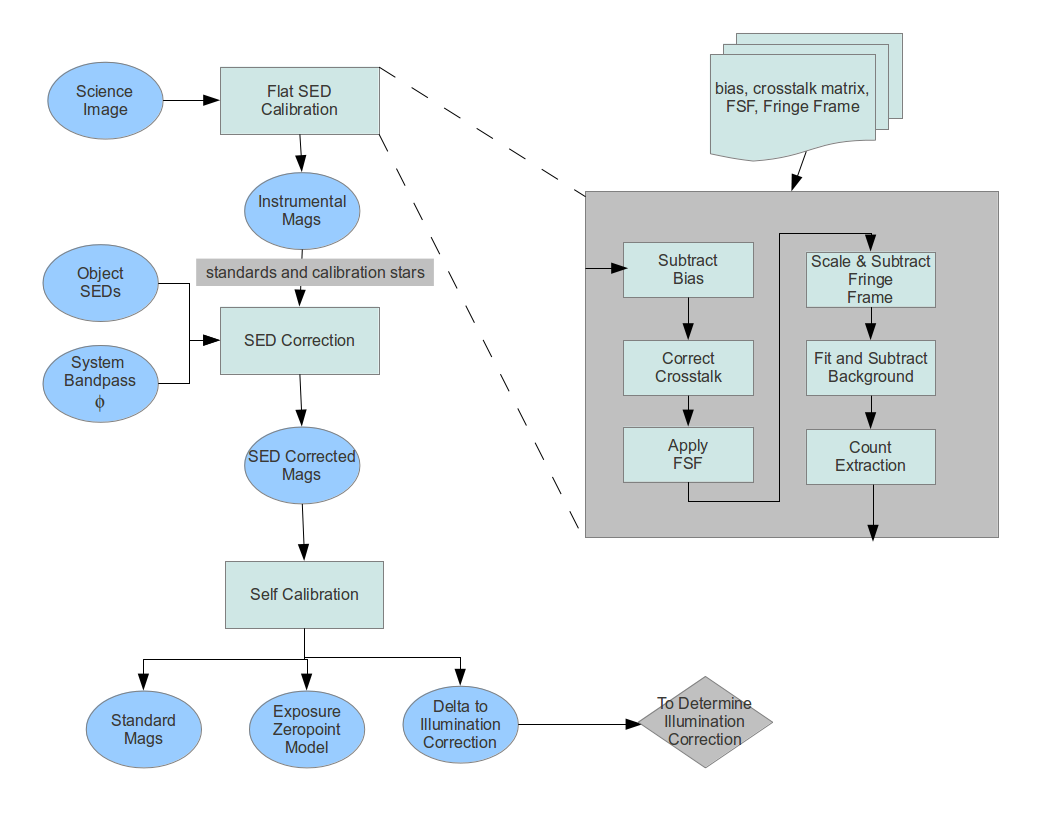
\includegraphics[width=6.5in]{CalibDataProdSchematic1}
\caption{ {\small {\bf The overall flow of the Data Release photometric
      calibration process.} The process consists of three main steps.  In the first, Flat SED Calibration, science image pixels are processed to instrumental magnitudes as if all calibration object SEDs were flat ($F_{\nu} = const$).  The second step, SED Correction, corrects the flat SED object counts to account for the real system bandpass and calibration object SEDs, generating corrected magnitudes.  The final step, Self Calibration, solves a least squares system in the SED corrected magnitudes to yield the standard magnitudes for the calibration objects and a spatially dependent zeropoint correction for each exposure.   Additionally, corrections to the illumination correction are calculated, for use in "Determine Illumination Correction" (Figure \ref{fig:overview_flowchart2}).  Note that SED Correction and Self Calibration are performed only for calibration objects.  General science objects are calibrated later, using the data products from the calibration process (Figure \ref{fig:overview_flowchart4}) }
\label{fig:overview_flowchart1} }
\end{minipage}
}
\end{figure}

\begin{figure}[htbp]
\centering
\fbox{
\begin{minipage}{6.5in}
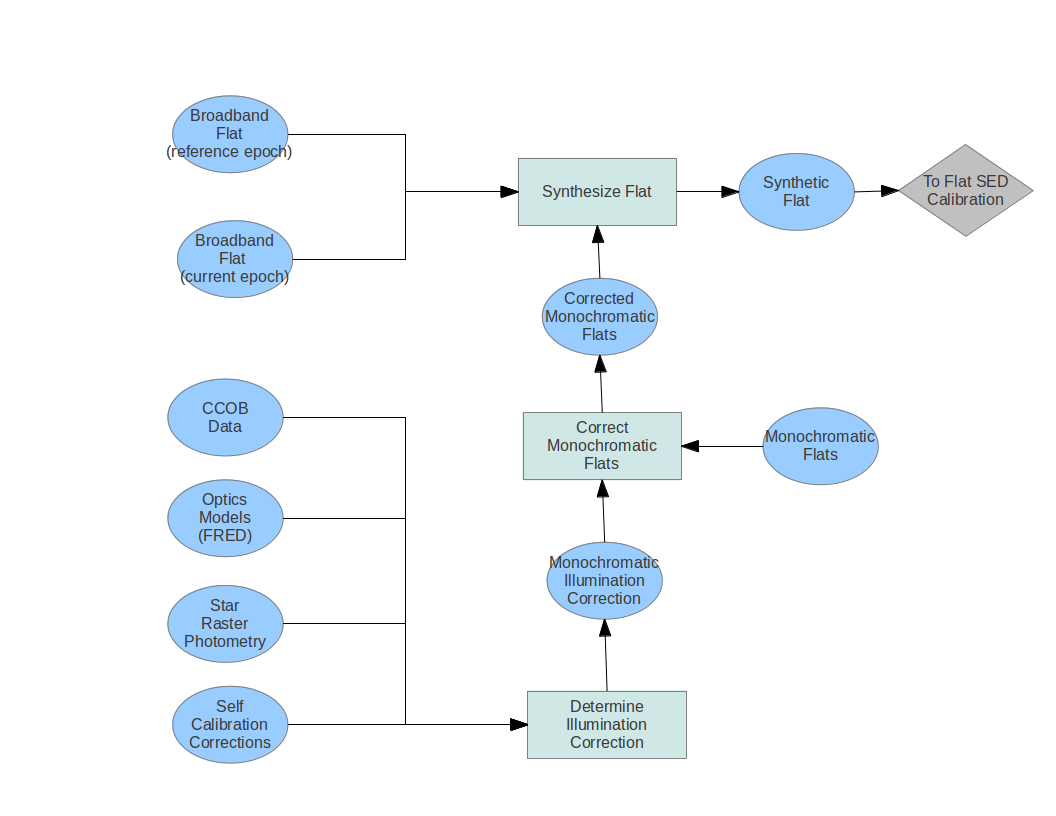
\includegraphics[width=6.5in]{CalibDataProdSchematic2}
\caption{ {\small {\bf Flat SED Flat Determination.} Determination of the flat SED flat (FSF) is of central importance.  The initial step in the calibration process treats all objects as if their SED were flat.  This is consistent only if the flatfield is that for a flat SED, as transmitted through a reference atmosphere.  Since the illumination source for the actual broadband flat does not have the required SED, we cannot use it directly.  Instead, we synthesize the required flat from the monochromatic flats.  These flats as measured are contaminated by light which arrives from paths other than the direct path, such as ghosting.  These effects are taken out by the illumination correction.  Additionally, the flats must be corrected for the nonuniform pixel solid angle on the sky. Finally, the monochromatic flats are taken relatively infrequently, and will not reflect changes on shorter timescales, such as the appearance of new dust particles.  We account for this by multiplying the synthesized FSF by the ratio of two broadband flats, one at the current epoch and one at the reference epoch, when the monochromatic flats were gathered.}
\label{fig:overview_flowchart2} }
\end{minipage}
}
\end{figure}

\begin{figure}[htbp]
\centering
\fbox{
\begin{minipage}{6.5in}
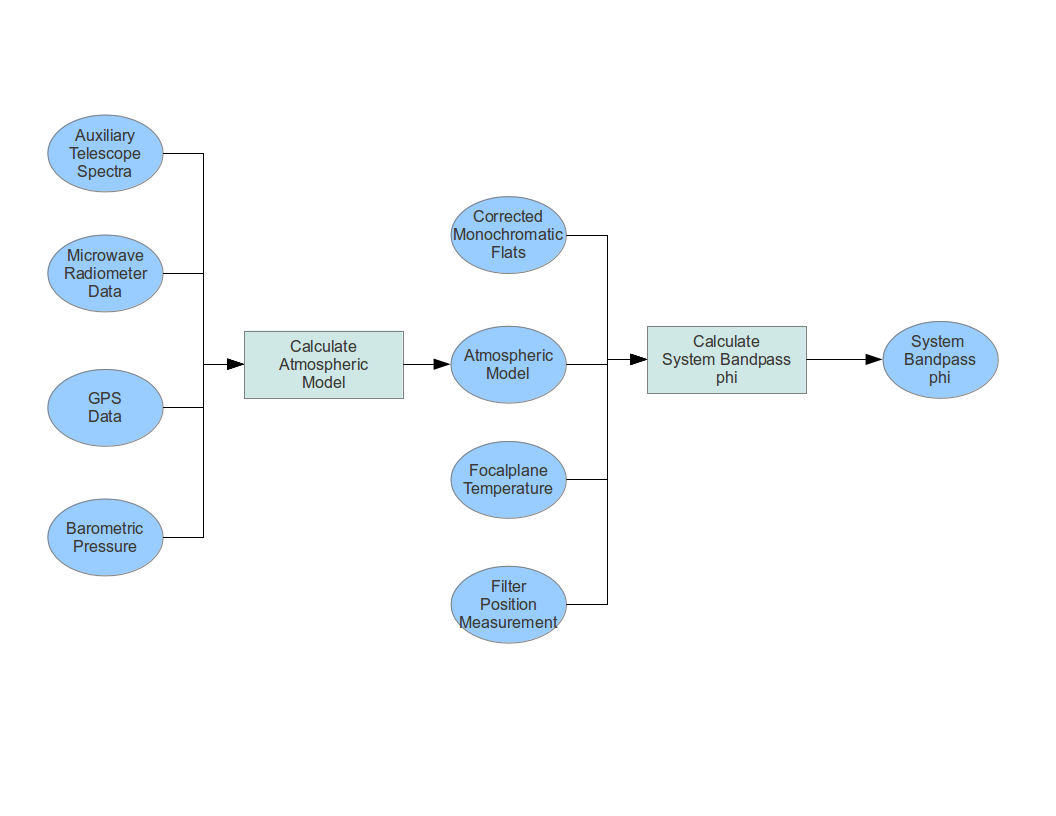
\includegraphics[width=6.5in]{CalibDataProdSchematic3}
\caption{ {\small {\bf System Bandpass Determination.} The system bandpass, $\phi$, is determined for every exposure, and is a major output of the calibration process.  It is the normalized product of the atmospheric bandpass and that of the telescope/camera system.  The atmospheric bandpass is determined by fitting an atmospheric model to a set of measured atmospheric data.  The bandpass of the telescope/camera system is measured by the corrected monochromatic flats, modified by current data from the camera system, principally focalplane temperature and the filter position. }
\label{fig:overview_flowchart3} }
\end{minipage}
}
\end{figure}

\begin{figure}[htbp]
\centering
\fbox{
\begin{minipage}{6.5in}
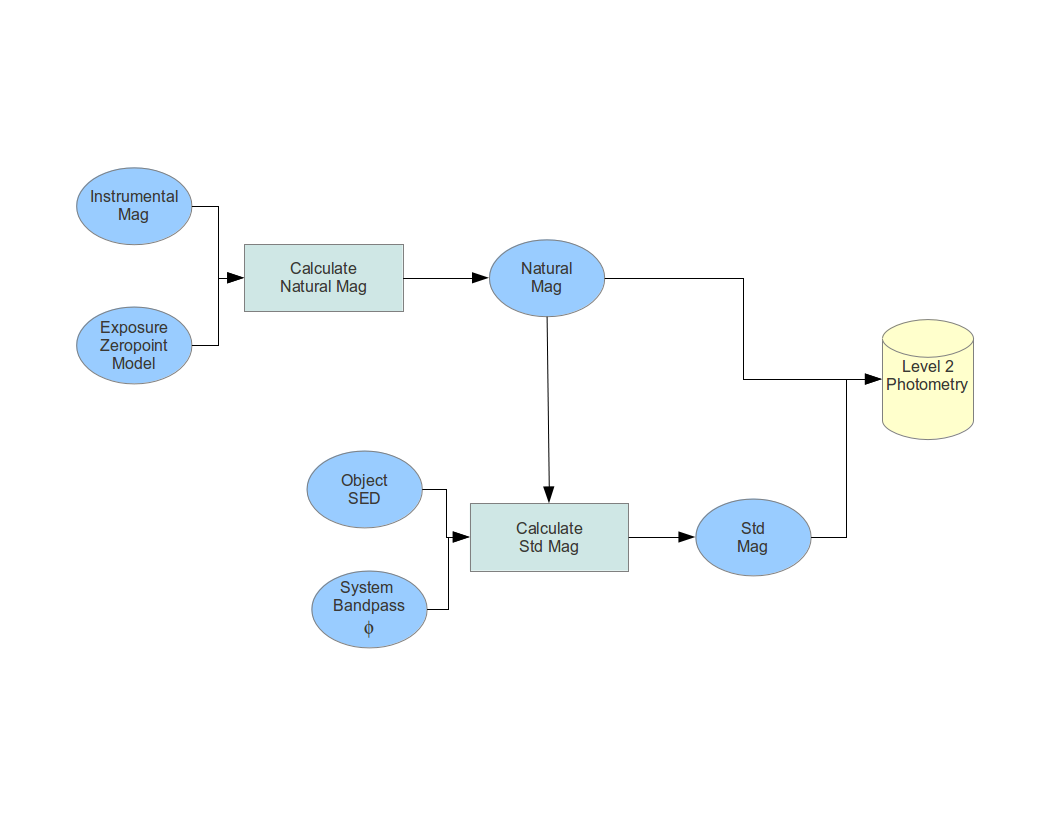
\includegraphics[width=6.5in]{CalibDataProdSchematic4}
\caption{ {\small {\bf Science Object Calibration.}  Photometric calibration for science objects takes place in two stages.  In the first, the natural magnitudes are calculated, using the zeropoint model for each exposure.  These are stored in the Level 2 databases.  The second, optional, stage, relies on knowledge of the object SEDs, which is an external input to the system, supplied by the user.   The object SED, in conjunction with the system bandpass, $\phi$, allows standard magnitudes to be calculated.  These are considered a Level 3 data product }
\label{fig:overview_flowchart4} }
\end{minipage}
}
\end{figure}

\clearpage

\begin{figure}[htbp]
\centering
\fbox{
\begin{minipage}{6.5in}
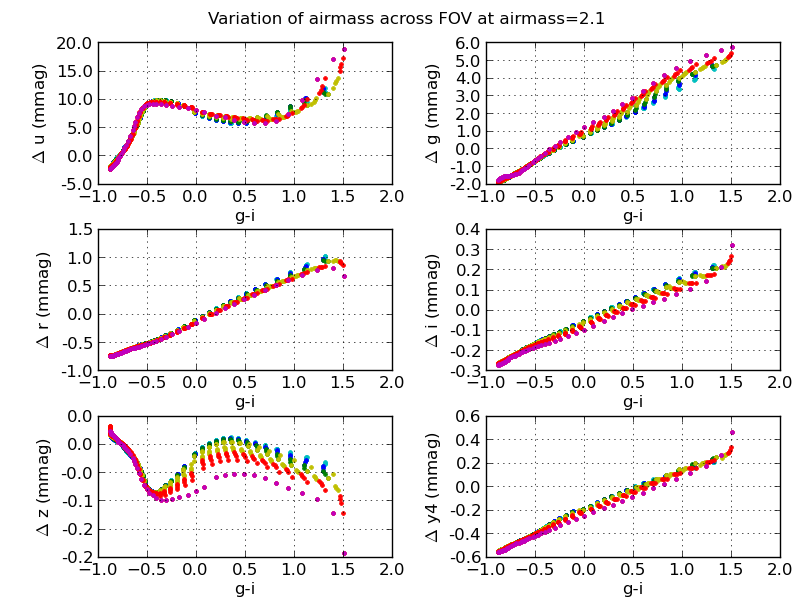
\includegraphics[width=6in]{AtmoFigs/AirmassAcrossFOV.png}
\caption{ {Effect on natural magnitudes of Kurucz stars from airmass variation across the field when the airmass at
field center is 2.1}.
\label{fig:dmag_fov} }
\end{minipage}
}
\end{figure}

\begin{figure}[htbp]
\centering
\fbox{
\begin{minipage}{6.5in}
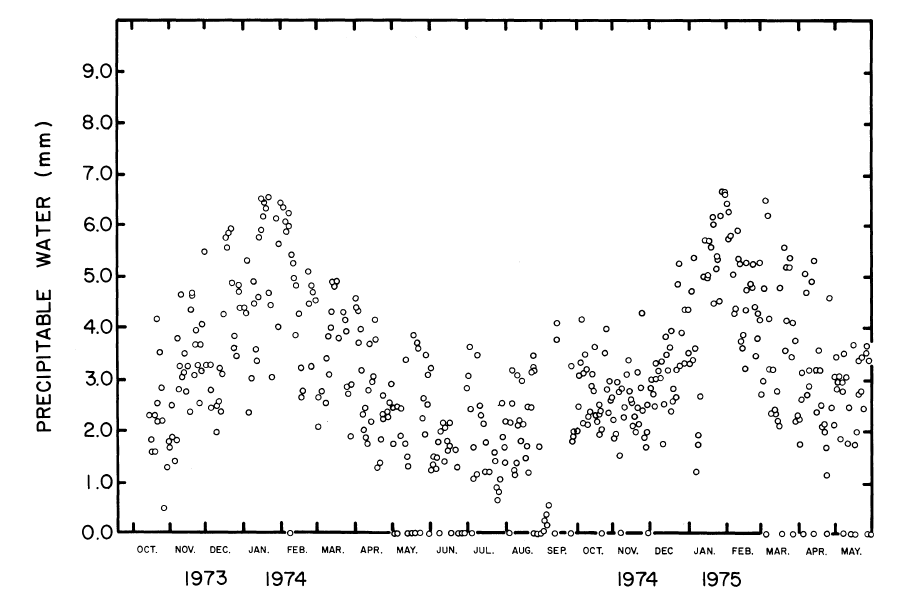
\includegraphics[width=6in]{AtmoFigs/CTIO_PWV}
\caption{ {Three years of PWV measured at CTIO (\citep{Hansen1975}), based on the depth of the 1.87 $\mu m$ line to the
Solar continuum at 1.65 $\mu m$}.
\label{fig:CTIO_PWV} }
\end{minipage}
}
\end{figure}

\begin{figure}[htbp]
\centering
\fbox{
\begin{minipage}{6.5in}
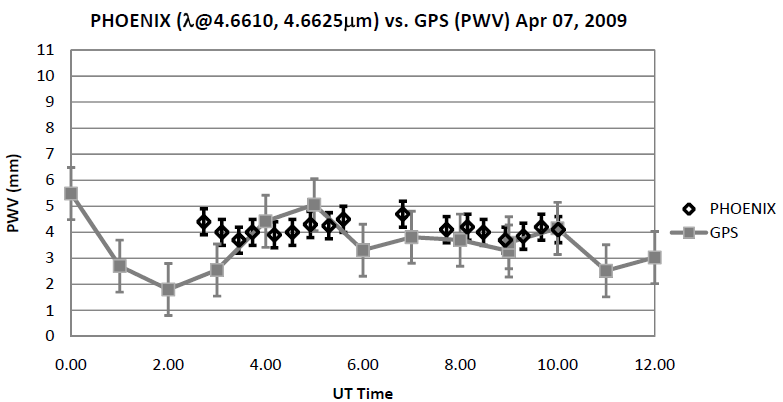
\includegraphics[width=6in]{AtmoFigs/GeminiPWV}
\caption{ {PWV measured on a single day at Gemini S \citep{Radomski2010}.  Two
techniques were used, GPS and Phoenix, an IR spectrograph, and the
data are in good agreement.  Note the decline of approximately 4 mm
over a period of two hours.  This is a case where use of a single
average atmosphere for a whole night would give poor results,
especially in the y-band.}
\label{fig:GeminiPWV} }
\end{minipage}
}
\end{figure}

\begin{figure}[htbp]
\centering
\fbox{
\begin{minipage}{6.5in}
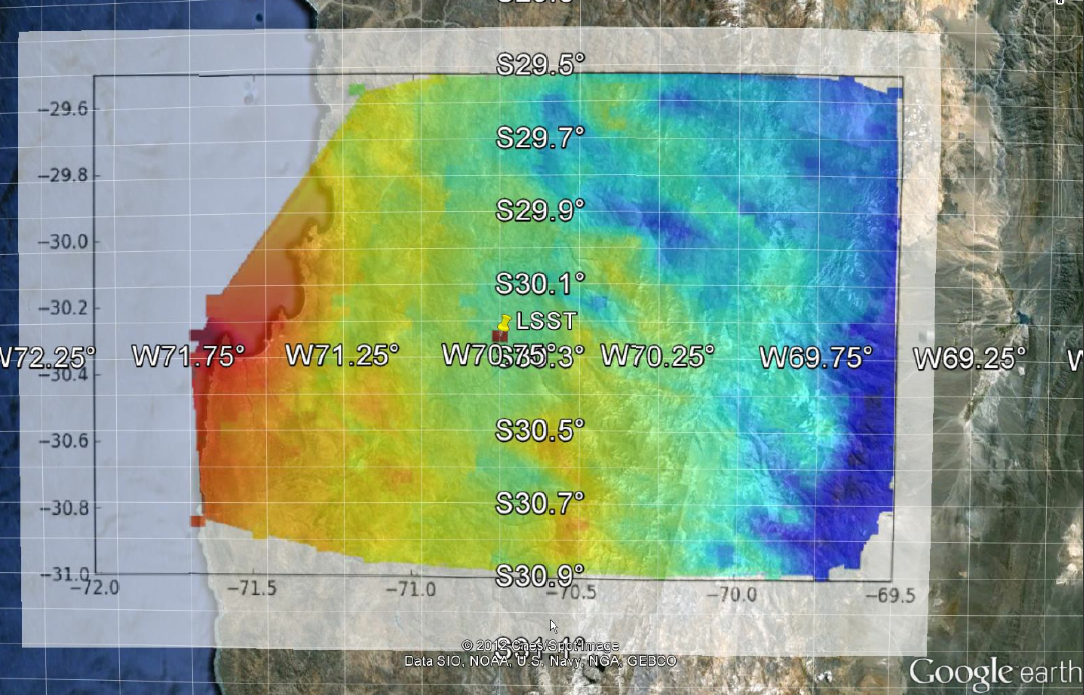
\includegraphics[width=6in]{AtmoFigs/PWV_satellite_2}
\caption{ {PWV measurement from the MODIS satellite at one time in the region
around Cerro Pachon.   The color scale ranges from 4.3 mm (blue) to 7.6 mm (dark red). Note the strong E-W gradient in PWV.}
\label{fig:PWV_satellite} }
\end{minipage}
}
\end{figure}

\begin{figure}[htbp]
\centering
\fbox{
\begin{minipage}{6.5in}
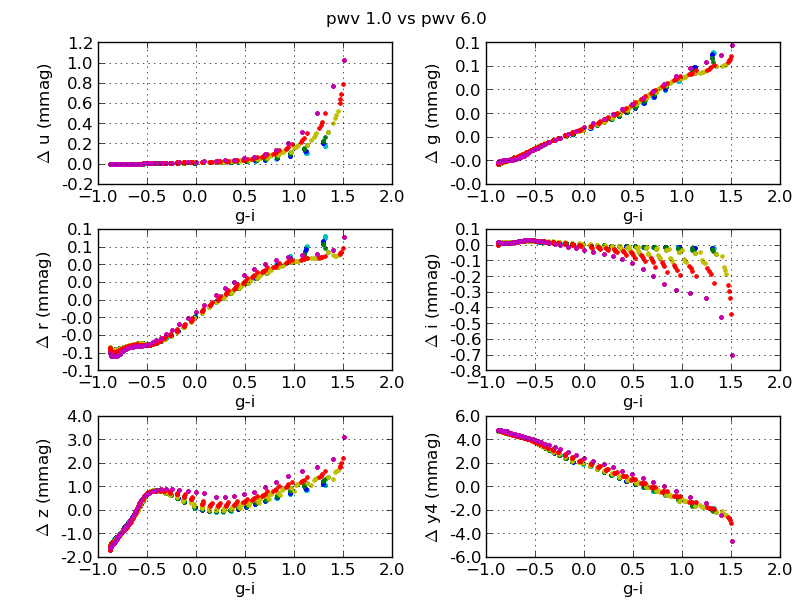
\includegraphics[width=6in]{AtmoFigs/KuruczPwv1_vs_6.png}
\caption{ {The effects of varying $\phi$ due to change in PWV from 1mm to 6mm -
about the range observed at Cerro Pachon.  The SEDs are for Kurucz
stars at varying temperatures and metallicities.}
\label{fig:KuruczPWV} }
\end{minipage}
}
\end{figure}

\begin{figure}[htbp]
\centering
\fbox{
\begin{minipage}{6.5in}
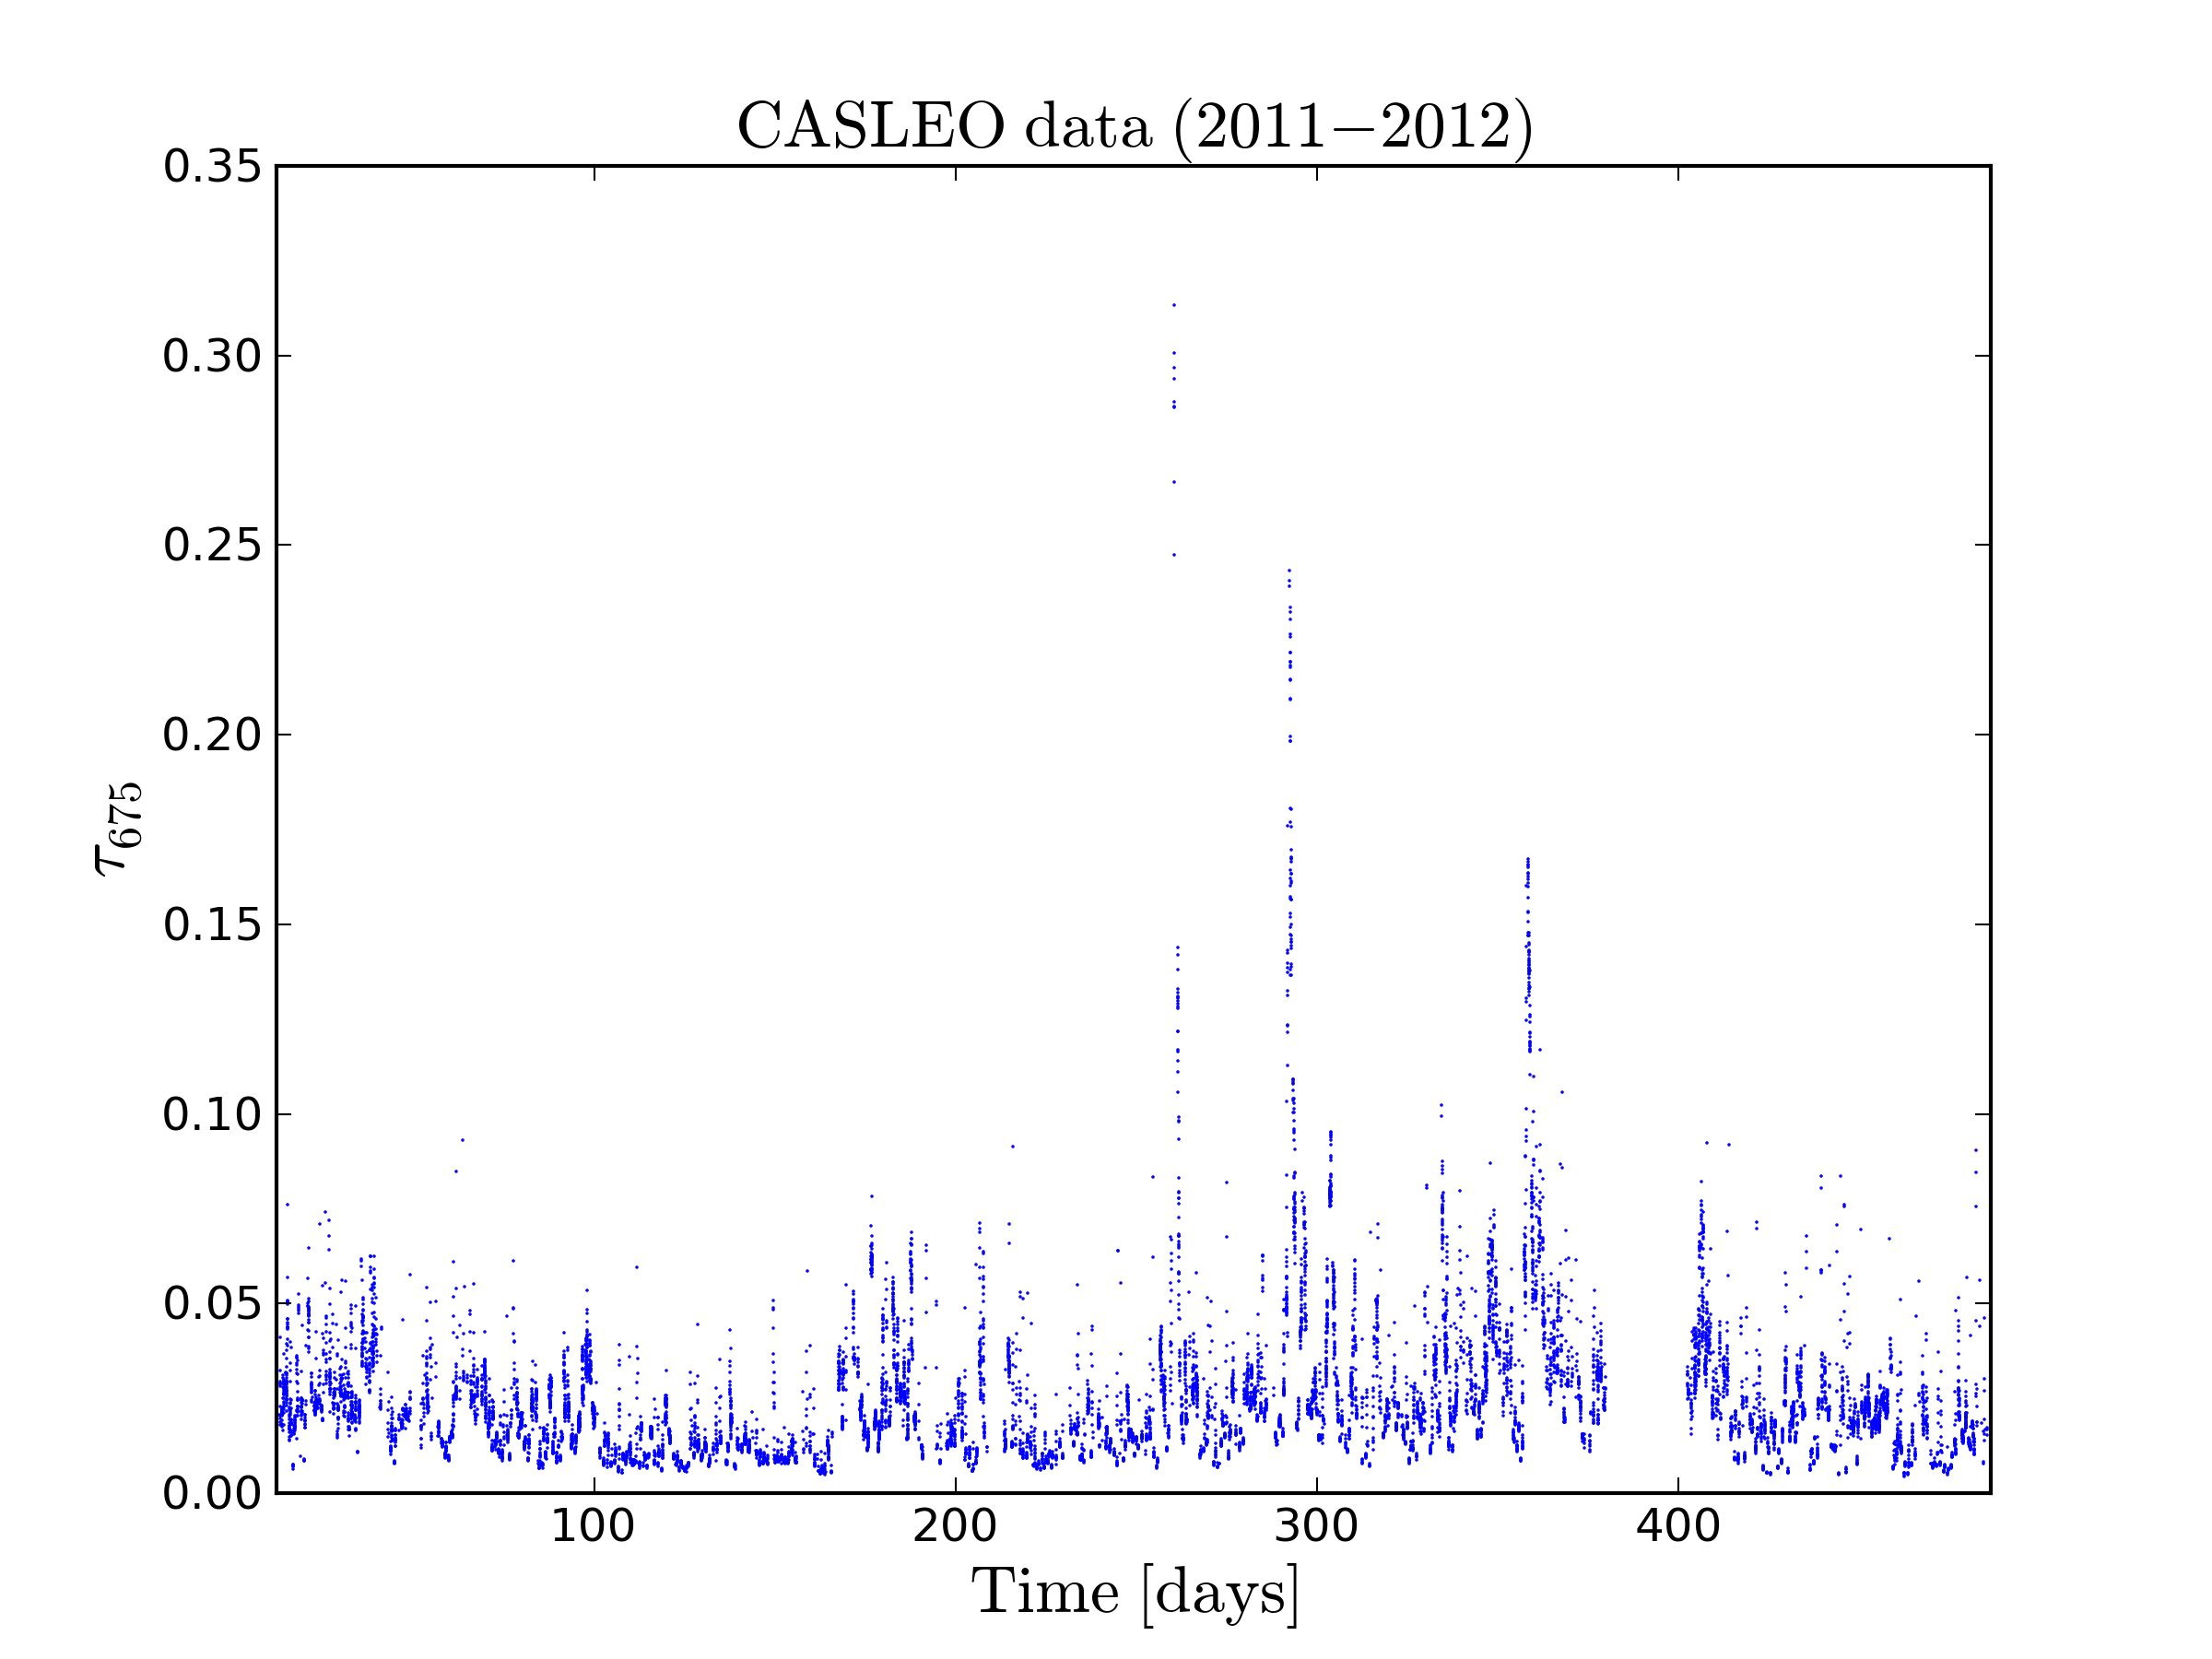
\includegraphics[width=6in]{AtmoFigs/aer_casleo.png}
\caption{ {Varying aersol optical depth at CASLEO, El Leoncito, Argentina.  The site elevation at 2550m is similar to CP.}
\label{fig:CASLEO} }
\end{minipage}
}
\end{figure}

\begin{figure}[htbp]
\centering
\fbox{
\begin{minipage}{6.5in}
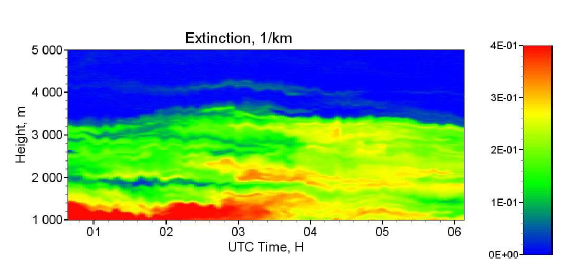
\includegraphics[width=6in]{AtmoFigs/AerosolVar}
\caption{ {Lidar measurements of aerosol extinction at 355nm over a single night
near Greenbelt, MD \citep{Veselovskii2013}.  Cerro Pachon is, of
course, a different environment, and is at an altitude of 2700m, removing
much of the variability.  Even above that altitude, however,
significant variation on rapid time scales remains.}
\label{fig:AerosolVar} }
\end{minipage}
}
\end{figure}


\begin{figure}[htbp]
\centering
\fbox{
\begin{minipage}{6.5in}
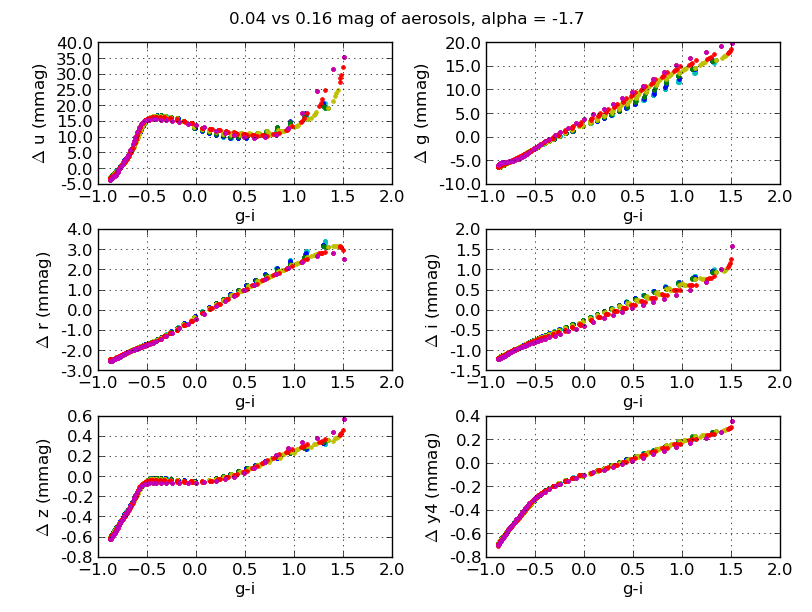
\includegraphics[width=6in]{AtmoFigs/KuruczAerosol_04vs16.png}
\caption{ {Effect on natural magnitude of Kurucz stars from varying the aerosol optical depth from 0.04mag to 0.16mag} 
\label{fig:KuruczAerosol} }
\end{minipage}
}
\end{figure}

\begin{figure}[htbp]
\centering
\fbox{
\begin{minipage}{6.5in}
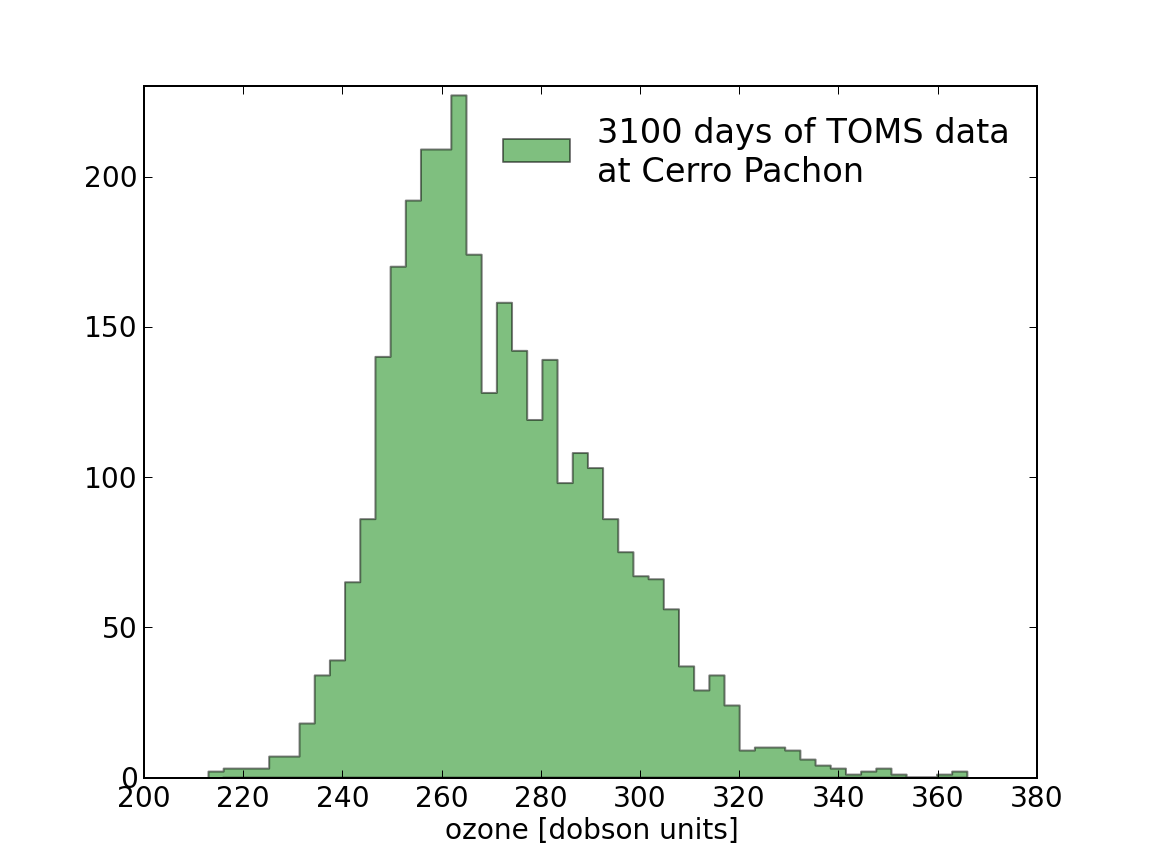
\includegraphics[width=6in]{AtmoFigs/hist_ozone9Y.png}
\caption{ {Variability of ozone column depth at Cerro Pachon from the TOMS satellite instrument} 
\label{fig:O3atCP} }
\end{minipage}
}
\end{figure}

\begin{figure}[htbp]
\centering
\fbox{
\begin{minipage}{6.5in}
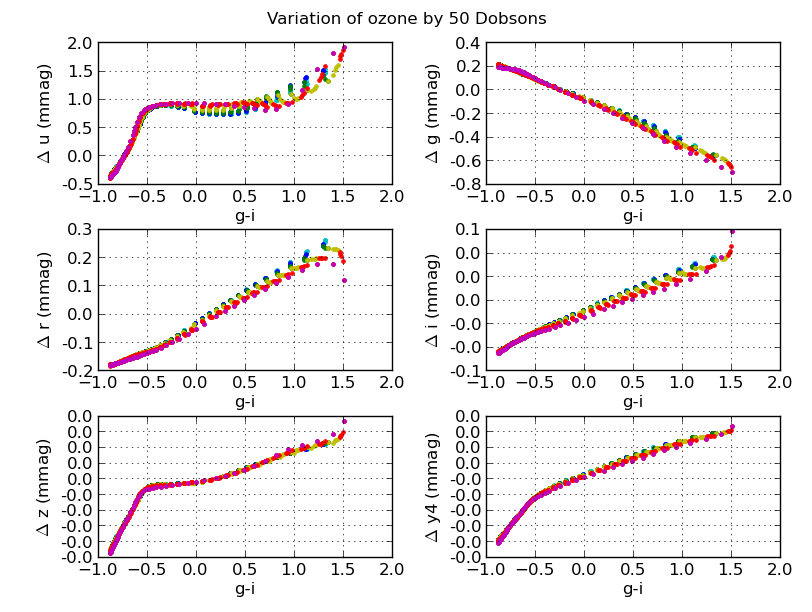
\includegraphics[width=6in]{AtmoFigs/KuruczO3_50dobs.png}
\caption{ {Effect on natural magnitude of Kurucz stars from varying the ozone column by 50 Dobson units} 
\label{fig:KuruczO3} }
\end{minipage}
}
\end{figure}

\begin{figure}[htbp]
\centering
\fbox{
\begin{minipage}{6.5in}
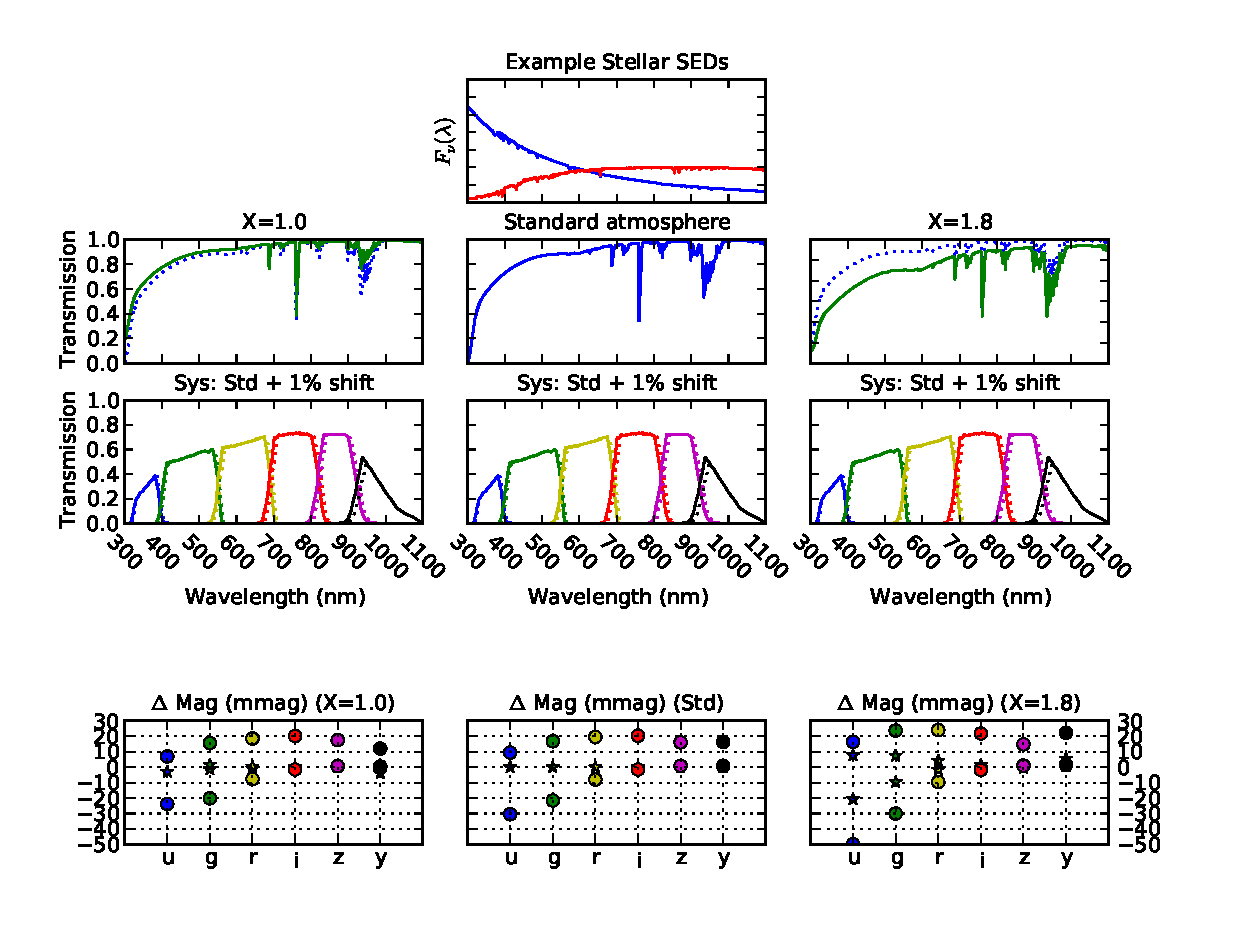
\includegraphics[width=6in]{delta_mags}
\caption{ {\small {\bf $\Delta m_b^{obs}$ due to variations in
hardware and atmospheric bandpass shape.} Two main sequence Kurucz model
stars, one blue (35000 K, approximately O type) and one red (6000 K
approximately G type), were used to generate
natural magnitudes (see 
Eqn~\ref{eqn:natmag}) using three different atmospheric transmission
profiles and two different hardware transmission profiles. The stellar
flux profiles are shown in the top center panel, while the atmospheric
transmission functions ($S^{atm}(\lambda)$) are shown across the
second row and the two hardware transmission profiles
($S_b^{sys}(\lambda)$) are duplicated across the third row. The
atmospheric transmission profiles correspond to an airmass X=1.0, 1.2
and 1.8 (from left to right), with variable atmospheric absorption
components. The X=1.0 atmosphere is very similar but not
identical to the current LSST default X=1.2 atmosphere throughput
curve, which is used as `standard' here. The hardware transmission
profiles consist of a `standard' profile (matching the LSST current
expected values) and version where the filter throughputs have been
shifted by 1\% of the effective wavelength of each filter (consistent
with the shift expected near the spatial edge of each filter). The final row
demonstrates the changes in observed magnitudes produced by the X=1.0,
`standard' and X=1.8 atmospheres (left to right, respectively),
combined with both the `standard' hardware transmission (represented by
the star points) and the +1\% shifted hardware transmission (represented
by the filled circles) for both the red and blue stars. The exact
differences in magnitudes resulting from this calculation are listed in
Table~\ref{tab:delta_mags}. }
\label{fig:delta_mags} }
\end{minipage}
}
\end{figure}

\begin{center}
\begin{table}[htb]
\caption{{\bf $\Delta m_b^{obs}$ due to variations in system and atmospheric
 bandpass shape (see also Fig~\ref{fig:delta_mags}). The first two
rows show the baseline (`standard') magnitude of the star. All other rows show the 
{\it change} in magnitude (in mmag) due to the variations listed at
left. Any value larger than 5~mmag would be larger than the RMS
scatter allowed by the SRD. {\it TODO color-code values larger than 5 mmag}} }
\begin{tabular}{l l | c c c c c c}
Bandpass & star &  $u$ (mag) & $g$ & $r$ & $i$ & $z$ & $y$ \\ \hline
Std (X=1.2) atm, std sys  &  red & 21.472 & 20.378 & 20.000 & 19.911 & 19.913 & 19.913 \\
Std (X=1.2) atm, std sys  &  blue & 19.102 & 19.503 & 20.000 & 20.378 & 20.672 & 20.886 \\ \hline \hline
 & & $\Delta u$ (mmag) & $\Delta g$  & $\Delta r$  & $\Delta i$ & $\Delta z$  & $\Delta y$ \\ \hline
Std (X=1.2), +1\% sys shift & red  & -31 & -22 & -8 & -2 & 1 & 1 \\
Std (X=1.2), +1\% sys shift & blue  & 9 & 17 & 20 & 20 & 16 & 16 \\ \hline
X=1.0, std sys & red  & 7 & 2 & 0 & 0 & -0 & -1 \\
X=1.0, std sys & blue  & -3 & -1 & -1 & -0 & 1 & -4 \\ \hline
X=1.0, +1\% sys shift & red & -24 & -20 & -8 & -1 & 1 & 0 \\
X=1.0, +1\% sys shift & blue & 7 & 16 & 19 & 20 & 18 & 12 \\ \hline
X=1.8, std sys  & red & -21 & -10 & -2 & -0 & 0 & 1 \\
X=1.8, std sys  & blue & 8 & 8 & 4 & 2 & -1 & 6 \\ \hline
X=1.8, +1\% sys shift & red & -50 & -30 & -10 & -2 & 1 & 2 \\
X=1.8, +1\% sys shift & blue & 16 & 24 & 24 & 22 & 15 & 22 \\ \hline
\end{tabular}
\label{tab:delta_mags}
\end{table}
\end{center}

\clearpage

\begin{figure}[htbp]
\centering
\fbox{
\begin{minipage}{6.5in}
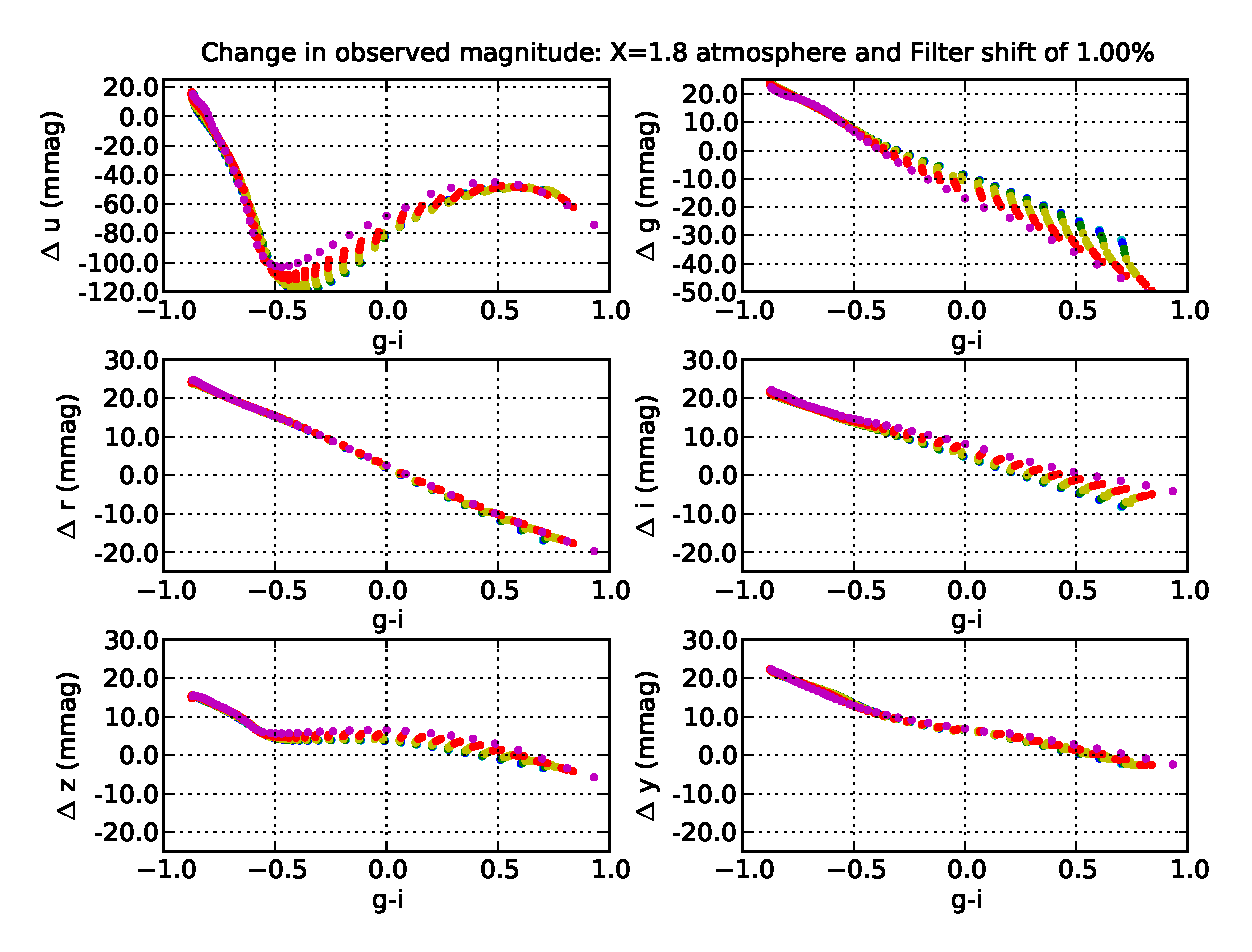
\includegraphics[width=6in]{delta_mags2}
\caption{ {\small {\bf $\Delta m_b^{obs}$ due to
a change in bandpass shape corresponding to a filter shift of $1\%$
and an $X=1.8$ atmosphere.} 850 Kurucz models with temperatures
between 5000K and 35000K and metallicity indexes between -5.0 and 1.0
(solar) were combined with a standard system response (standard
atmosphere and standard hardware bandpasses), then with a total system
response where the atmosphere was replaced by an X=1.8 atmosphere and
the filter component of the hardware transmission was shifted by 1\%
(as in Fig~\ref{fig:delta_mags}). The points in each plot are color-coded by
metallicity, in steps of 1 dex between -5.0 (blue) to 1.0 (magenta).  It can be seen that the
relationship between $\Delta m_b^{obs}$ and $g-i$ can be parameterized,
although generally not with a simple linear relationship. In some
cases (such as seen in the $\Delta u$ and $\Delta g$ panels),
calculating $\Delta m_b^{obs}$ to SRD levels may require more than a simple
$g-i$ color, but this is then primarily a function of metallicity
(which is possible to determine given the $u-g$ color in addition to
the $g-i$ information). }
\label{fig:delta_mags2} }
\end{minipage}
}
\end{figure}

\begin{figure}[htbp]
\centering
\fbox{
\begin{minipage}{6.5in}
\begin{tabular}{cc}
\subfloat[]{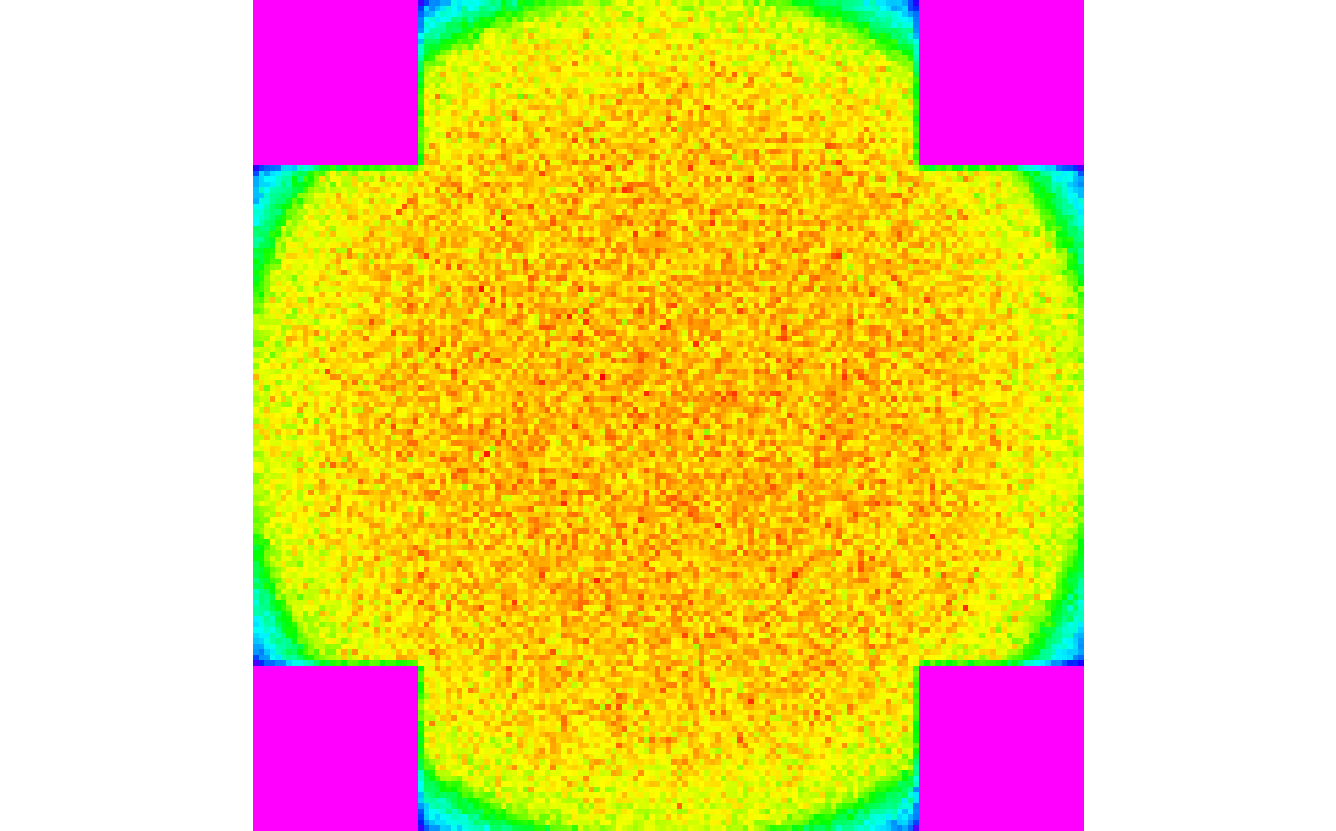
\includegraphics[width=3in]{IllumCorrFigs/monochromatic_360nm_direct.png}}
	& \subfloat[]{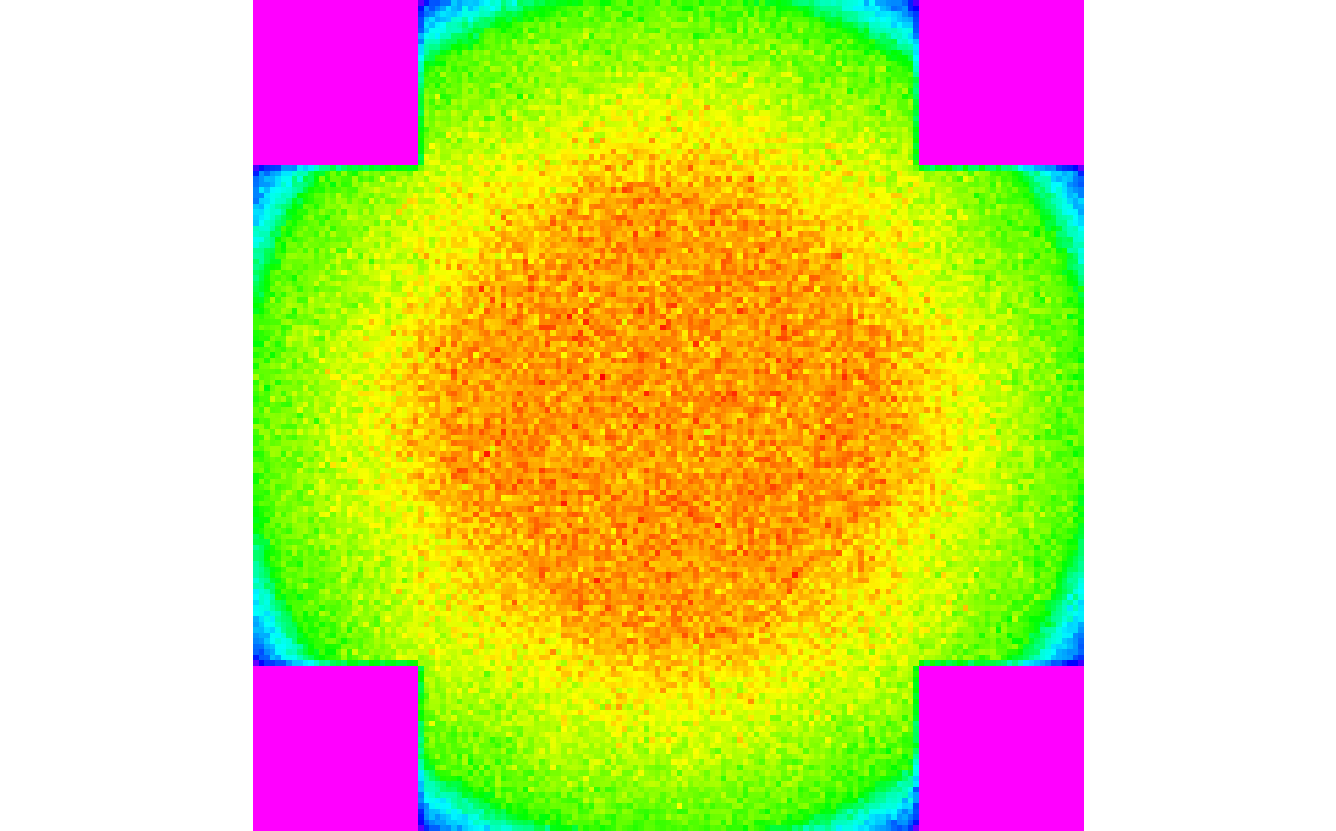
\includegraphics[width=3in]{IllumCorrFigs/monochromatic_360nm_total.png}} \\
\subfloat[]{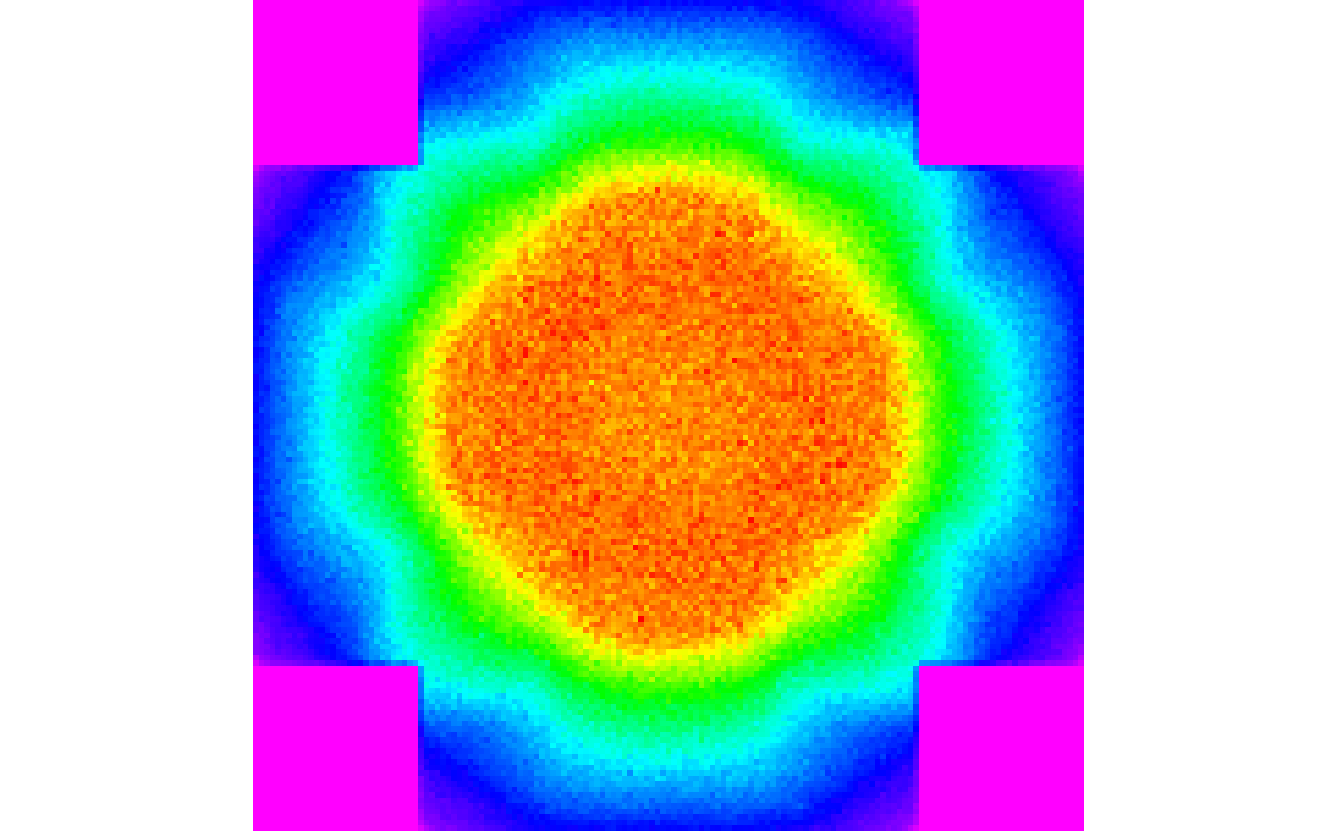
\includegraphics[width=3in]{IllumCorrFigs/monochromatic_360nm_ghost.png}}
	& \subfloat[]{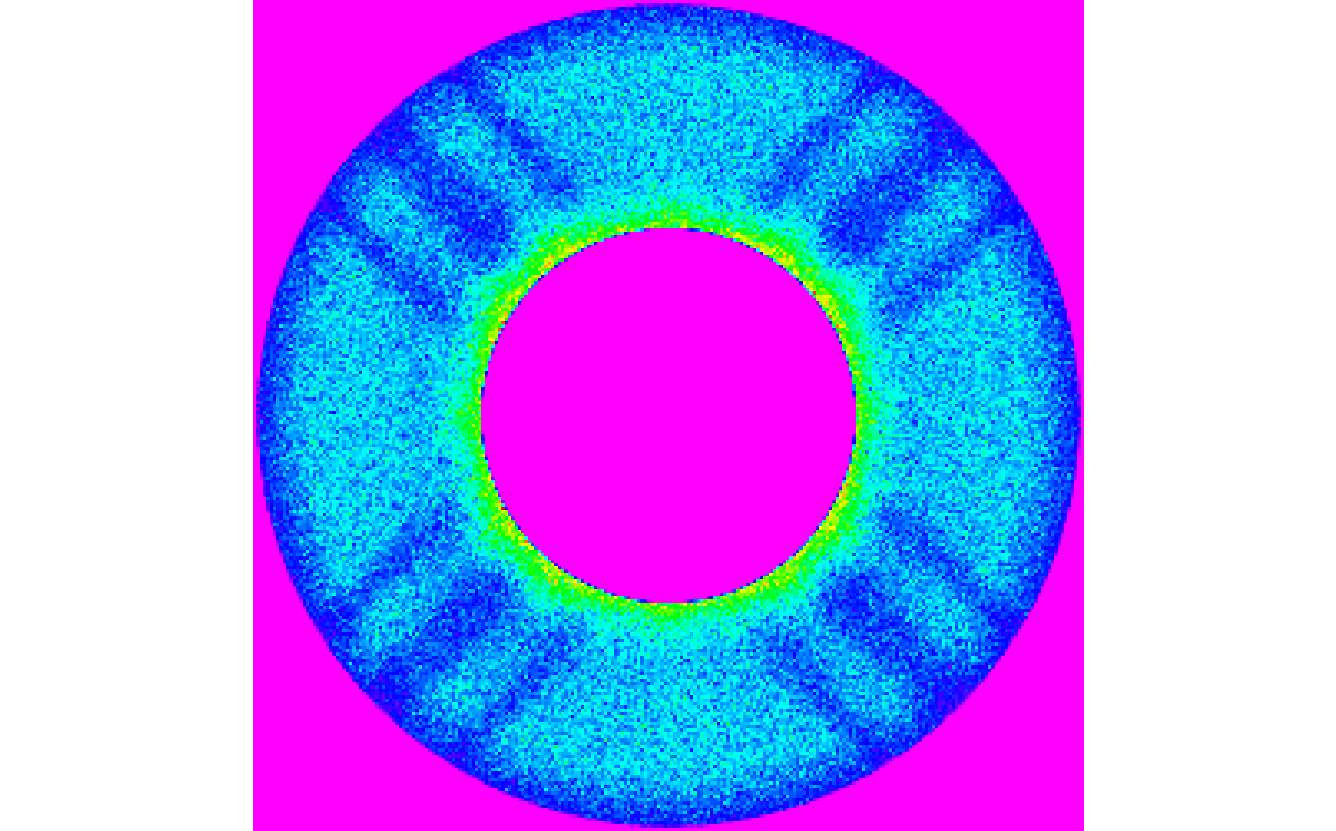
\includegraphics[width=3in]{IllumCorrFigs/monochromatic_360nm_screen.png}} \\
\end{tabular}	
\caption{ {FRED calculation of flat from monochromatically illuminated screen.  The u filter is in place, 
and the illuminating wavelength is 360nm, near the red limit of the filter.  (a) direct illumination
(b) total illumination (c) ghost illumination (d) screen illumination.  The illumination correction
is the ratio direct / total.} 
\label{fig:FRED360nm} }
\end{minipage}
}
\end{figure}

\begin{figure}[htbp]
\centering
\fbox{
\begin{minipage}{6.5in}
\begin{tabular}{cc}
\subfloat[]{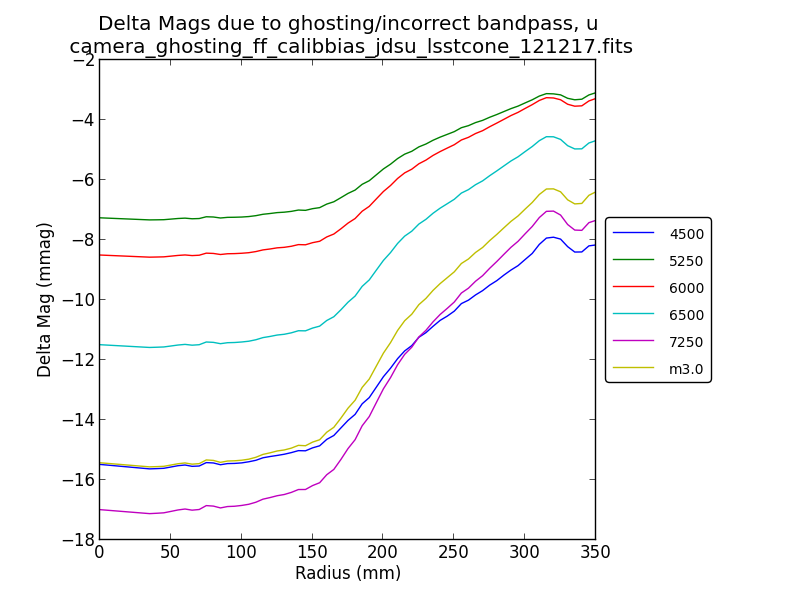
\includegraphics[width=3in]{IllumCorrFigs/camera_ghosting_ff_calibbias_jdsu_lsstcone_121217_u_ghosting.png}}
	& \subfloat[]{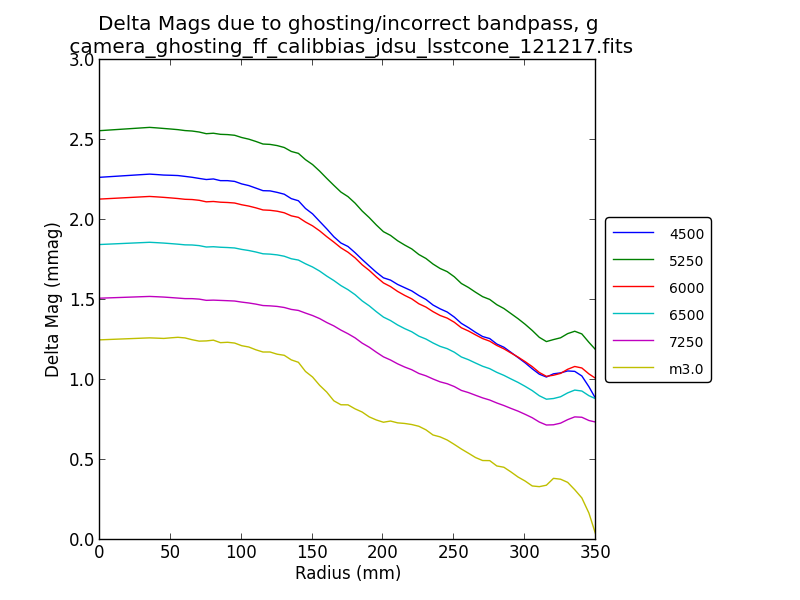
\includegraphics[width=3in]{IllumCorrFigs/camera_ghosting_ff_calibbias_jdsu_lsstcone_121217_g_ghosting.png}} \\ 
\subfloat[]{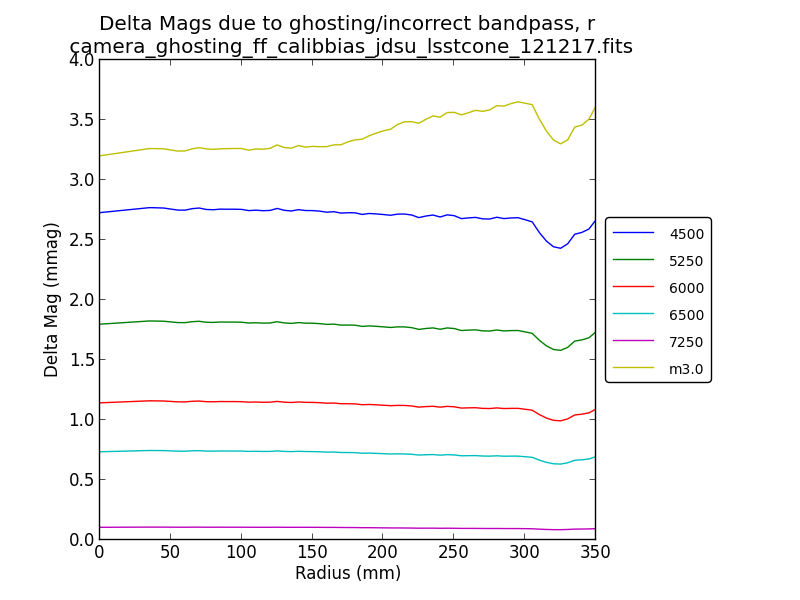
\includegraphics[width=3in]{IllumCorrFigs/camera_ghosting_ff_calibbias_jdsu_lsstcone_121217_r_ghosting.png}}
	& \subfloat[]{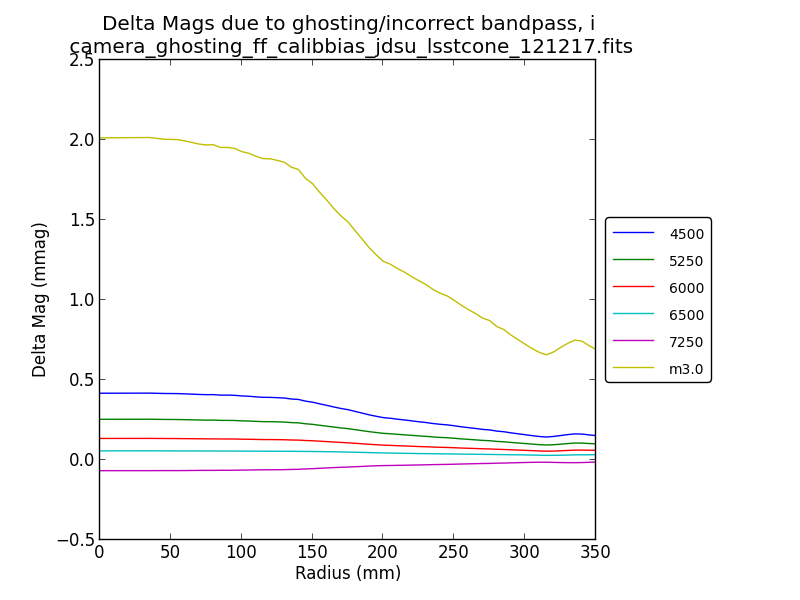
\includegraphics[width=3in]{IllumCorrFigs/camera_ghosting_ff_calibbias_jdsu_lsstcone_121217_i_ghosting.png}} \\
\subfloat[]{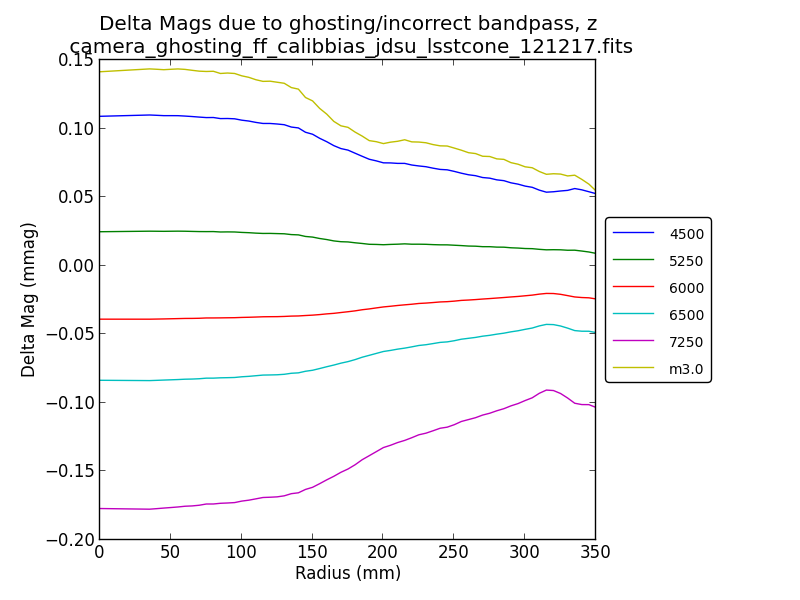
\includegraphics[width=3in]{IllumCorrFigs/camera_ghosting_ff_calibbias_jdsu_lsstcone_121217_z_ghosting.png}}
	& \subfloat[]{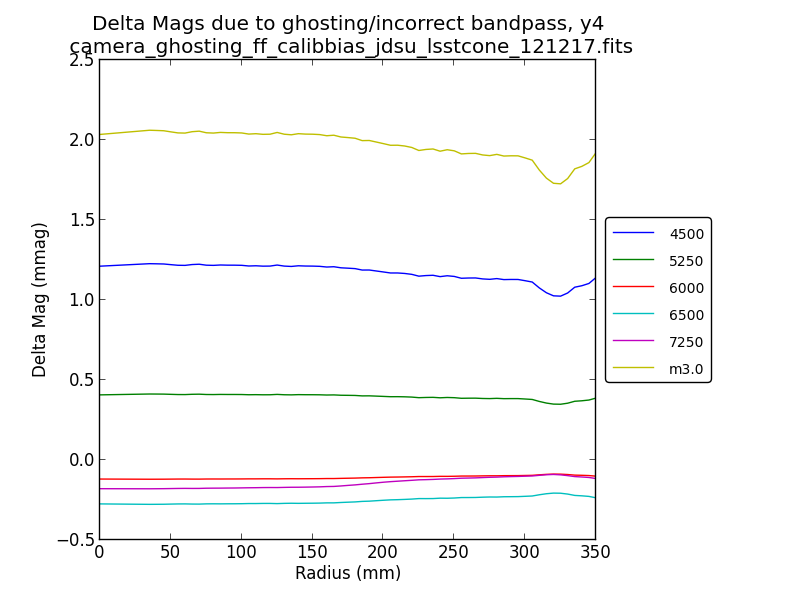
\includegraphics[width=3in]{IllumCorrFigs/camera_ghosting_ff_calibbias_jdsu_lsstcone_121217_y4_ghosting.png}} \\
\end{tabular}	
\caption{ {The effects of the illumination correction, as calculated by \citep{AndyR2013}, on the natural magnitudes of Kurucz stars
of varying temperatures.  All 6 LSST passbands are shown.} 
\label{fig:IllumCorrKurucz} }
\end{minipage}
}
\end{figure}

\begin{figure}[htbp]
\centering
\fbox{
\begin{minipage}{6.5in}
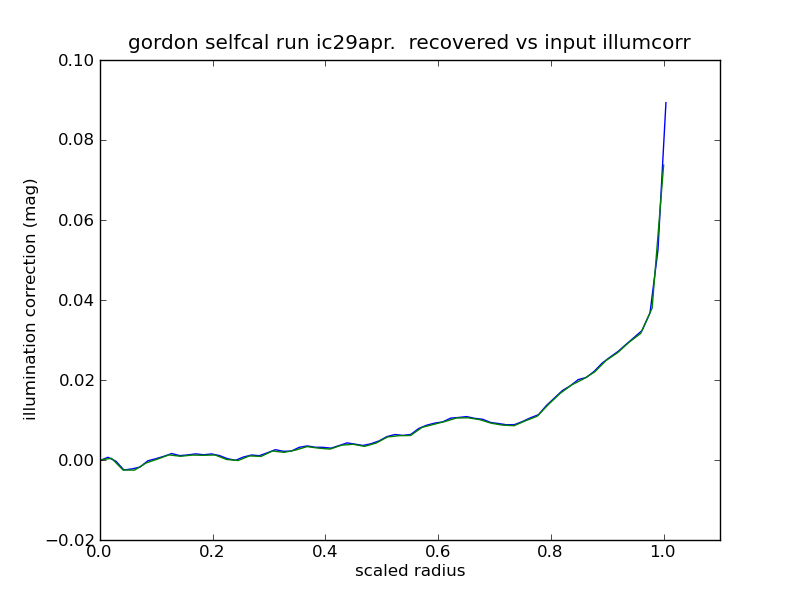
\includegraphics[width=6in]{IllumCorrFigs/fidic29apr_input_vs_recovered_ic.png}
\caption{ \small {Recovery of input broadband illumination correction by self calibration.  The input illumination 
correction was wavelength independent, but strongly dependent on radial position, as shown.   The recovered illumination
correction is essentially identical to that input.}
\label{fig:SelfCalIllumCorr} }
\end{minipage}
}
\end{figure}


\begin{figure}[htbp]
\centering
\fbox{
\begin{minipage}{6.5in}
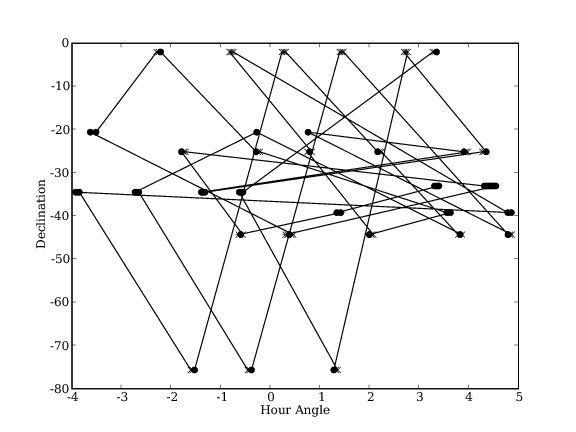
\includegraphics[width=6in]{AtmoFigs/burk0711/f5.png}
\caption{ {Pattern of observing atmospheric probe stars from \citep{Burke2010b}.  The Solid lines trace
the temporal order of the observations} 
\label{fig:BurkeObsPattern} }
\end{minipage}
}
\end{figure}

\begin{figure}[htbp]
\centering
\fbox{
\begin{minipage}{6.5in}
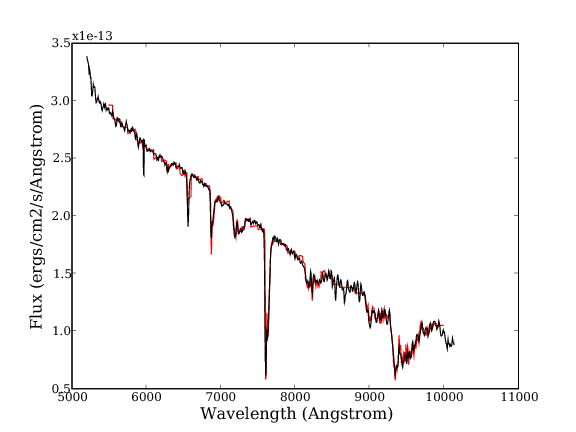
\includegraphics[width=6in]{AtmoFigs/burk0711/f3b.png}
\caption{ {Typical observed spectrum (black) and fit (red) from \citep{Burke2010b}} 
\label{fig:BurkeSpectrumFit} }
\end{minipage}
}
\end{figure}

\begin{figure}[htbp]
\centering
\fbox{
\begin{minipage}{6.5in}
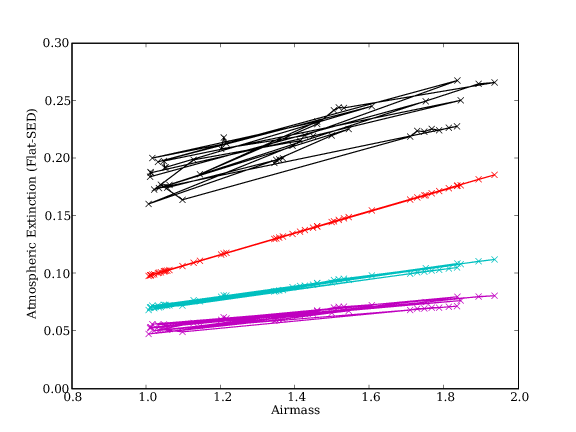
\includegraphics[width=6in]{AtmoFigs/burk0711/f10.png}
\caption{ {Non-gray atmospheric extinction from \citep{Burke2010b}.  Red is r-band, cyan is i-band,
magenta is z-band, black is y-band.} 
\label{fig:BurkeExtinction} }
\end{minipage}
}
\end{figure}
\begin{figure}[htbp]
\centering
\fbox{
\begin{minipage}{6.5in}
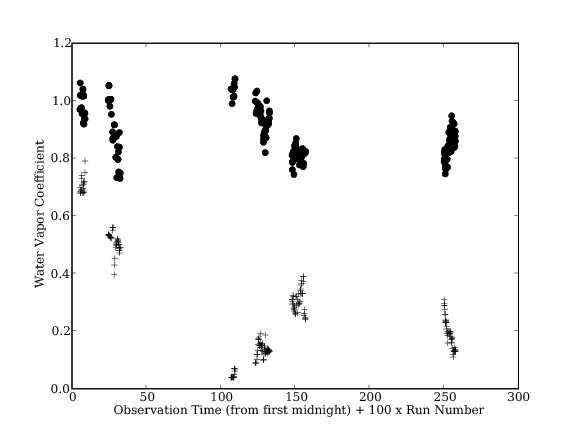
\includegraphics[width=6in]{AtmoFigs/burk0711/f7.png}
\caption{ {Fitted water vapor coefficient from \citep{Burke2010b}, expressed as a ratio to the standard value (filled circles).
Crosses are relative humidity from CTIO (changed scale). } 
\label{fig:BurkeWaterVapor} }
\end{minipage}
}
\end{figure}  

\clearpage

\begin{figure}
\centering
\fbox{
\begin{minipage}{6.5in}
\subfloat[\citet{Stubbs2010a} \label{diodeStubbs}]{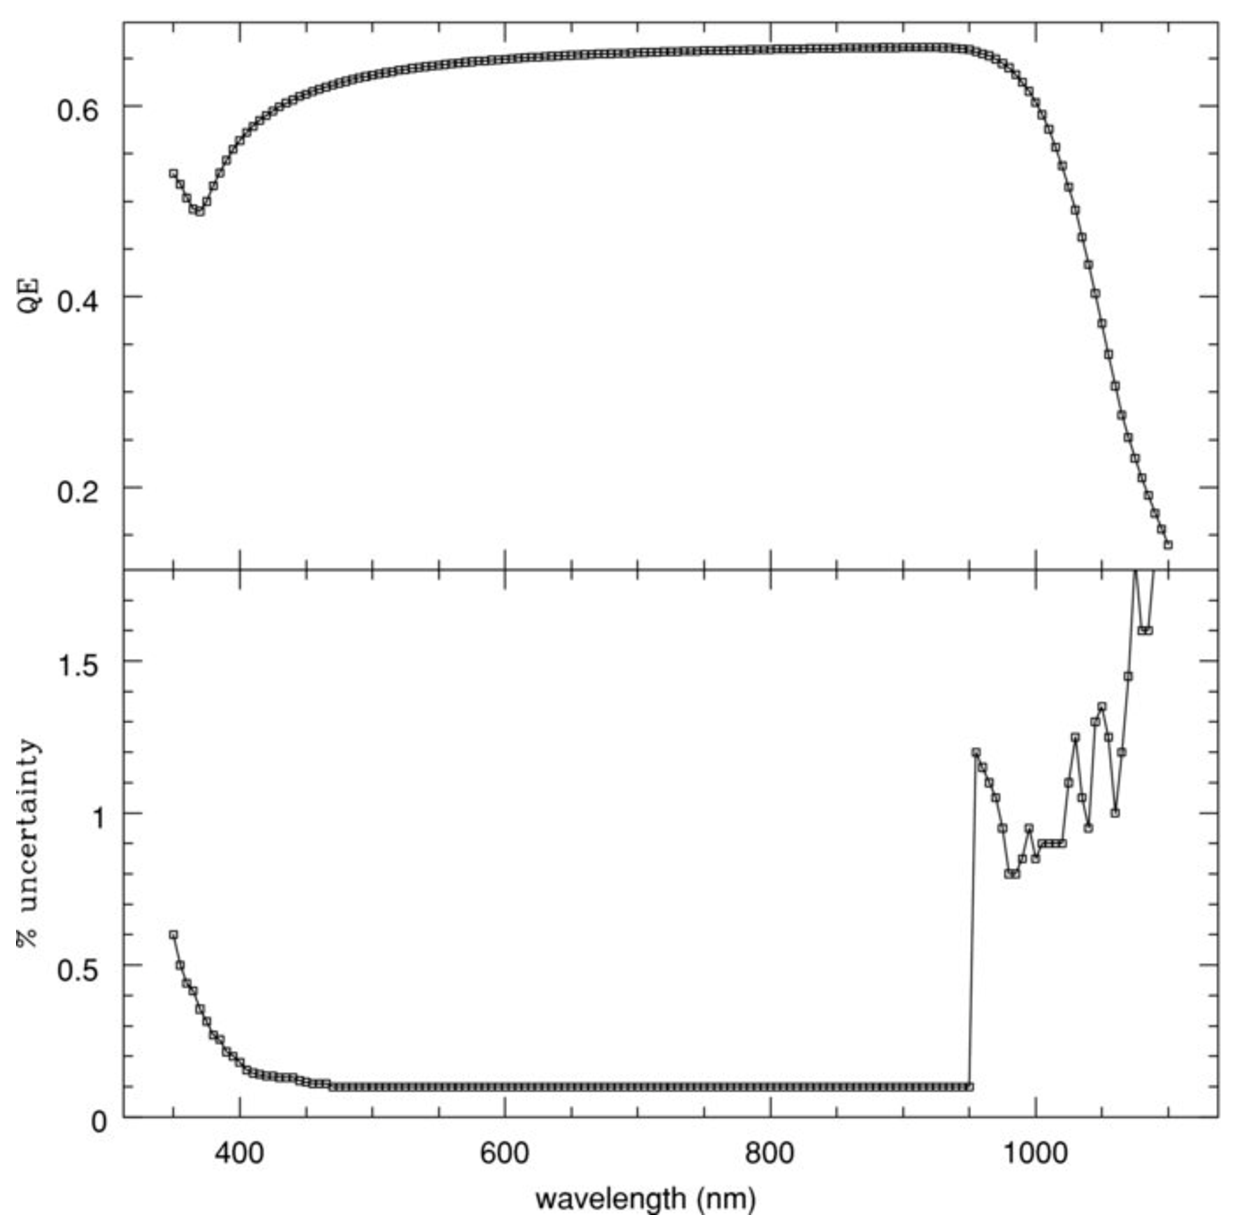
\includegraphics[width=3.5in]{NIST_diode}} \\
\subfloat[\citet{Eppeldauer09} \label{diodeEppel}]{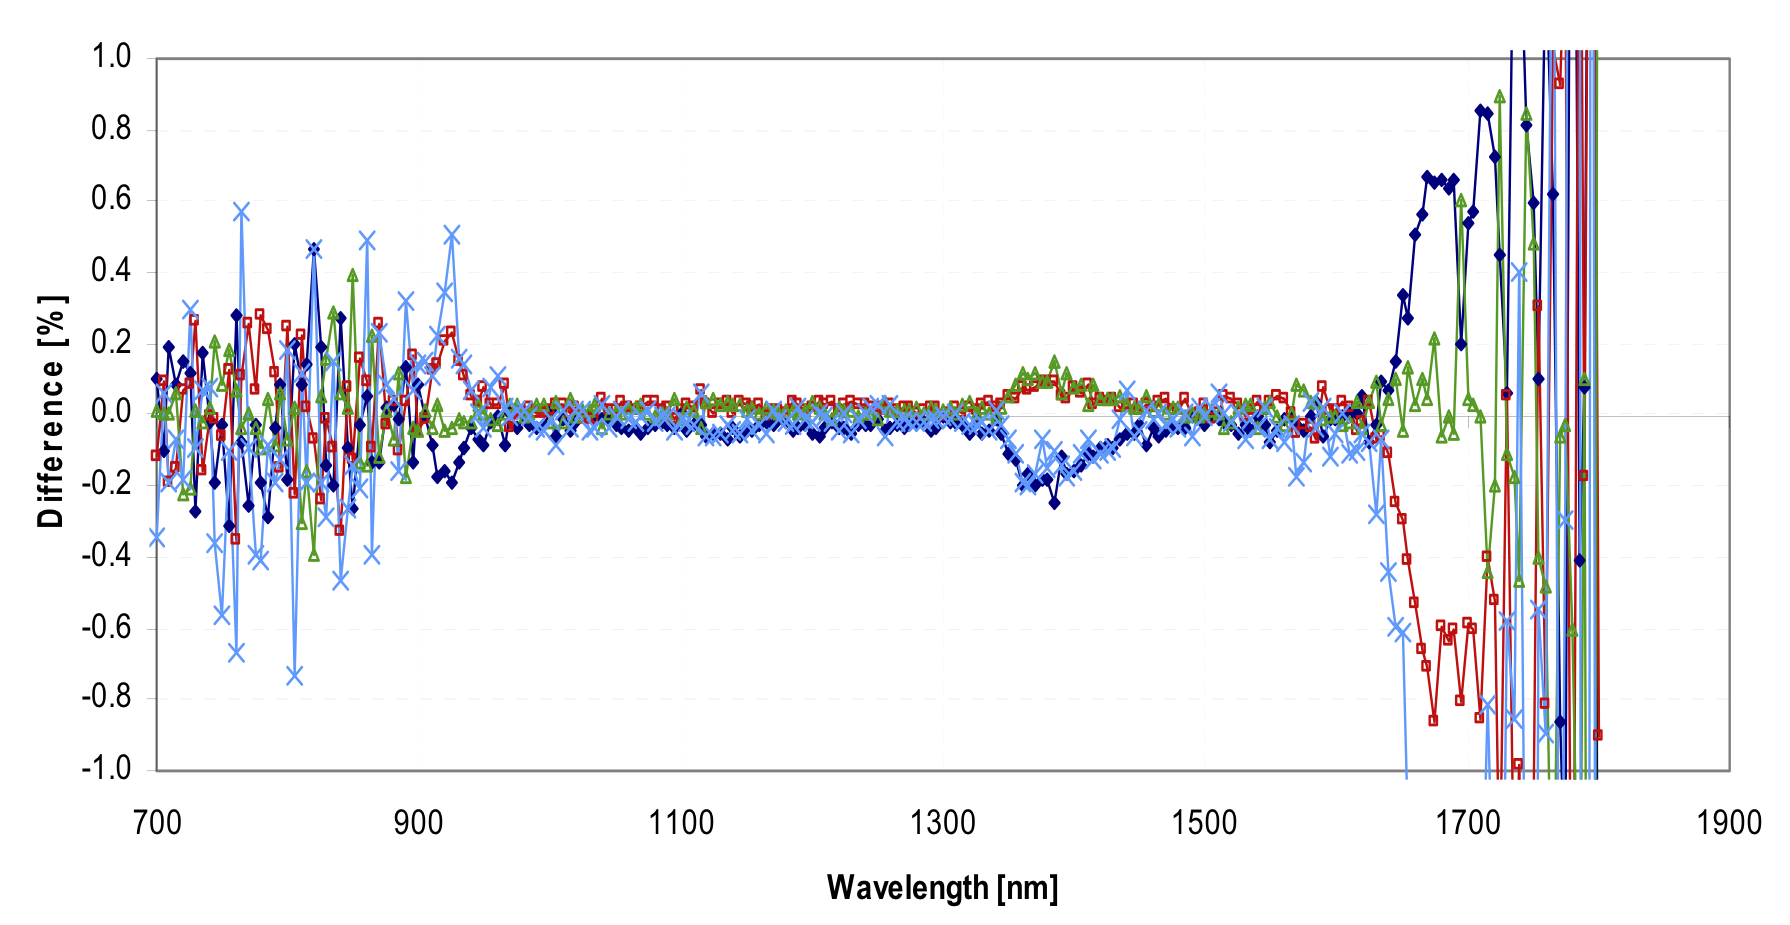
\includegraphics[width=5in]{NIST_diode2}}
\caption{{\small
{\bf Quantum efficiency curve and fractional uncertainty for
NIST-calibrated photodiode, from \citet{Stubbs2010a} and
\citet{Eppeldauer09}.}  Panel \ref{diodeStubbs}: Between 400 and 900~nm, calibration
methods already in use in test systems indicate photodiode accuracy is
better than 0.1\%, as in the bottom part of this panel.  The sudden
decrease in calibration accuracy below 900~nm is due to calibration
methods used by NIST in 2005. Panel \ref{diodeEppel}: More recent photodiode
calibration efforts by \citet{Eppeldauer09} show better than 0.1\%
accuracy can be achieved to beyond 1200~nm, the limit of detector
response for LSST, as shown here in the response curves resulting from
multiple scans of a single source using the same photodiode.} }
\label{fig:NIST_diode}
\end{minipage}
}
\end{figure}


\begin{figure}
\centering
\fbox{
\begin{minipage}{6.5in}
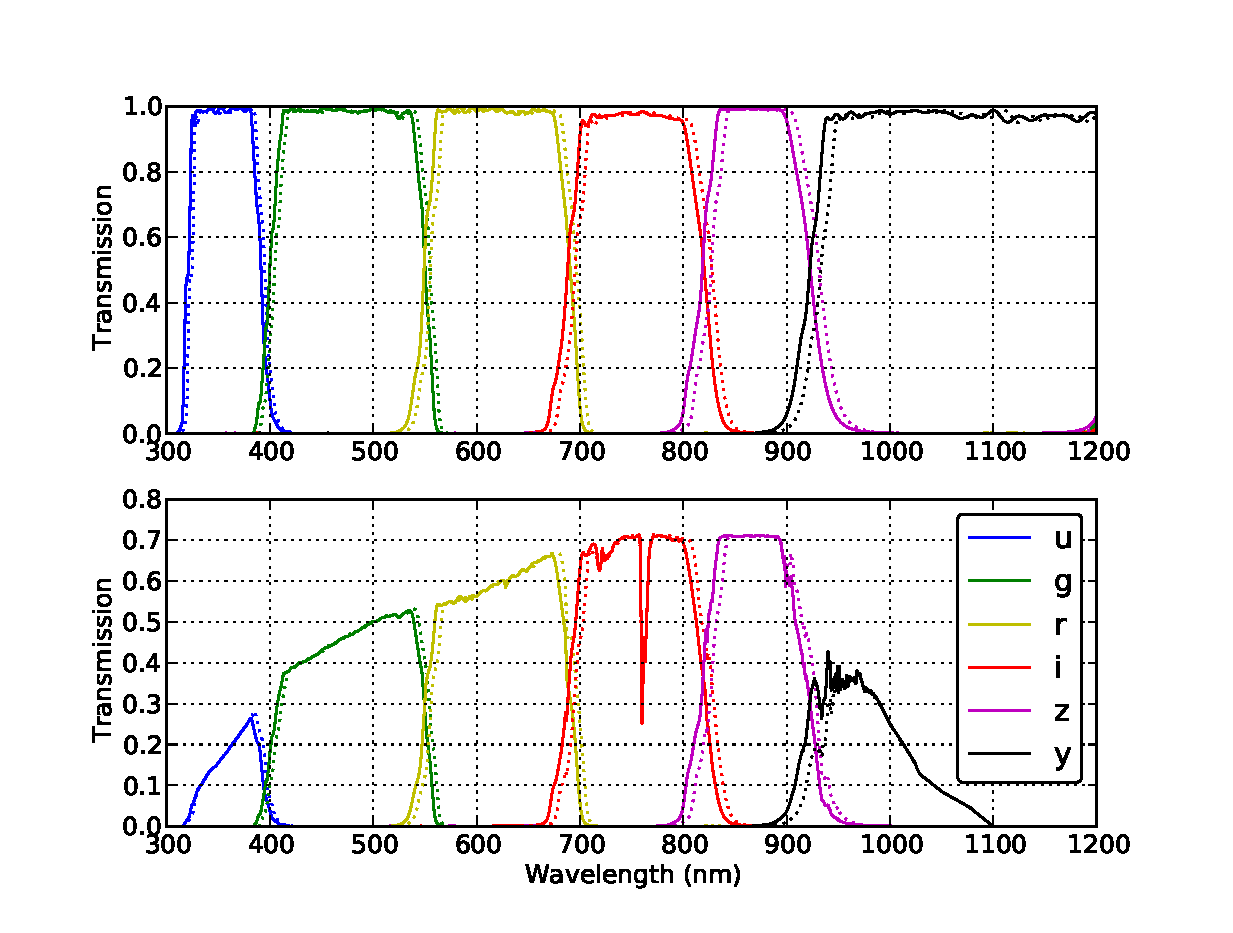
\includegraphics[width=6in]{filter_shifts}
\caption{{\small 
{\bf Baseline filter curves and a potential (1\% of the central
  wavelength) shift due to nonuniformity in the filter bandpass.}
The solid lines indicate standard filter bandpasses (top panel: filter
alone, bottom panel: filter plus standard mirror, lens, detector and atmosphere
response curves) while the dashed lines indicate the same bandpass
shifted redward by 1\% of the central wavelength.}}
\label{fig:filtershift}
\end{minipage}
}
\end{figure}

\clearpage

\begin{figure}
\centering
\fbox{
\begin{minipage}{6.5in}
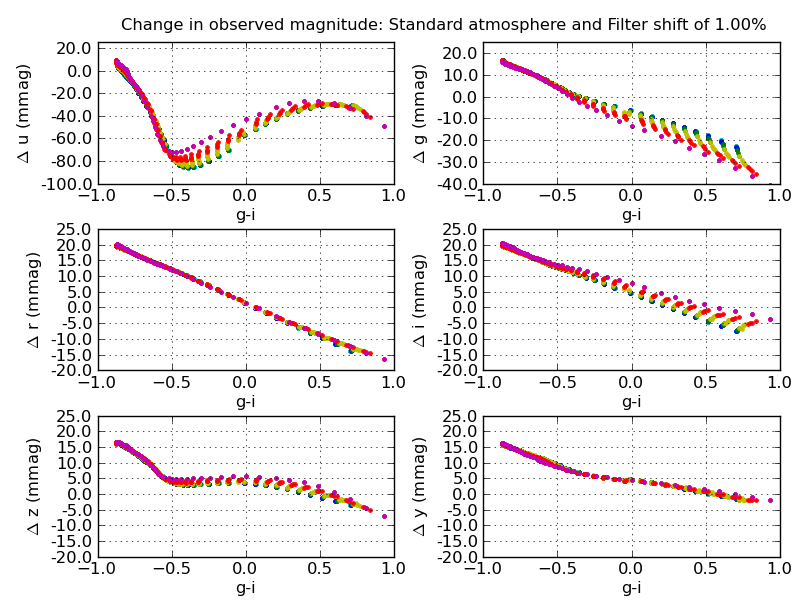
\includegraphics[width=6in]{delta_mags_filtershift}
\caption{{\small 
{\bf $\Delta m_b^{obs}$
due to a hardware response curve shift of 1\% of the central
wavelength of each bandpass.}  850 main sequence star Kurucz models with temperatures
between 5000K and 35000K and metallicity indexes between -5.0 and 1.0
(solar) were combined with a standard atmosphere and standard
hardware bandpass, and then with a total system response where the
atmosphere remained constant but the hardware response was shifted by
1\% of the central wavelength of each bandpass (as in
Fig~\ref{fig:filtershift}). The points in each plot are color-coded by metallicity, in
steps of 1 dex between -5.0 (blue) to 1.0 (magenta). The resulting
changes in observed 
natural magnitudes are on the order of
20~mmag typically, except in $u$ band where the shift can create a
$\delta u$ of closer to 80~mmag for certain temperatures of main sequence
stars. By measuring the bandpass shape as a function of radius and the
colors of the main sequence stars, we can remove these effects.} }
\label{fig:dmag_filtershift}
\end{minipage}
}
\end{figure}

%\begin{figure}
%\centering
%\fbox{
%\begin{minipage}{6.5in}
%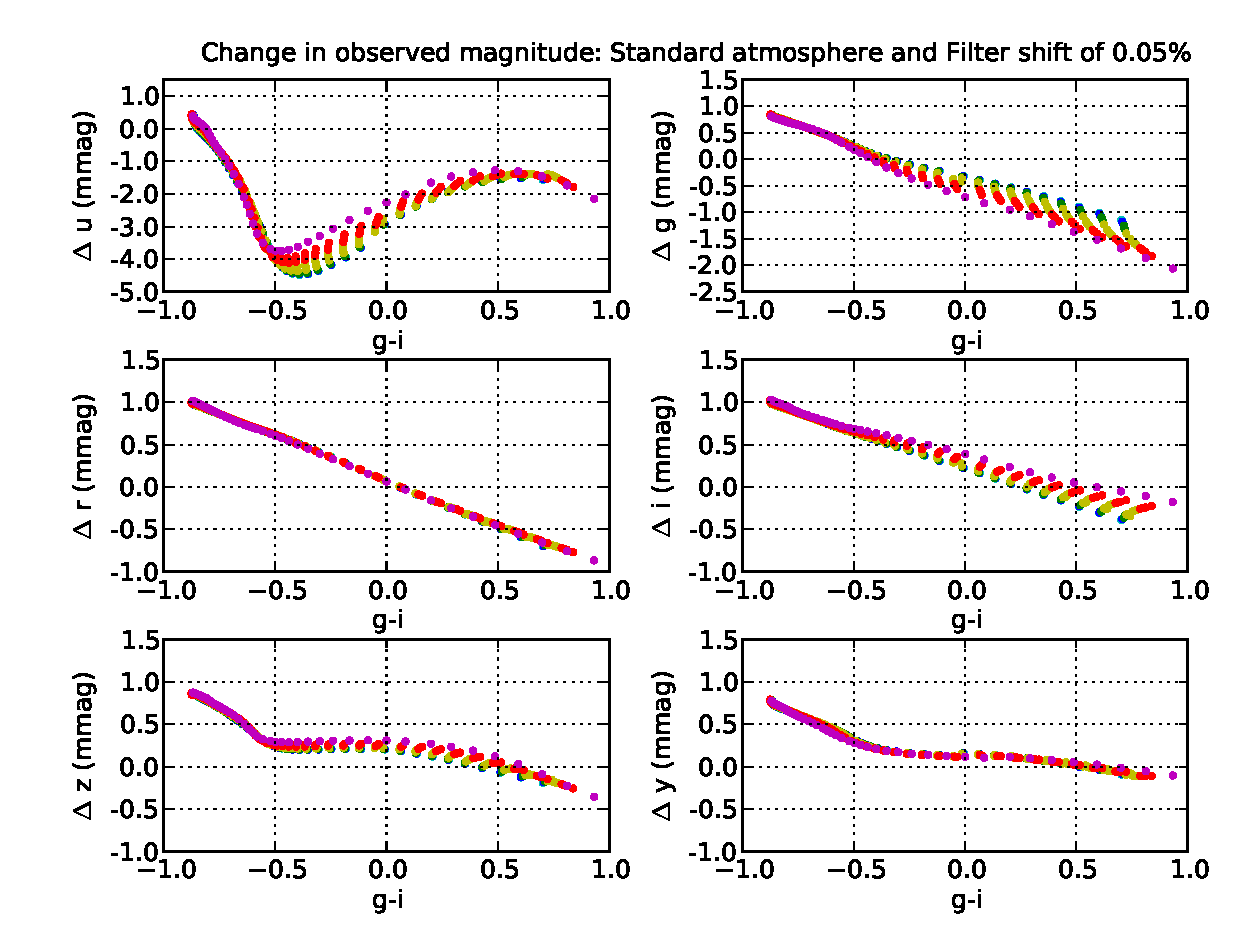
\includegraphics[width=6in]{delta_mags_filtershift_small}
%\caption{{\small 
%{\bf $\Delta m_b^{obs}$ due to a hardware
%response curve shift of 0.05\% of the central wavelength of each
%bandpass.} Similar to Fig~\ref{fig:dmag_filtershift} except that the
%hardware response was shifted by only 0.05\% of the central
%wavelength, an amount representing an unmeasured shift in the hardware
%response and thus contributing directly to the final error in the
%calibration of the natural magnitudes. Note that the $y$ scale in
%these plots is reduced by a factor of 20 from
%Figure~\ref{fig:dmag_filtershift}, consistent with measuring and
%compensating for the
%bandpass shift to within a 0.05\% error. }}
%\label{fig:dmag_filtershift_small} 
%\end{minipage}
%}
%\end{figure}
 



\begin{figure}[htpb]
\centering
\fbox{
\begin{minipage}{6.5in}
\subfloat[\label{lowairmass}]{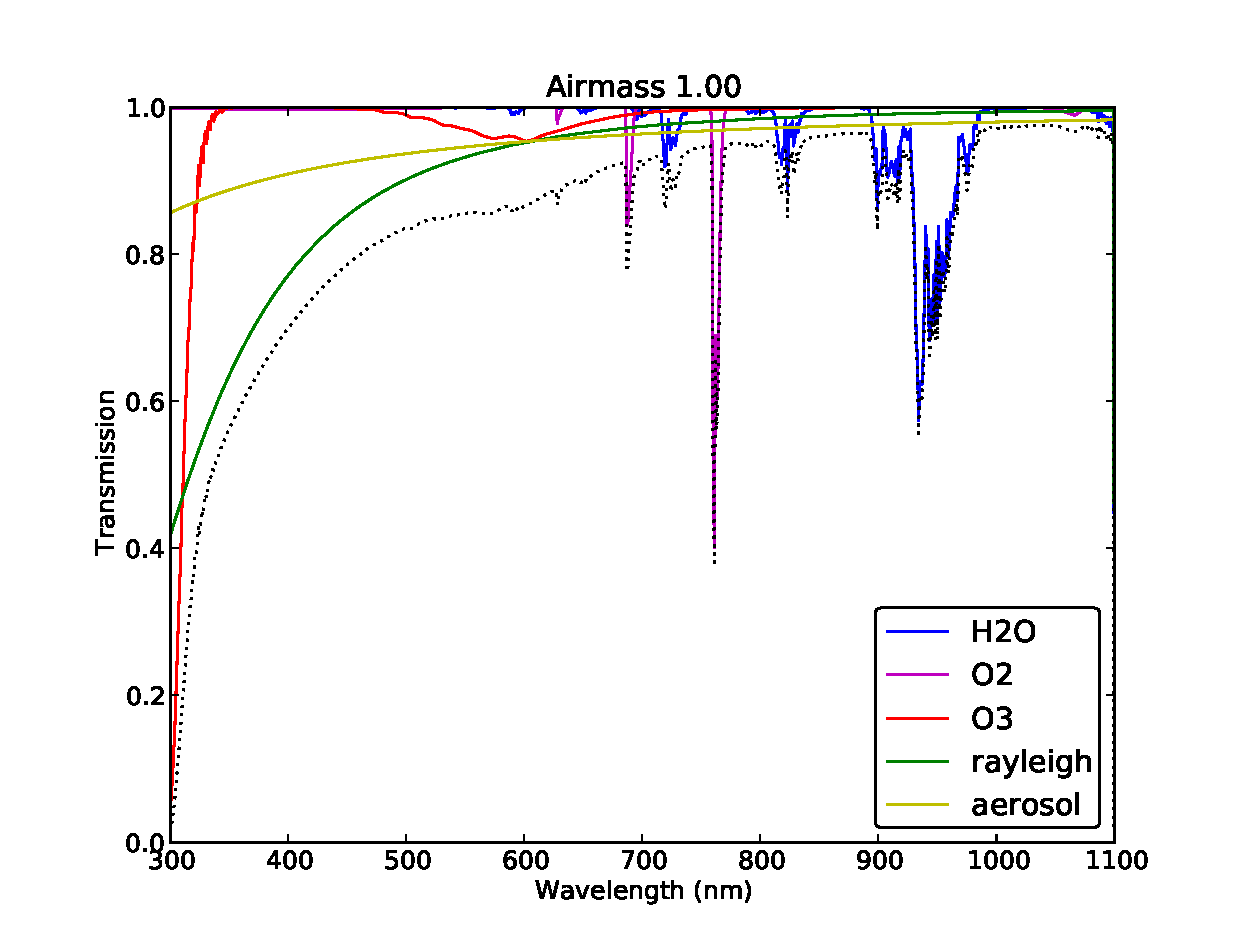
\includegraphics[width=4in]{absorption_compsA}}\\
\vspace{-10pt}
\subfloat[\label{hiairmass}]{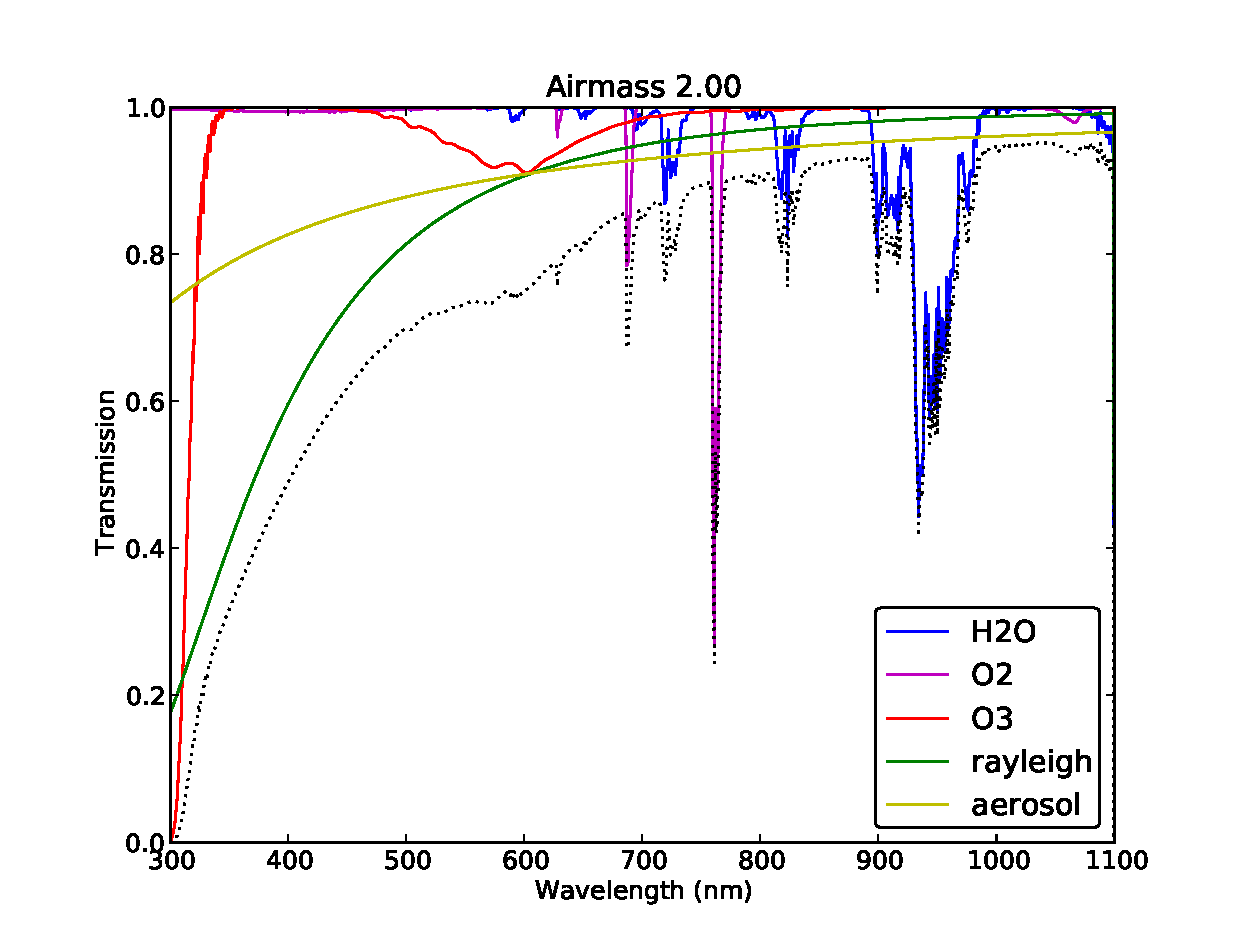
\includegraphics[width=4in]{absorption_compsB}} 
\caption{{\small
{\bf Components of atmospheric absorption.} The wavelength dependence
of  various atmospheric absorption components at zenith
(Panel \ref{lowairmass}) and at airmass=2.0 (Panel \ref{hiairmass}) are shown here.  The \water\,(blue) and
\ozone\,(red) molecular absorption contributions are shown separately,
while the \oxy\,absorption is combined with other trace elements
(magenta). A typical example of aerosol scattering (Mie scattering) is
included (yellow), as is molecular scattering (Rayleigh scattering)
(green). All components except aerosol scattering were generated using
MODTRAN4 with the US Standard option (aerosol scattering is not part
of the US Standard atmosphere). The resulting total absorption curve
is the product of each of these effects and is shown with the dotted
black line. This is an illustrative atmosphere; under actual observing
conditions the molecular absorption components will vary in strength
with time and the square root of the airmass, the molecular and
aerosol scattering will depend on airmass, and the aerosol scattering
profile will also vary with time.}}
\label{fig:absorption_comps}
\end{minipage}
}
\end{figure}


\begin{figure}[htb]
\centering
\fbox{
\begin{minipage}{6.5in}
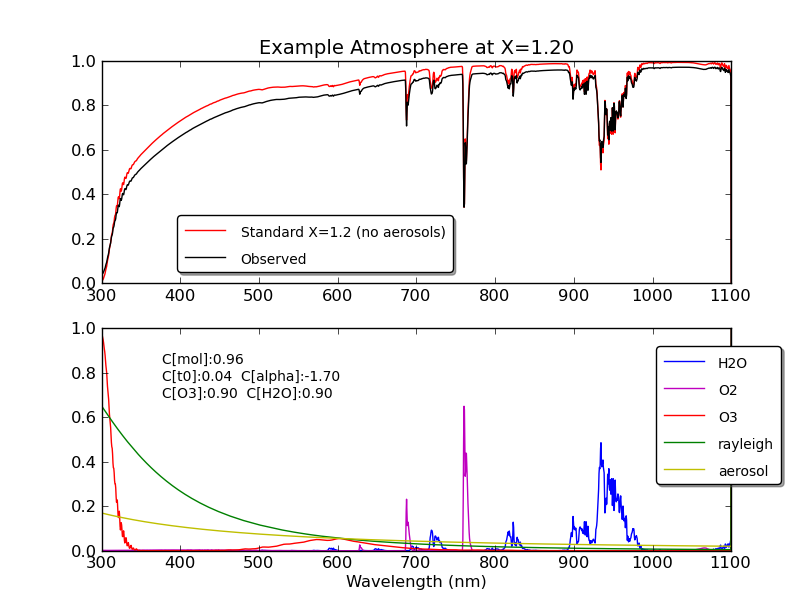
\includegraphics[width=6in]{atmo_airmass12}
\caption{{\small
{\bf Example of an atmosphere generated from a typical mix of
atmospheric components.} The bottom panel shows the MODTRAN absorption
templates at this airmass used in generating the final atmosphere
(the $A_{rayleigh/\oxy/\ozone/\water}$ and $A_{aerosol} = 1-e^{\tau_{aerosol}}$ from
Equation~\ref{eqn:atmo_fit}). The top panel shows the final combined atmospheric
transmission curve in black, as well as a `standardized' atmospheric transmission
curve in red. This demonstrates that (even without using the full
MODTRAN software, just the transmission templates) that we can closely
recreate any atmosphere desired with any composition.} }
\label{fig:absorption_comps2}
\end{minipage}
}
\end{figure}

\clearpage

\begin{figure}
\centering
\centering
\fbox{
\begin{minipage}{6.5in}
\subfloat[]{\label{a}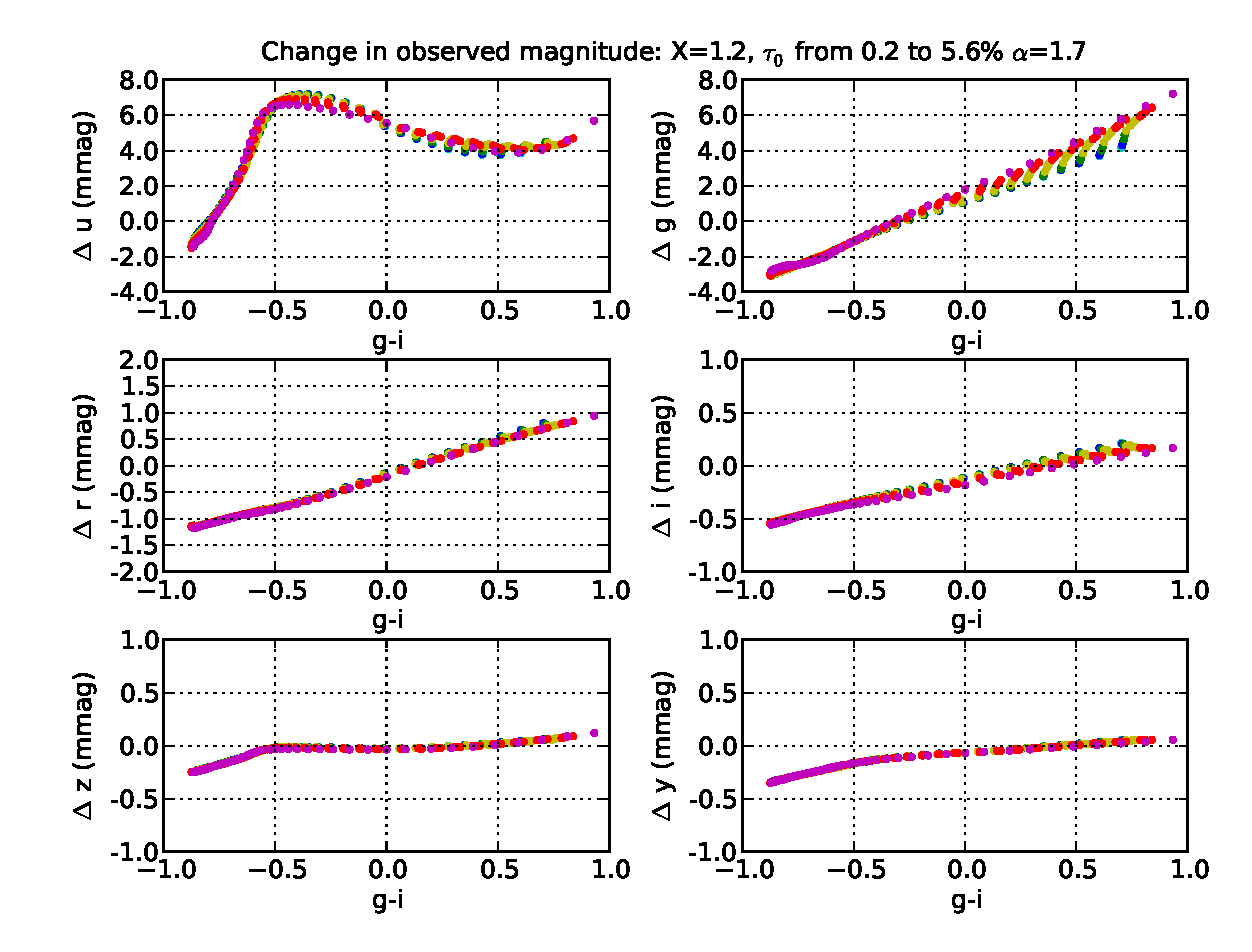
\includegraphics[width=3.2in]{delta_mags_t0full}}
\subfloat[]{\label{b}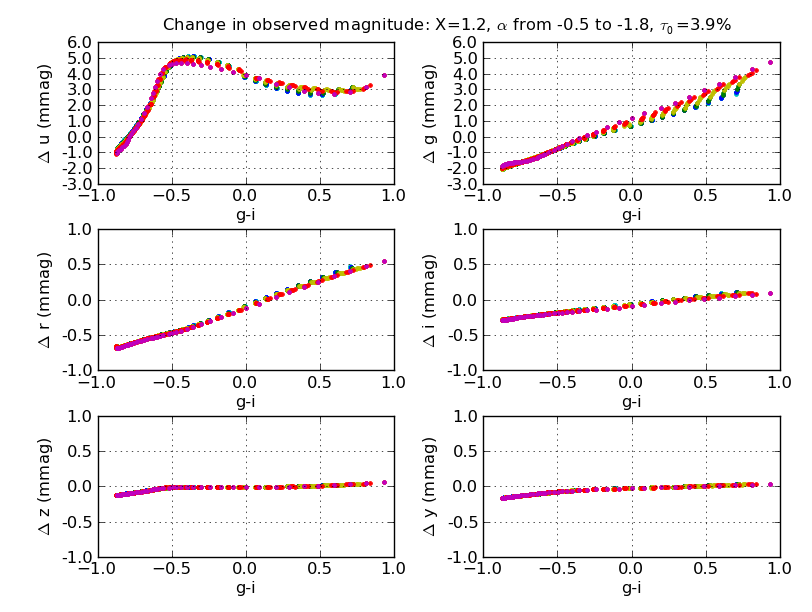
\includegraphics[width=3.2in]{delta_mags_alphafull}} \\
\subfloat[]{\label{c}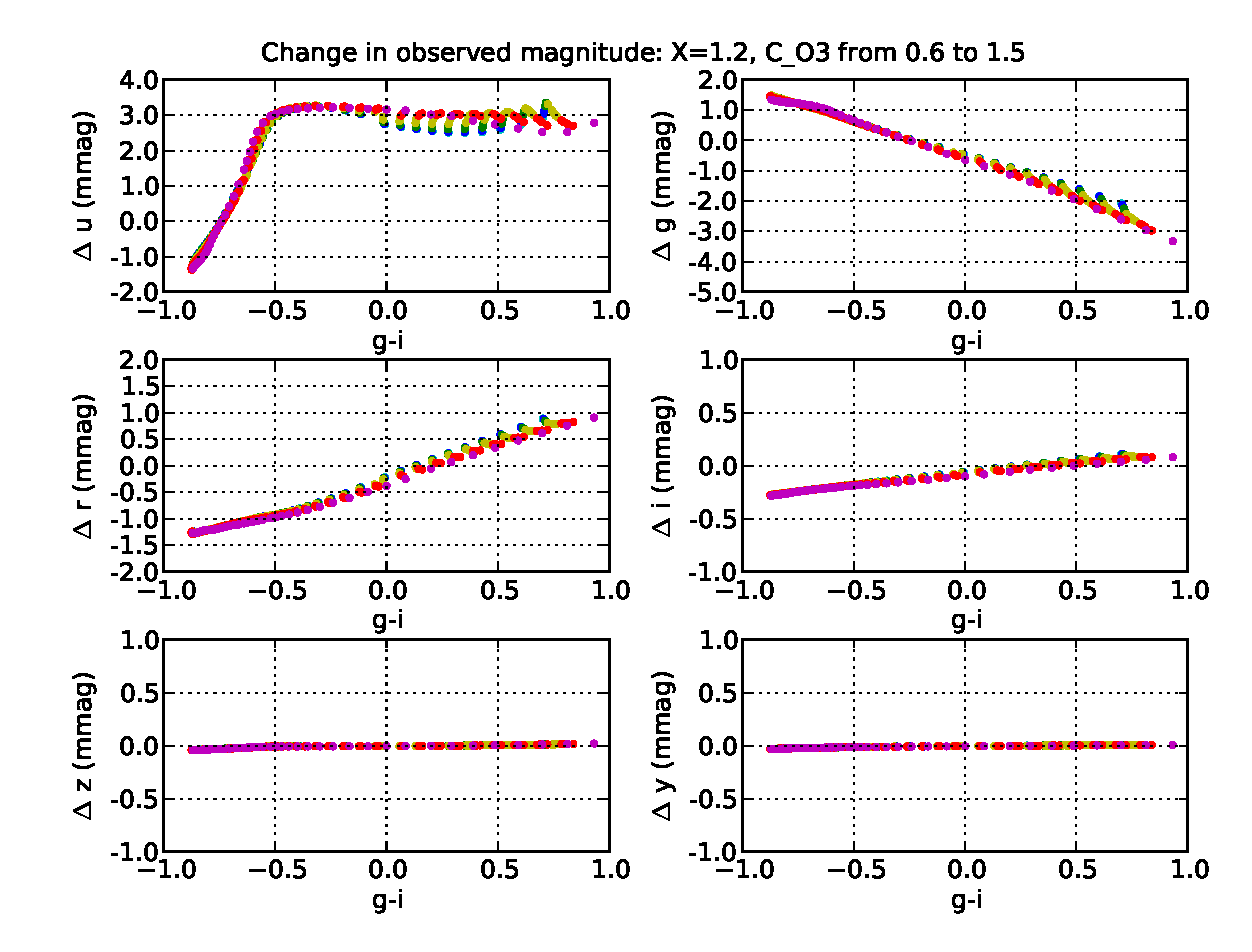
\includegraphics[width=3.2in]{delta_mags_O3full}}
\subfloat[]{\label{d}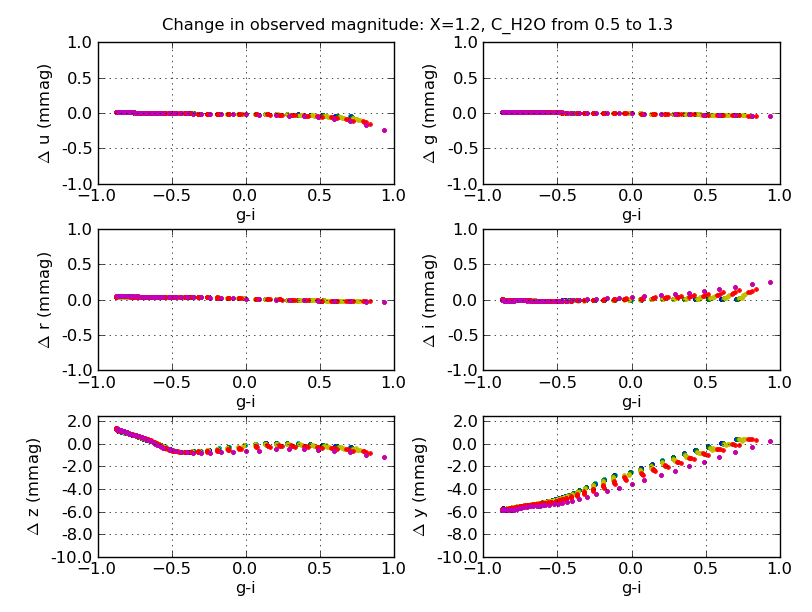
\includegraphics[width=3.2in]{delta_mags_H2Ofull}} 
\caption{{\small
{\bf $\Delta m_b^{obs}$ due to variations of each
individual absorption component.} Each atmospheric transmission curve
(at X=1.2) was combined with the set of main sequence Kurucz curves to
determine the resulting changes in observed magnitudes, as in
Figure~\ref{fig:dmag_filtershift}. Panels \ref{a} and \ref{b} show the
effects of varying aerosol absorption in $\tau_0$ and $\alpha$
respectively, Panel \ref{c} shows the effect of varying \ozone\,absorption. These
effects are concentrated in $u$ and $g$ bands, with a negligible effect
in $izy$. Panel \ref{d} shows the effect of varying the \water\,absorption,
which is strongest in $y$, with some effect in $z$ and no effect in
$ugri$.
}}
\label{fig:dmag_atm_comps}
\end{minipage}
}
\end{figure}

\begin{figure}
\centering
\centering
\fbox{
\begin{minipage}{6.5in}
\subfloat[]{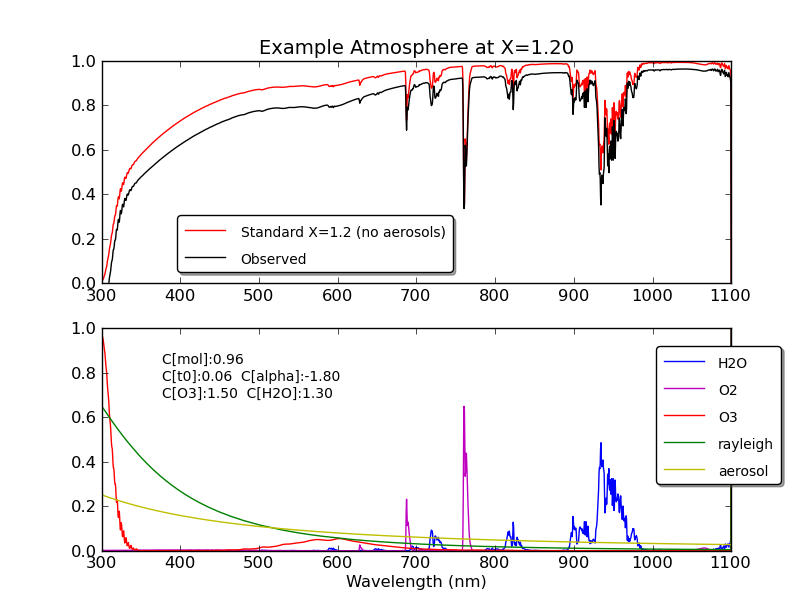
\includegraphics[width=5in]{atmo_max}} \\
\subfloat[]{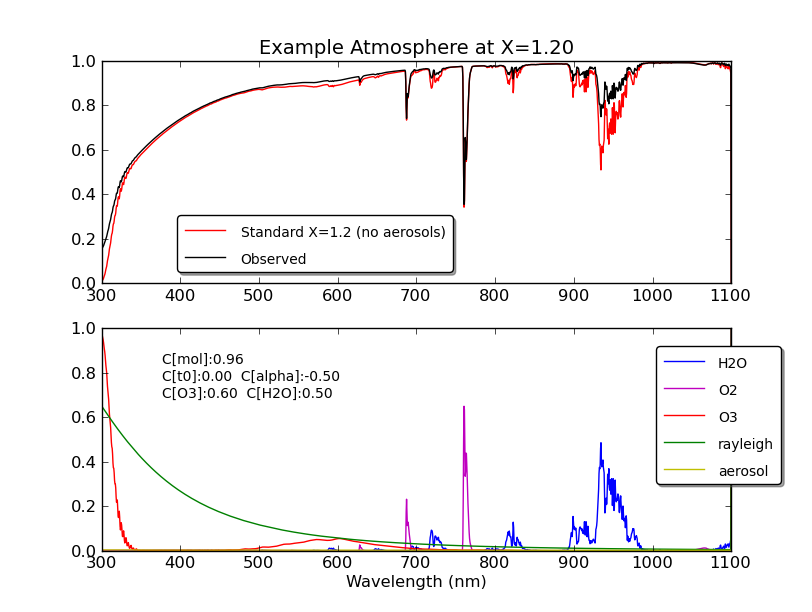
\includegraphics[width=5in]{atmo_min}}
\caption{{\small  {\bf `Extreme' atmospheres generated from MODTRAN profiles and extremes 
of atmospheric coefficients.} Using the extremes of $C_{\water}$, $C_{\ozone}$,
and $\tau_0$ and $\alpha$ from \citet{Burke2010b}, two test atmospheres
with $X=1.2$ were created using Equation~\ref{eqn:atmo_fit}. }}
\label{fig:atm_changes}
\end{minipage}
}
\end{figure}

\begin{figure}
\centering
\centering
\fbox{
\begin{minipage}{6.5in}
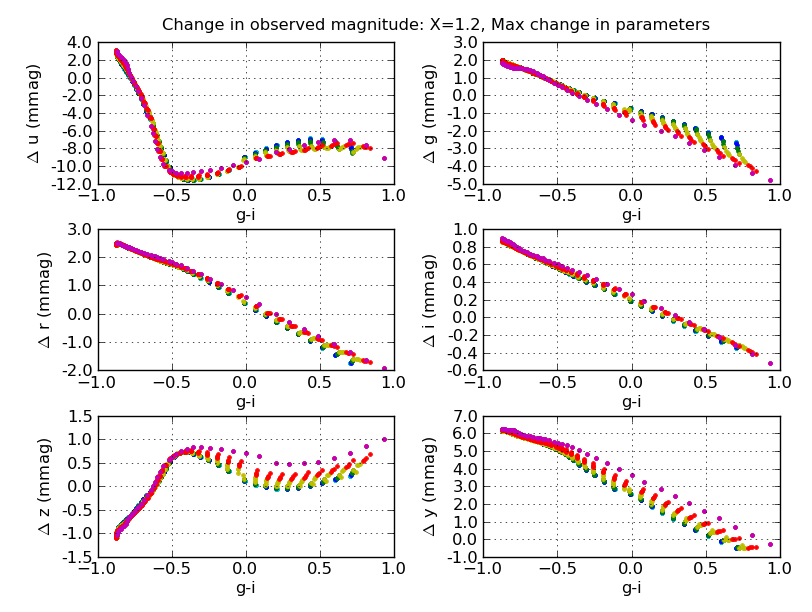
\includegraphics[width=6in]{delta_mags_max}
\caption{{\small
{\bf$\Delta m_b^{obs}$ due to `extreme' variations of 
atmospheric transmission.} Two atmospheric transmission curves were 
created using Equation~\ref{eqn:atmo_fit} and the widest variations of
atmospheric extinction coefficients from \citet{Burke2010b}. The wavelength
profile of these atmospheres is shown in Figure~\ref{fig:atm_changes}. 
These atmospheric transmission curves were combined with the baseline LSST 
hardware transmission curves, and used to generate magnitudes for 850 Kurucz
models with temperatures between 5000~K and 35000~K and metallicities between
-5.0 and 1.0 (solar). The resulting differences in natural magnitudes between 
the two extremes of the atmospheric transmission in each filter are shown above. 
}}
\label{fig:dmag_atm_max}
\end{minipage}
}
\end{figure}

%\begin{figure}
%\centering
%\centering
%\fbox{
%\begin{minipage}{6.5in}
%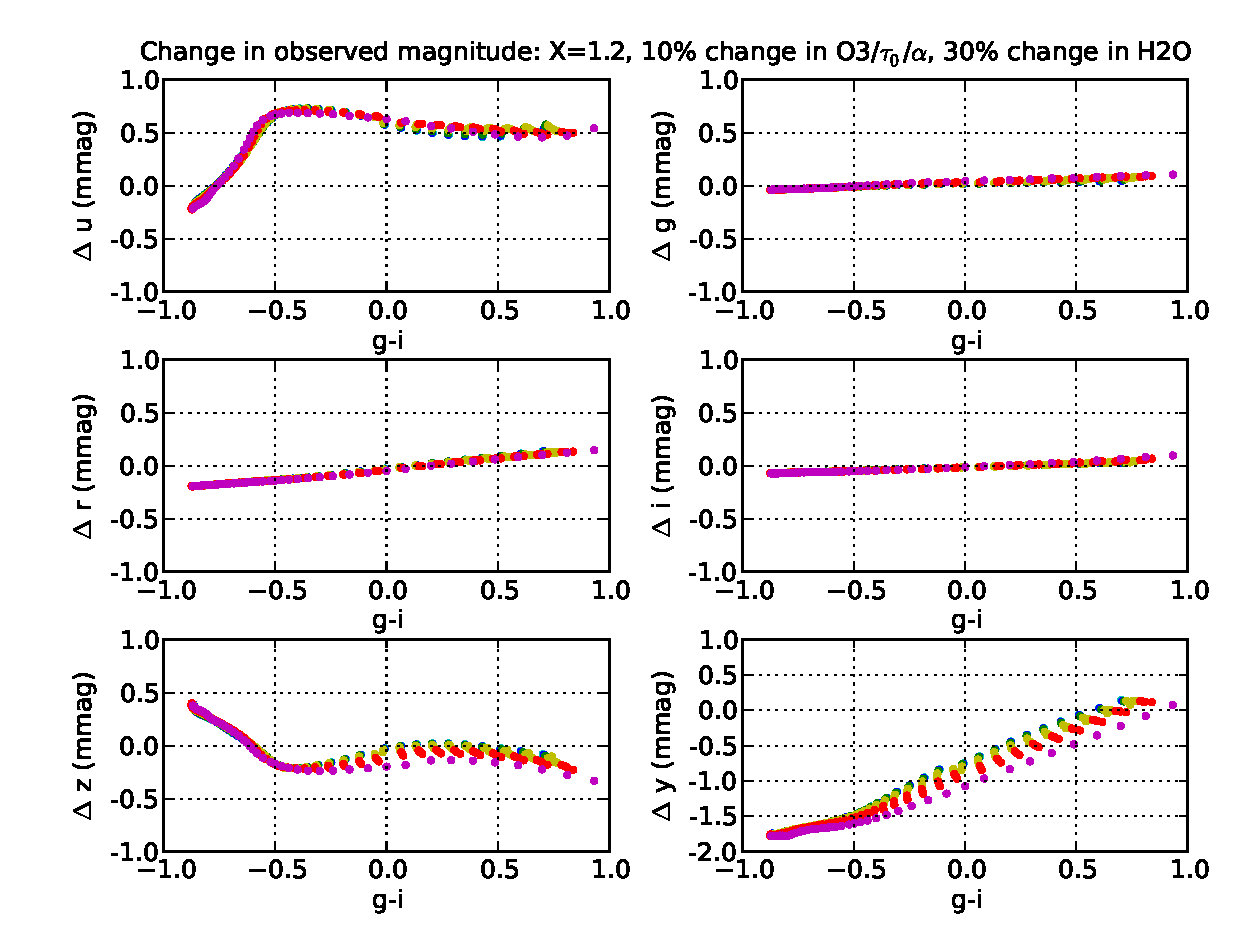
\includegraphics[width=6in]{delta_mags_10}
%\caption{{\small
%{\bf $\Delta m_b^{obs}$ due to 10\% variations of 
%atmospheric transmission in \ozone\,and aerosol, with 30\% variation of \water.} 
%This is similar to Figure~\ref{fig:dmag_atm_max}, except $C_{\ozone}$,
%$\tau_0$ and $\alpha$ were only varied by 10\% of the total range of
%values measured in \citet{Burke2010b}, and $C_{\water}$ was varied by 30\%
%of the total range. }}
%\label{fig:dmag_atm_10}
%\end{minipage}
%}
%\end{figure}


\begin{figure}[htbp]
\centering
\fbox{
\begin{minipage}{6.5in}
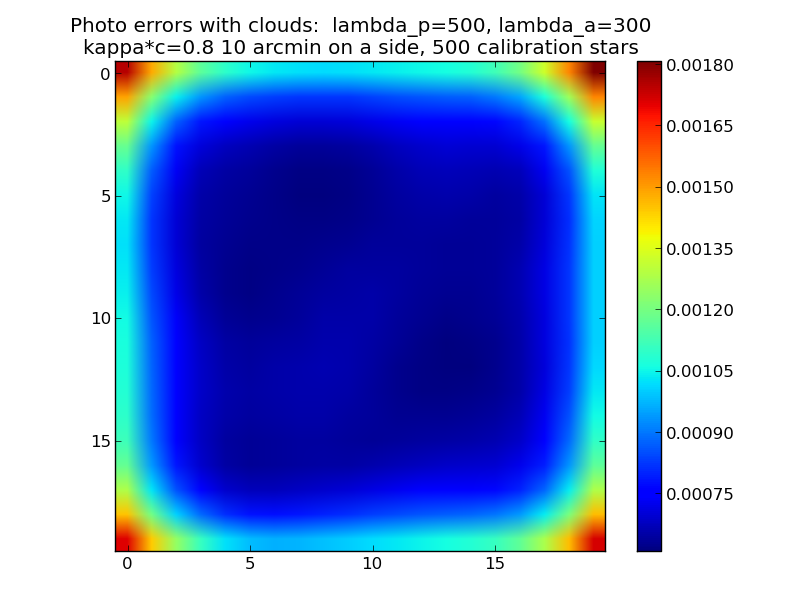
\includegraphics[width=6.5in]{CloudSfFigs/PhotoErrs1.png}
\caption{ {\small {\bf Gauss-Markov predictions for zeropoint errors from clouds with average extinction
of 0.8 mag, characteristic scale 500 meters, and averaging length 300 meters.} }
\label{fig:GaussMarkov} }
\end{minipage}
}
\end{figure}

\clearpage

\begin{figure}[htbp]
\centering
\fbox{
\begin{minipage}{6.5in}
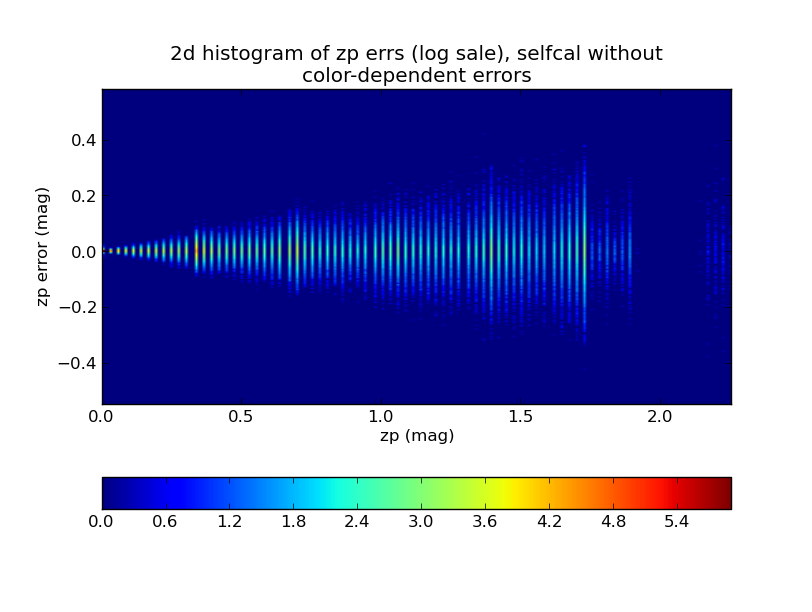
\includegraphics[width=6.5in]{SelfcalFigs/zp_errs_2d.png}
\caption{ {\small {\bf Zeropoint errors vs zeropoint, from a self calibration simulation without color-dependent
errors.  The color scale
shows the log10 of the number of samples at that point.  The periodic behavior of the zeropoint density is an
artifact of OpSim's treatment of cloud cover.} }
\label{fig:zp2dhist} }
\end{minipage}
}
\end{figure}

\begin{figure}[htbp]
\centering
\fbox{
\begin{minipage}{6.5in}
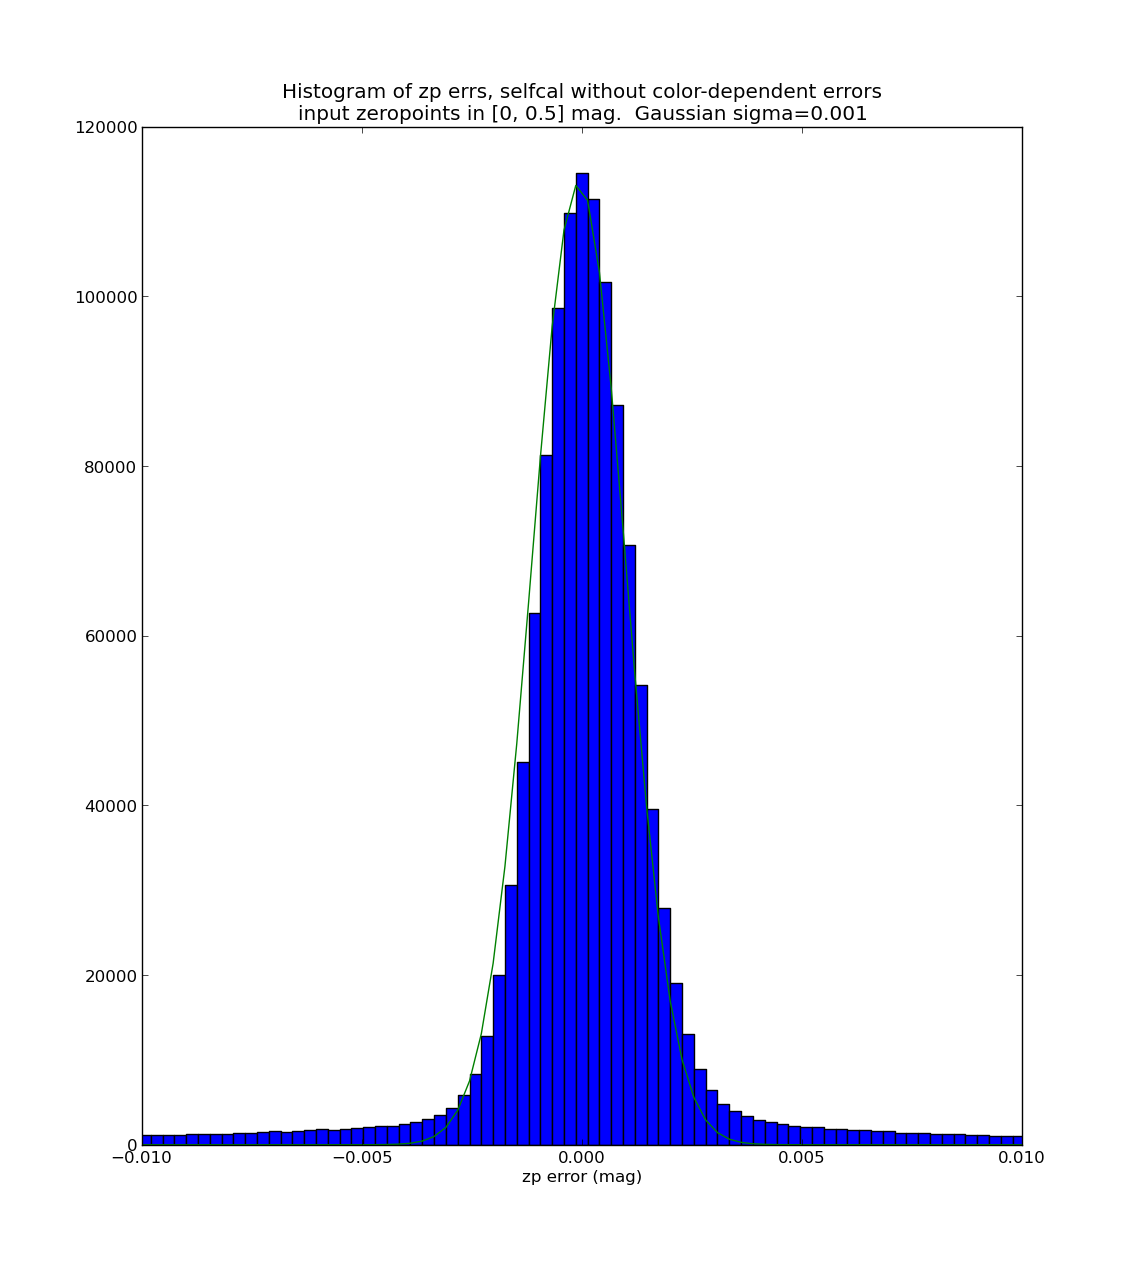
\includegraphics[width=6.5in]{SelfcalFigs/zp_errs_0_05_w_gaussian.png}
\caption{ {\small {\bf Zeropoint errors vs zeropoint, from a self calibration simulation without color-dependent
errors. The histogram shows a vertical crossection of the error fan, with zeropoint in the range $0 < zp < 0.5 mag$} }
\label{fig:zpHist0_0.5} }
\end{minipage}
}
\end{figure}

\begin{figure}[htbp]
\centering
\fbox{
\begin{minipage}{6.5in}
\includegraphics[width=6.5in]{SelfcalFigs/zp_errs_10_15_w_gaussian.png}
\caption{ {\small {\bf Zeropoint errors vs zeropoint, from a self calibration simulation without color-dependent
errors. The histogram shows a vertical crossection of the error fan, with zeropoint in the range $1.0 < zp < 1.5 mag$} }
\label{fig:zpHist1.0_1.5} }
\end{minipage}
}
\end{figure}


\begin{landscape}
\begin{center}
\begin{table}[htb]
\caption{{\bf Repeatability error budget.  All values are in mmag} }
\begin{tabular}{l | l | c c c c c c }
Affected term & Effect &  $u$  & $g$ & $r$ & $i$ & $z$ & $y$ \\ \hline
{\bf $m_b^{obs}$} & {\bf Total} & 3.0 & 3.0 & 3.0 & 3.0 & 3.0 & 3.0 \\ \hline
{\bf $\Delta m_b^{obs}$} & & & & \\
& Atmospheric water vapor errors & 0.2 & 0 & 0 & 0 & 1.0 & 2.0  \\
& Atmospheric aerosol and ozone errors & 1.6 & 2.1 & 0.1 & 0 & 0 & 0  \\
& Undetected atmospheric variability & 1.4 & 0.7 & 0 & 0 & 0 & 0 \\
& Monochromatic illumination correction errors & 3.0 & 0.5 & 0.8 & 0.5 & 0.1 & 0.6\\
& Photodiode monitoring system errors & 0.8 & 0.5 & 0 & 0 & 0 & 0.1 \\
& Calibration star SED errors & 5.6 & 0.8 & 0.5 & 0.4 & 0.4 & 0.2 \\
& Focal plane temperature errors & 0 & 0 & 0 & 0 & 0 & 0.2 \\ 
& {\bf Total} & 6.7 & 2.5 & 0.9 & 0.6 & 1.1 & 2.1 \\ \hline
$Z_b^{obs}$ & & & & \\
& Clouds and cloud-like effects (90\% of obs) & 1.0 & 1.0 & 1.0 & 1.0 & 1.0 & 1.0 \\
& Camera gain variation (short term) & 1.0 & 1.0 & 1.0 & 1.0 & 1.0 & 1.0 \\
& {\bf Total} & 1.4 & 1.4 & 1.4 & 1.4 & 1.4 & 1.4 \\ \hline
{\bf Total} & & 7.5 & 4.1 & 3.5 & 3.4 & 3.5 & 3.9 \\ \hline
{\bf Design Requirement} & & 7.5 & 5.0 & 5.0 & 5.0 & 7.5 & 7.5 \\ 
{\bf Min. Requirement} & & 12 & 8.0 & 8.0 & 8.0 & 12 & 12 \\
\end{tabular}
\label{tab:rpt_error_budget}
\end{table}
\end{center}
\end{landscape}

\begin{figure}[htbp]
\centering
\fbox{
\begin{minipage}{6.5in}
\includegraphics[width=6.5in]{SelfcalFigs/RA_Dec_radius}
\caption{ {\small {\bf Pattern of focal plane radius across sky} }
\label{fig:RA_Dec_radius} }
\end{minipage}
}
\end{figure}

\begin{figure}[htbp]
\centering
\fbox{
\begin{minipage}{6.5in}
\includegraphics[width=6.5in]{SelfcalFigs/RA_Dec_Zp}
\caption{ {\small {\bf Pattern of cloud zeropoints across sky} }
\label{fig:RA_Dec_Zp} }
\end{minipage}
}
\end{figure}

\clearpage

\begin{figure}
\centering
\fbox{
\begin{minipage}{6.5in}
\subfloat[]{\label{a}\includegraphics[width=3.2in]{PDerrorsInp}} 
\subfloat[]{\label{b}\includegraphics[width=3.2in]{PDerrors1}}
\caption{{\small
{\bf $\Delta m_b^{obs}$ due to systematic errors in photodiode response.  Panel \ref{a} shows
the randomly chosen input error curve for the photodiode.  Panel \ref{b} shows the effect
on Kurucz SEDs.}
}}
\label{fig:PDerrs}
\end{minipage}
}
\end{figure}

\begin{figure}[htbp]
\centering
\fbox{
\begin{minipage}{6.5in}
\includegraphics[width=6.5in]{fpTempEffects.png}
\caption{ {\small {\bf Effect of 0.5 deg K variation in focal plane temperature on natural mags} }
\label{fig:TempVarEffects} }
\end{minipage}
}
\end{figure}

\begin{figure}[h!]
\centering
\centering
\fbox{
\begin{minipage}{6.5in}
\includegraphics[width=5in]{filters}
\caption{{\small {\bf The baseline LSST filter set.}}
\label{fig:filterset}}
\end{minipage}
}
\end{figure}



\begin{figure}[htbp]
\centering
\fbox{
\begin{minipage}{6.5in}
\includegraphics[width=6in]{AtmoFigs/SNAerosol_04vs16.png}
\caption{ {Effect on natural mags of SN1a of variation of aerosol optical depth from 0.04 to 0.16 mag} 
\label{fig:SNAerosol} }
\end{minipage}
}
\end{figure}

\begin{figure}
\centering
\centering
\fbox{
\begin{minipage}{6.5in}
\includegraphics[width=6in]{dmag_all_max+shift}
\caption{{\small
{\bf $\Delta m_b^{obs}$ due to changes in a hardware bandpass shift
  and a maximum change in atmospheric absorption components.}  This
plot is similar in nature to a combination of
Figure~\ref{fig:dmag_filtershift} and \ref{fig:dmag_atm_max}, but has
been extended to include a wider variety of object SEDs. Main sequence
stars are shown as the sequence of purple dots, and Mdwarfs are
shown as the sequence of blue 'x's. The large round circles represent
a quasar SED at various redshifts, color-coded with redshift as
follows: $0<z<1$ is blue, $1<z<2$ is green, and $2<z<3$ is red. The
large filled squares show the change in natural magnitudes for SNIa
templates at times of 0, 20, and 40 days from peak; $0<z<0.36$ are
blue squares, $0.36<z<0.72$ are green squares, and $0.72<z<1$ SNIa are
red squares. 
}}
\label{fig:dmag_allseds}
\end{minipage}
}
\end{figure}

\begin{figure}
\centering
\centering
\fbox{
\begin{minipage}{6.5in}
\includegraphics[width=6in]{HardwareFigs/CalypsoSite}
\caption{{\small
The auxiliary telescope is sited adjacent to LSST
}}
\label{fig:CalypsoSite}
\end{minipage}
}

\end{figure}
\begin{figure}
\centering
\centering
\fbox{
\begin{minipage}{6.5in}
\includegraphics[width=6in]{HardwareFigs/calypso}
\caption{{\small
The auxiliary telescope 
}}
\label{fig:auxtel}
\end{minipage}
}
\end{figure}

\end{figure}
\begin{figure}
\centering
\centering
\fbox{
\begin{minipage}{6.5in}
\includegraphics[width=6in]{HardwareFigs/DomeScreenOLD}
\caption{{\small
The flat field illumination system
}}
\label{fig:domescreen}
\end{minipage}
}
\end{figure}

\begin{figure}
\centering
\centering
\fbox{
\begin{minipage}{6.5in}
\subfloat[\label{nobs}]{\includegraphics[width=3.2in]{SelfcalFigs/r_1e6/Snobs}}
\subfloat[\label{sdmag}]{\includegraphics[width=3.2in]{SelfcalFigs/r_1e6/Sdmag}} \\
\subfloat[\label{starstrue}]{\includegraphics[width=3.2in]{SelfcalFigs/r_1e6/Sdamg_hist}}
\subfloat[\label{starsrms}]{\includegraphics[width=3.2in]{SelfcalFigs/r_1e6/Srepeat_IQR_bright_hist}} 
\caption{{\small {\bf Results from a self-calibration simulation.}
Panel \ref{nobs} shows the number of visits across the sky for the
first two years of the survey in $r$-band.  The color range has been
truncated since the deep-drilling fields can have over 1000 visits.
Conditions for this simulation are described in the text.  Panel
\ref{sdmag} shows the true minus best-fit stellar magnitudes residuals
across the sky after iterating the self-calibration solver. Panel
\ref{starstrue} shows similar information, but as a histogram of all
stars, demonstrating the `uniformity' requirement in the SRD. Panel
\ref{starsrms} shows a histogram of the RMS of the difference between
the calibrated and true magnitudes for bright stars, demonstrating the
`repeatability' requirement in the SRD.  }}
\label{fig:selfcal_fiducial}
\end{minipage}
}
\end{figure}

\begin{figure}
\centering
\fbox{
\begin{minipage}{6.5in}
\plottwo{SelfcalFigs/HPid_8.png}{SelfcalFigs/HPid_16.png}
\caption{HEALpixel maps for 8 and 16 sides, resulting in 400 and 1568 individual pixels in the Southern hemisphere respectively.}
\end{minipage}
}
\end{figure}


\begin{figure}
\centering
\fbox{
\begin{minipage}{6.5in}
\plottwo{SelfcalFigs/r_1e6_regsolver/Sdmag.png}{SelfcalFigs/r_1e6/Sdmag.png}
\plottwo{SelfcalFigs/r_1e6_regsolver/Sdamg_hist.png}{SelfcalFigs/r_1e6/Sdamg_hist.png}
%\plottwo{SelfcalFigs/r_1e6_regsolver/Srepeat_IQR.png}{SelfcalFigs/r_1e6/Srepeat_IQR.png}
%\plottwo{SelfcalFigs/r_1e6_regsolver/Srepeat_IQR_bright_hist.png}{SelfcalFigs/r_1e6/Srepeat_IQR_bright_hist.png}
\caption{Comparison of a simulation solved simultaneously (left) with one solved on individual HEALpixels and combined.  Statistically, the differences between the two solutions are at the sub-millimag level, which is much less than the differences we see between runs with different starting seeds (Figure~\ref{fig:diffseed}). \label{fig:hpvglobal}}
\end{minipage}
}
\end{figure}

\begin{figure}
\centering
\centering
\fbox{
\begin{minipage}{6.5in}
\includegraphics[width=6in]{AuxtelesFigs/stdERvResSNR210withSpectro.png}
\caption{{\small
Errors in atmospheric transmission functions determined over 7 nights with 80 spectra per night.  The x axis is the spectrograph
resolution.  Improvement of resolution beyond 400 does not improve the accuracy.  This may be linked to the similar resolution of
the Kurucz spectra used for the stars. 
}}
\label{fig:SpectroRes}
\end{minipage}
}
\end{figure}

\begin{figure}
\centering
\centering
\fbox{
\begin{minipage}{6.5in}
\includegraphics[width=6in]{DataReleaseProduction}
\caption{{\small
Data Release Production
}}
\label{fig:auxtel}
\end{minipage}
}
\end{figure}
\end{document}